%% Source : gabarit de thèse de l'Université Laval (memoire.tex)
%%
%% Modifié par :
%% Karine Guinard (INRS-ETE, 2014)
%% karine.guinard@ete.inrs.ca
% \PassOptionsToPackage{french,english}{babel}
\documentclass[phd, noindex, hyperref, entetes, prelimtmm, francais, english]{theseINRS} % Pour une
% thèse de doctorat, remplacer "msc" par "phd"
\usepackage[utf8]{inputenc} % Pour pouvoir taper les accent directement et sans
% passer par \'
% \usepackage[bitstream-charter]{mathdesign}
\usepackage{libertine}
\usepackage[libertine,cmintegrals,cmbraces,vvarbb]{newtxmath}
\usepackage[T1]{fontenc} % Pour que les accents soient correctement traités dans
% le PDF

% \usepackage{lmodern} % Pour que les accents soient correctement traités dans
% le PDF
% \usepackage{amsmath,amssymb,bm} % Pour offrir plus de symboles mathématiques
\usepackage{natbib}
% \usepackage[francais,english]{babel}
\bibliographystyle{bibliostyleINRS} % Pour citer des références avec \cite et
% \citep
\usepackage[letterpaper, margin=25mm]{geometry} % Pour la définition de la mise
% en forme du document
\usepackage{graphicx} % Pour insérer des images avec la commande
% \includegraphics
\usepackage{rotating}
\usepackage{pdflscape} % Pour inclure des éléments en mode paysage en conservant
% les entêtes en mode portrait (environnement sideways)
\usepackage{afterpage}

\usepackage{tabularx} % Pour rendre plus flexible la création de tableaux
\usepackage{nomencl} % Pour générer une liste d'abréviations
\usepackage[font={singlespacing,footnotesize,bf}]{caption} % Pour définir le
% style des légendes de figures
\usepackage[font={singlespacing,footnotesize}]{subcaption} % Pour générer des
% sous-figures (subfig is deprecated)
\usepackage{textcomp} % Pour que les symboles de degrés apparaissent plus beaux
\usepackage{emptypage} % Pour enlever les numéros de page sur les pages blanches
\usepackage{calc}
\usepackage[shortlabels]{enumitem}
% \usepackage{enumitem}

\usepackage{epstopdf}
\usepackage{booktabs,dcolumn,caption}
\usepackage{threeparttable}
\usepackage{lineno}
\usepackage{multirow}
\usepackage{hhline}
\usepackage[table]{xcolor}
\usepackage{textcomp}
\usepackage{lineno,hyperref}
\usepackage{microtype}
\usepackage{afterpage}
\usepackage[separate-uncertainty]{siunitx}
\usepackage[version=3]{mhchem}
\usepackage{etoolbox}
% \usepackage[]{chapterbib}
\usepackage[globalcitecopy]{bibunits}
\usepackage{setspace}
\usepackage{lipsum}
\usepackage{blindtext}
\usepackage[noabbrev,french]{cleveref}
\usepackage{bibentry}
\usepackage[]{caption}
\usepackage{subcaption}
\usepackage{textcomp}
\usepackage{tocloft}
\usepackage{translations}
\usepackage{afterpage}
\usepackage{fancyhdr}

\robustify\tnote

\crefname{chapter}{article}{articles}

\global\def\fonteauteurs{}


\captionsetup[subfigure]{labelfont=bf,textfont=bf,singlelinecheck=off,justification=centering}




\sisetup{
list-final-separator = { \translate{and} },
range-phrase = { \translate{to (numerical range)} },
}
\makeatletter
\newcommand\mynobreakpar{\par\nobreak\@afterheading}
\makeatother

\makeatletter
\newcommand{\nolisttopbreak}{\vspace{\topsep}\nobreak\@afterheading}
\makeatother

\usepackage{afterpage}

\newcommand\blankpage{%
    \null
    \thispagestyle{empty}%
    \addtocounter{page}{-1}%
    \newpage}
\definecolor{Gray}{gray}{0.9}
\urlstyle{same}

\DisableLigatures{encoding = *, family = * }
\modulolinenumbers[5]

\sisetup{separate-uncertainty,per-mode = symbol,detect-weight=true,
detect-family=true}

\raggedbottom % Pour uniformiser l'espacement vertical entre les éléments dans
% les pages

%%%%%%%%%%%%%%%%%%%%%%%%%%%%%%%%%%%%%%%%%%%%%%%%%%%%%%%%%%
 % \includeonly{introduction/intro}
 % \includeonly{article1/article1}
 % \includeonly{avPropos/avPropos}
 % \includeonly{methodologie/methodologie}
 % \includeonly{methodologie/sismique_diff}

\begin{document}
    \nobibliography{biblio/biblio}
    \nocite{Perozzi1,Perozzi2}
% \defaultbibliography{biblio/biblio}
% \defaultbibliographystyle{plainnat}
\shorthandoff{:} % Ne pas ajouter automatiquement un espace avant un ":"
\shorthandoff{;} % Ne pas ajouter automatiquement un espace avant un ";"
\shorthandoff{?} % Ne pas ajouter automatiquement un espace avant un "?"
\shorthandoff{!} % Ne pas ajouter automatiquement un espace avant un "!"

\pagesprelim
\PrenomNom{Lorenzo Perozzi}
\titre{ÉLABORATION D'UN FLUX DE TRAVAIL POUR LA SURVEILLANCE SISMIQUE DE
L'INJECTION DU \texorpdfstring{\ce{CO2}}{CO2} DANS DES GRÈS PEU POREUX: DE LA
MODÉLISATION SISMIQUE À L'INVERSION STOCHASTIQUE.} % en lettres majuscules
%\soustitre{Sous-titre} % Si désiré, ajouter un sous-titre
\programme{sciences de la terre}
\grade{\textit{Philosophiae doctor}, Ph.D.}
\jury{Examinateur externe &  Hubert Fabriol Ph.D.\\
	& Bureau de Recherches Géologiques et Minières (BRGM) \\[0.5cm]
	Examinateur externe &  Martin Bèche Ph.D.\\
	& Petrolia \\[0.5cm]
	Examinateur interne & Mathieu Duchesne Ph.D.\\
	& Commission Géologique du Canada (CGC) \\[0.5cm]
	Directeur de recherche & Bernard Giroux Ph.D.\\
	& INRS - Centre Eau Terre Environnement \\[0.5cm]
	Codirecteur de recherche & Erwan Gloaguen Ph.D\\
	& INRS - Centre Eau Terre Environnement \\[0.5cm]
	Codirecteur de recherche & Klaus Holliger Ph.D.\\
	& Université de Lausanne \\[0.5cm]}
\annee{2015}

\maketitle
\afterpage{\blankpage}
\thispagestyle{empty}
\null\vspace{\stretch{1}}
\begin{flushright}
\emph{All models are wrong, but some are useful.}\\
\textsc{- George Box}
\end {flushright}
\vspace{\stretch{2}}\null % Section facultative
\afterpage{\blankpage}
\chapter*{Remerciements}
\addcontentsline{toc}{chapter}{Remerciements} % Ajouter à la table des matières.
\setlength{\parindent}{0cm}
\setlength{\parskip}{1em}
Avec ces remerciements, je voudrais montrer ma reconnaissance aux personnes qui
m'ont aidé à réaliser ce travail, qui m'ont côtoyé et supporté et avec
lesquelles j'ai partagé de très beaux moments pendants ces années à l'INRS. \par

Je tiens tout d’abord à remercier mon directeur de thèse Bernard Giroux. Tu as
su me guider tout au long de ma thèse grâce à des explications toujours
exhaustives, à des conseils et des questions toujours judicieuses.

J’ai eu le privilège d’avoir un codirecteur de thèse très pédagogue et dévoué.
Merci Erwan pour ta disponibilité, ton respect, ta patience, ta compréhension et
ton encouragement durant toutes ces années d’étude. Un jour, j'arriverai aussi à
te battre au tennis.\par
Je remercie Klaus Holliger, mon autre codirecteur de recherche pour son appui à
distance. C'est grâce à toi que mon aventure à Québec a commencé il y a
désormais sept ans.\par

Je tiens à remercier Douglas Schmitt de l’université de l'Alberta qui m’a
accueilli dans son laboratoire de physique des roches. Merci aussi à Randy
Kofman pour son aide précieuse avec les mesures de laboratoire.\par

Je tiens à remercier les membres du jury d’évaluation d’avoir pris le temps de
lire
ma thèse.\par

Pendant mes études, j’ai bénéficié du soutien des collègues de bureaux et de
membres du LIAMG en général, avec lesquels j'ai eu le plaisir de discuter de
science, programmation, mais aussi de la vie de tous les jours. Merci à
Camille, Martin, Jean-Sébastien, Marc, Patrick, Gabriel, Pierre, Mathieu,
Issam.\par

Je tiens à remercier mes parents qui, tout au long de mon parcours, m’ont
soutenu, écouté et encouragé. Merci pour tout ce que vous faites pour moi.\par

Enfin, mais dans mon coeur tu es toujours à la première place, je te remercie
Isabelle. Ton support, ta patience et ton amour inconditionnel m’ont permis
d’atteindre mes objectifs et terminer cette thèse. Merci Éloïse pour toute la
joie que tu nous apportes chaque jour.
 % Section facultative (Remerciements ou
% Avant propos, pas les deux)

\begin{bibunit}[bibliostyleINRS]
\chapter*{Avant-Propos}
% \section{Avant-Propos}
\addcontentsline{toc}{chapter}{Avant-Propos} % Ajouter à la table des matières.
Cette thèse est composée de deux sections distinctes. La première section
comprend une synthèse de l’ensemble des travaux effectués lors du doctorat,
tandis que la deuxième section contient les articles scientifiques qui ont été
écrits suite à ces travaux. Les articles sont:

\begin{enumerate}

	\item \bibentry{Perozzi1}
	\item \bibentry{Perozzi2}

\end{enumerate}
\vspace{5mm}
\noindent
La contribution des auteurs des articles aux projets de recherche s’établit
comme suit:\\

\begin{description}[leftmargin=!,labelwidth=\widthof{\bfseries Randolf S.
Kofman}]
  \setlength\itemsep{1.2em}
  \item[Lorenzo Perozzi] Conception et réalisation des algorithmes, analyse des
données, traitement des données, interprétation des résultats et rédaction des
articles.
  \item[Bernard Giroux]  Conception des projets, contribution à la création des
algorithmes, à l’interprétation des résultats et à la rédaction finale des
articles.
  \item[Erwan Gloaguen]  Conception des projets, contribution à la création des
algorithmes, à l’interprétation des résultats et à la rédaction finale de
l'article 2.
  \item[Douglas R. Schmitt]  Contribution à
l'interprétation des résultats et à la rédaction finale de l’article 1.
  \item[Randolf S. Kofman]  Contribution à la création de données et à la
rédaction finale de l’article 1.
\end{description}
 % Section facultative (Remerciements ou Avant
% propos, pas les deux)
% \bibentry{Perozzi1}
% \putbib[biblio/biblio]
\end{bibunit}
\chapter*{Résumé}
\addcontentsline{toc}{chapter}{Résumé} % Ajouter à la table des matières.
\setlength{\parindent}{0cm}
\setlength{\parskip}{1em}
Plusieurs rapports d'organismes internationaux tels que l'Agence internationale
de l'énergie (AIE) et le Groupe intergouvernemental d'experts sur l’évolution du
climat (GIEC) ont confirmé que le réchauffement climatique est indiscutable et
trouve son origine dans l'activité humaine. En même temps, d'ici \num{2040},
l'AIE prévoit une augmentation de la demande énergétique mondiale de
\SI{37}{\percent}. Bien que le choix des politiques et les évolutions du marché
devraient entraîner une baisse de la demande pour les combustibles fossiles,
ceci ne suffira pas à enrayer l'augmentation des émissions de dioxyde de
carbone, ce qui provoquera une accélération de la hausse de la température
mondiale
de \SI{3.6}{\degreeCelsius} à long terme. Le GIEC estime donc que pour limiter
cette hausse à \SI{2}{\degreeCelsius}, objectif adopté au niveau international
pour prévenir les répercussions les plus graves du changement climatique, le
monde ne devra pas émettre plus de \SI{1000}{\giga\tonne} \ce{CO2} à compter de
\num{2014}. \\
Selon les deux organismes, environ \SI{14}{\percent} des émissions seront
réduites grâce à l'emploi de la technologie du captage et stockage du \ce{CO2}.
Bien que cette technologie ne soit pas universellement reconnue parmi les
agences
de protection de l’environnement et les ONG, elle est la seule méthode à court
terme
qui permettrait d'avoir un impact significatif sur le bilan carbone et il y a
maintenant une urgence pour le déploiement du CSC au-delà de la phase
démonstrative.
Pour que le stockage géologique du \ce{CO2} ait un impact positif sur
l'environnement, le \ce{CO2} doit être stocké dans le sous-sol aussi longtemps
qu'il le faut pour que les émissions anthropologiques chutent à des niveaux
acceptables et dans des roches réservoirs permettant d'accueillir des volumes
importants de \ce{CO2}. Ces contraintes nécessitent que le \ce{CO2} soit stocké
sur
une
échelle de temps de l'ordre de \numrange{e1}{e4} ans. Pour atteindre cette
exigence, on doit s'assurer que le \ce{CO2} reste en place et ne puisse migrer
sur de grandes distances ni verticalement ni horizontalement. \par

À partir de ces constats, cette thèse propose une méthodologie de travail pour
la surveillance sismique temporelle et l’évaluation de l'incertitude liée à
l'injection du \ce{CO2} adaptée à un environnement avec des faibles porosités et
perméabilités, comme celui des Basses-Terres du St-Laurent (BTSL) au Québec,
Canada. Cette
méthodologie est menée sur deux fronts: utiliser les mesures de laboratoire et
la modélisation sismique de puits comme outils de haute résolution pour évaluer la
réponse sismique due à l'injection du \ce{CO2} et définir une séquence logique
de
modélisation stochastique d'un réservoir potentiel pour la séquestration
géologique du \ce{CO2}. Premièrement, les mesures de laboratoire sur deux
échantillons provenant des unités réservoir de BTSL ont permis d'évaluer la
réponse sismique due à l'injection du \ce{CO2} sous différentes conditions de
pression et température. Ces mesures ont permis de calibrer le modèle géologique
utilisé ensuite dans la modélisation sismique de puits. Cette modélisation a
montré que les différences rencontrées aux différents temps sont quantifiables
principalement par un délai de \SI{30}{\milli\second} associé à une diminution
des vitesses quand le \ce{CO2} supercritique remplace la saumure dans l’espace
poreux.\\
Ensuite, la modélisation numérique basée sur un modèle hétérogène réaliste de
l’aquifère salin des BSTL indique qu' à partir des données statiques initiales,
l'approche d'inversion stochastique par déformation graduelle permet
d'obtenir des estimations fidèles des propriétés physiques ainsi qu’une prédiction fiable
de la distribution du \ce{CO2} dans le réservoir.

\chapter*{Abstract}
\addcontentsline{toc}{chapter}{Abstract} % Ajouter à la table des matières.
\setlength{\parindent}{0cm}
\setlength{\parskip}{1em}
Several organizations such as the International Energy Agency (IEA) and the
Intergovernmental Panel on Climate Change (IPCC) confirmed that global warming
is undeniable and originates from human activity.
Following the 4DS IEA scenario, global energy demand is set to grow by
\SI{37}{\percent} by \num{2040}.
While policy choices and market developments bring the share of fossil fuels in
primary energy demand down to just under three-quarters
by 2040, they are not enough to stem the rise in energy-related \ce{CO2}
emissions, which grow by one-fifth. This puts the world on a path consistent
with a long-term global average temperature increase of
\SI{3.6}{\degreeCelsius}.
The IPCC estimates that in order to limit this temperature increase to
\SI{2}{\degreeCelsius} – the internationally agreed goal to avert the most
severe and widespread implications of climate change – the world cannot emit
more than around \num{1000} gigatonnes of \ce{CO2} from \num{2014} onwards.
According to IEA and IPCC, carbon capture and storage (CCS) technology could
reduce \ce{CO2} emissions by \SI{20}{\percent} of \ce{CO2}.
This decade is critical for moving CCS through and beyond the demonstration
phase. This means that urgent action is required, beginning now, from industry
and governments to develop technology and the required business models, and to
implement
incentive
frameworks that can help drive CCS deployment in the power sector and industrial
applications.
If CCS is to have a positive environmental impact then the injected \ce{CO2}
must be stored in geological reservoirs allowing to accommodate huge volumes of
\ce{CO2} for as long as it takes for anthropogenic output rates to drop to
acceptable levels and for the carbon cycle to have recovered and stabilized in
geological reservoirs. This constraint requires \ce{CO2} to be stored for
timescales of the order of \num{e4} or even \num{e4} years. To meet this
requirement we must ensure that it is not possible for injected \ce{CO2} to
migrate on large distances either vertically or horizontally away from the targeted
reservoir. \par

On the basis of these observations, this thesis proposes a workflow for the
timelapse seismic monitoring and the uncertainty assessment of the
\ce{CO2} injection suited to the environment in which porosities and
permeabilities are very low such as the St. Lawrence Lowlands (Québec, Canada) context.
This two-pronged approach use first laboratory measurements and vertical
seismic profiling as high resolution tool in order to assess the seismic
response generated by \ce{CO2} injections. Then, a logical sequence of
stochastic modeling of a potential reservoir for \ce{CO2} sequestration is
defined.
Laboratory measurements on two geological samples from the reservoir units
of the St Lawrence Lowlands has allowed to assess the seismic
response under various temperature and pressions conditions. The results
obtained have helped to calibrate the geological model employed in the seismic
modeling step. The results of the seismic modeling showed that the seismic
signature of the \ce{CO2} is mainly observable by a delay of
\SI{30}{\milli\second} related to a decrease in the wave velocities when
supercritical \ce{CO2} replace brine in the pore space.\\
Numerical experiments based on a realistic heterogeneous saline aquifer model
indicates that, given initial static data, the inversion approach should allow
for faithful properties estimation and reliable prediction of the spatial
distribution of \ce{CO2}.


\cleardoublepage
\phantomsection
\addcontentsline{toc}{chapter}{\contentsname} % Ajouter une ligne pour la table
% des matières dans la table des matières.
\begin{bibunit}[bibliostyleINRS]

\tableofcontents

\cleardoublepage
\phantomsection
\renewcommand*\listfigurename{Liste des figures} % Afficher "Liste des figures"
% plutôt que "Table des figures".
\addcontentsline{toc}{chapter}{\listfigurename} % Ajouter une ligne pour la
% table des figures dans la table des matières.
\listoffigures % Omettre s'il n'y a pas de figure.
\cftaddtitleline{lof}{chapter}{Première partie - Synthèse}{}
\cftaddtitleline{lot}{chapter}{Première partie - Synthèse}{}

\cleardoublepage
\phantomsection
\addcontentsline{toc}{chapter}{\listtablename} % Ajouter une ligne pour la liste
% des tableaux dans la table des matières.
\listoftables % Omettre s'il n'y a pas de tableau.

\cleardoublepage
\phantomsection
% \renewcommand{\nomname}{Liste des abréviations}
% \addcontentsline{toc}{chapter}{\nomname} % Ajouter une ligne pour la liste des
% abréviations dans la table des matières.
% \makenomenclature
% \setlength\nomlabelwidth{2cm} % Aligner les descriptions d'abréviations à 2
% cm.
% \printnomenclature
% \cleardoublepage
% \putbib[biblio/biblio]
\end{bibunit}
\corps
\renewcommand{\tablename}{\textsc{Tableau}} % Afficher "Tableau" plutôt que
% "Table" dans le document.

\part{Synthèse} % Omettre si thèse/mémoire traditionnel, conserver uniquement
% les chapitres

\begin{bibunit}[bibliostyleINRS]

%!TeX root = Thesis_LP.tex
\chapter{Introduction}
\setlength{\parindent}{0cm}
\setlength{\parskip}{1em}
Selon le dernier rapport du Groupe d'experts intergouvernemental sur l’évolution
du climat (GIEC), le réchauffement climatique est indiscutable et
trouve son origine dans l'activité humaine \citep{IPCC2014}. L’atmosphère et les
océans se sont
réchauffés, les quantités de neige et de glace ont diminué et les niveaux des
océans ont augmenté. \\
À partir de l'ère préindustrielle, les émissions des gaz à effet de serre (GES)
ont augmenté principalement à cause de l'industrialisation et de l'augmentation
de la population. Ceci a mené à l'accélération sans précédent de l'augmentation
des
concentrations atmosphériques de dioxyde de carbone de méthane et de protoxyde
d'azote (voir \Cref{fig:GES}).
Il faut s'attendre à ce que la poursuite des émissions de GES aggrave encore la
hausse des températures et provoque de nouveaux changements.
\section{Le problème du charbon}
La concentration du \ce{CO2} dans l’atmosphère varie de façon naturelle. La
\cref{fig:CO2} montre la variation des concentrations de \ce{CO2} dans les
derniers \num{650000} ans \citep{Epica,Siple,Vostok,WMO14}. Ces données montrent
une
concentration stable de
\ce{CO2} d'environ \SI{280}{ppm}, qui correspond à la concentration à la fin de
la dernière glaciation (\num{\pm 10000}). L'augmentation du \ce{CO2} au-dessus
de \SI{280}{ppm}
coïncide avec la révolution industrielle (autour des années 1800) et elle a
accéléré sans cesse jusqu'à nos jours pour atteindre la valeur d'environ
\SI{400}{ppm} en \num{2014}.
\begin{figure}[ht]
        \centering
        \begin{subfigure}[b]{.77\textwidth}
                \caption{Concentrations atmosphériques du \ce{CO2}, \ce{N2O} et
du \ce{CH4}.}
                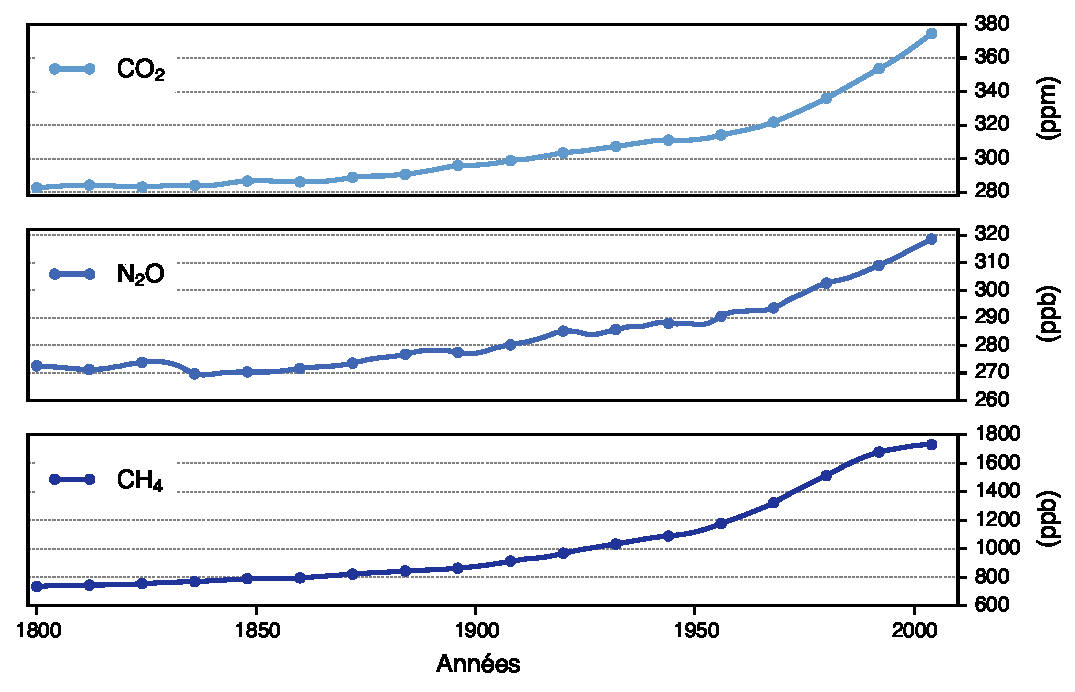
\includegraphics[width=\textwidth]{fig/GES.pdf}
                \label{fig:GES}
        \end{subfigure}%

        \begin{subfigure}[b]{.77\textwidth}
        		\caption{Concentration de \ce{CO2} dans l'atmosphère dans les
dernières \num{650000} années.}
                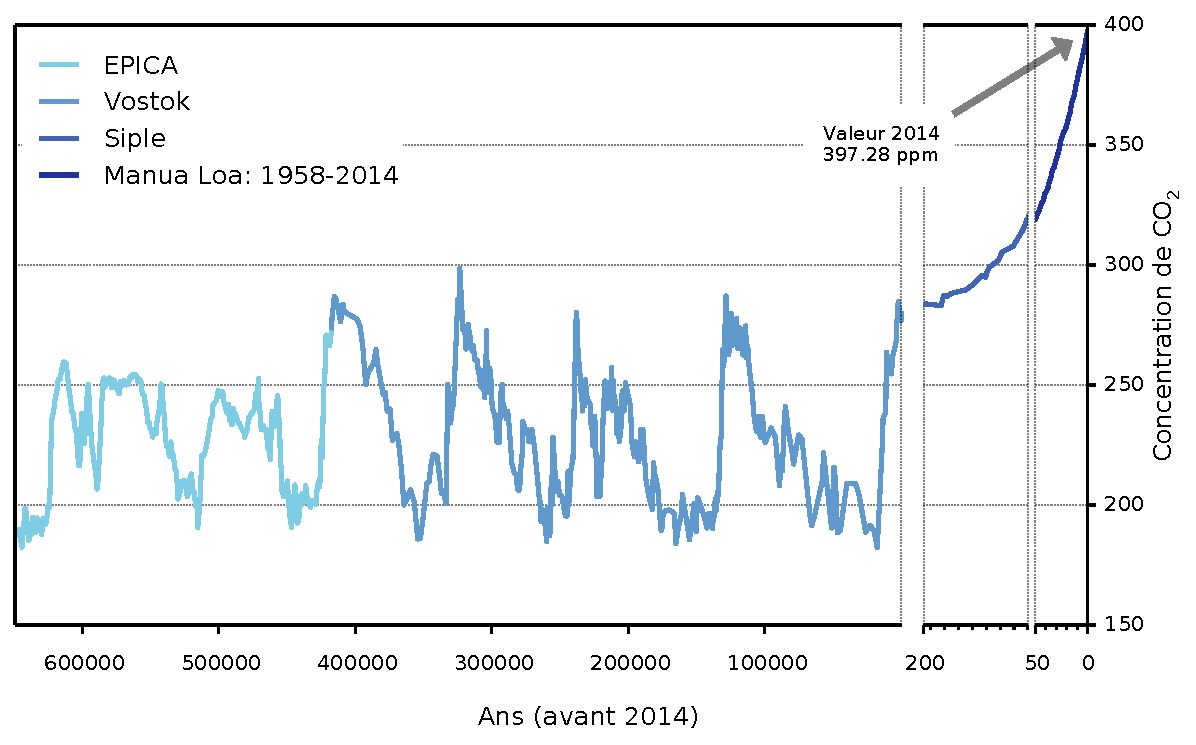
\includegraphics[width=\textwidth]{fig/CO2.pdf}
                \label{fig:CO2}
        \end{subfigure}

        \caption{Évolution des concentrations des gaz à effet de serre dans
l'atmosphère. Source des données: \citet{Epica,Siple,Vostok,WMO14} et
\url{http://www.esrl.noaa.gov/gmd/ccgg/trends}}\label{fig:GES_tot}.
\end{figure}
À partir de ces données, on peut conclure que les concentrations actuelles de
\ce{CO2} dépassent d’au moins 100 ppm le seuil d'équilibre naturel associé au
stade interglaciaire actuel. On peut aussi conclure que la concentration de
\ce{CO2} enregistrée en \num{2014} dépasse d'environ \SI{30}{\percent} les
concentrations plus élevées dans les \num{650000} dernières années. \\
Le méthane \ce{CH4} est le deuxième plus important des gaz à effet de serre. Environ
\SI{40}{\percent} des rejets de \ce{CH4} dans l'atmosphère sont d'origine
naturelle (zones humides) et \SI{60}{\percent} d'origine humaine (élevage de
bétail, riziculture, exploitation des combustibles fossiles, décharges,
combustion de biomasse) \citep{WMO2014}. Le \ce{CH4} atmosphérique a atteint un
nouveau pic en \num{2013} – \num{1824} parties par milliard (ppb) environ – en
raison de l'accroissement des émissions anthropiques. Après une période de
stabilisation, la teneur de l'atmosphère en méthane augmente de nouveau depuis
\num{2007} \citep{WMO2014}.\\
Parmi les activités humaines qui produisent des gaz à effet de serre, la
production d’énergie est de loin la plus grande source de GES et en particulier
de \ce{CO2}. La contribution de l'agriculture (qui produit principalement du
\ce{CH4} et du \ce{N2O}) et des processus industriels non reliés à la production
d'énergie est largement plus faible, comme c'est montré dans la
\cref{fig:CO2_Fossil} \citep{IEA_fossil}.
Dans l'industrie de l'énergie, le \ce{CO2} produit lors de l'utilisation des
combustibles fossiles, domine les émissions totales des GES. Personne ne peut plus nier
que la demande croissante d'énergie à partir de combustibles fossiles a un rôle
clé dans la tendance à la hausse des émissions de \ce{CO2}. Depuis la révolution
industrielle, le \ce{CO2} émis annuellement à partir des combustibles fossiles
a augmenté dramatiquement de presque \num{0} à environ \SI{32}{\giga\tonne}
\ce{CO2} en \num{2012} \citep{IEA_fossil}.\\
Dans un contexte où la demande d’énergie est de plus en plus grande, il faut
trouver des mesures permettant la mise en œuvre d'options durables en matière
de production, de distribution et de consommation finale d'énergie.
\begin{figure}[ht]
\centering
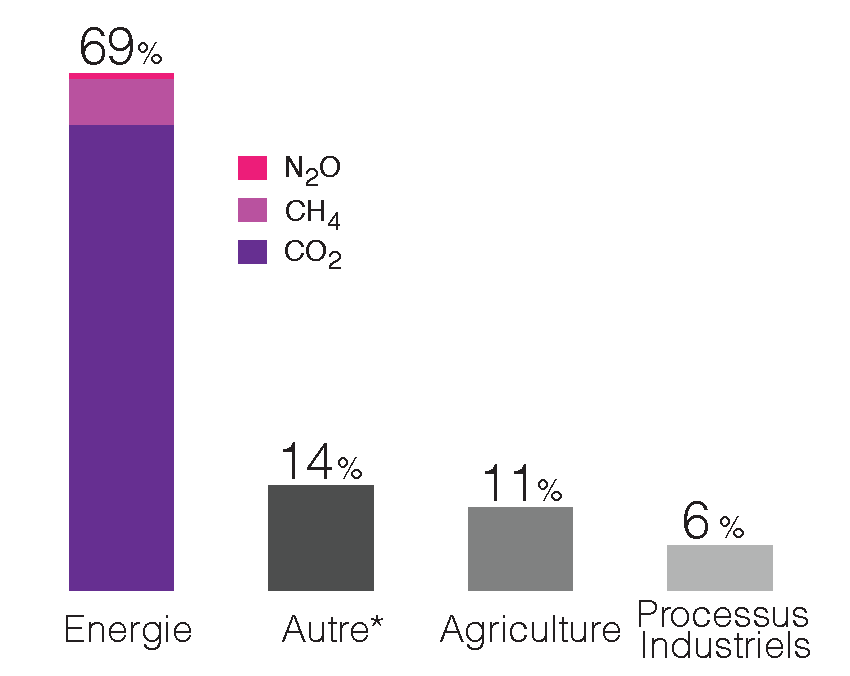
\includegraphics[width=0.7\textwidth]{fig/co2_fossil_fuel_these.pdf}
\caption{Répartitions des GES anthropiques. $^{\ast}$Autre inclut: combustion de
biomasse, émissions indirectes de \ce{N2O} non agricoles, déchets, utilisation
de solvants. Source des données: \citet{IEA_fossil}}
\label{fig:CO2_Fossil}
\end{figure}
\section{Évolution énergétique et scénario de réduction du
\texorpdfstring{\ce{CO2}}{CO2}}
L'Agence internationale de l'énergie (AIE) a publié un rapport dans lequel elle
voit une augmentation de la demande énergétique mondiale de \SI{37}{\percent}
d'ici \num{2040} \citep{WEO2014}. Bien que le choix des politiques et les
évolutions du marché devraient entraîner une baisse de la demande pour les
combustibles fossiles en \num{2040}, ceci ne suffira pas à enrayer
l'augmentation des émissions de dioxyde de carbone, ce qui provoquera une
accélération de la hausse de la température mondiale de \SI{3.6}{\degreeCelsius}
à long terme. Le (GIEC) estime que pour limiter cette hausse à
\SI{2}{\degreeCelsius}, objectif
adopté au niveau international pour prévenir les répercussions les plus graves
du changement climatique, le monde ne devra pas émettre plus de
\SI{1000}{\giga\tonne} \ce{CO2} à compter de \num{2014} \citep{WEO2014}. Les
perspectives en matière de technologies énergétiques \num{2014} \citep{ETP2014}
analysent trois voies possibles pour notre futur énergétique jusqu’en 2050. Le
scénario \SI{6}{\degreeCelsius} (6DS), qui prolonge les tendances actuelles; le
scénario \SI{4}{\degreeCelsius} (4DS), qui reflète les intentions déclarées de
certains pays de réduire les émissions de \ce{CO2} et d'encourager l’efficacité
énergétique et le scénario \SI{2}{\degreeCelsius} (2DS) qui présente un réseau
énergétique durable à faibles émissions de \ce{CO2}.
\begin{figure}[ht]
\centering
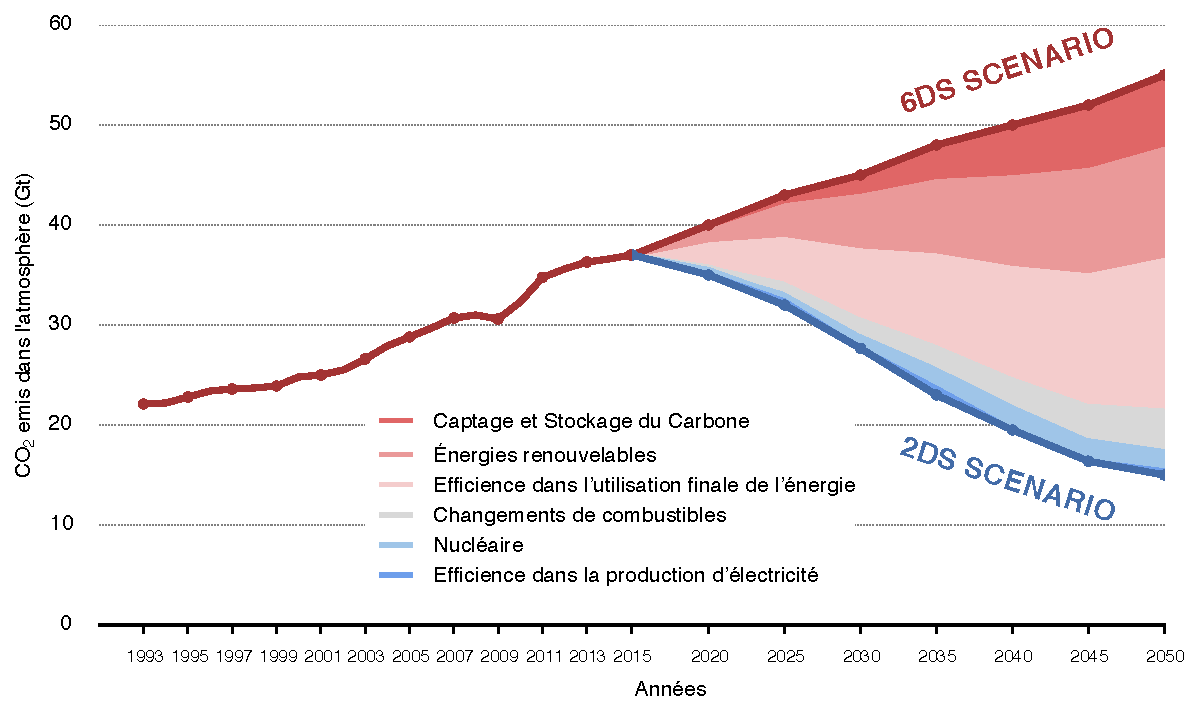
\includegraphics[width=1\textwidth]{fig/EPT2014.pdf}
\caption{Réduction des émissions du \ce{CO2} selon le type de technologie
employée. Source des données: International Energy Agency, Energy Technology
Perspectives 2014 - \url{www.iea.org/etp}}
\label{fig:ETP2014}
\end{figure}
La \cref{fig:ETP2014} montre l'évolution des émissions de \ce{CO2} globale, en
fonction du scénario suivi. Cette figure montre aussi la contribution de chaque
technologie pour atteindre le scénario 2DS, qui permettrait de limiter
l'augmentation de la température globale à \SI{2}{\degreeCelsius}.\\
Les énergies renouvelables connaissent une croissance variable et parmi elles,
l'énergie solaire, l'hydroélectricité et l'éolien terrestre sont les plus
dynamiques surtout dans les économies émergentes qui revoient leurs ambitions à
la hausse et s'affirment comme leaders du déploiement de technologies à faible
empreinte carbone \citep{ETP2014}.\\
En revanche, l'augmentation continue de la consommation de charbon contrecarre
la réduction des émissions résultant des avancées récentes du déploiement des
énergies renouvelables. Ce constat met en lumière la nécessité d'améliorer
l'efficacité des centrales à charbon et d'une utilisation à plus grande échelle
de la technologie du captage et de stockage du carbone (CSC). L'AIE et le GIEC
estiment qu’en \num{2050} environ \SI{14}{\percent} des émissions seront
réduites grâce à l'emploi du CSC. Le CSC n'est cependant pas universellement
populaire parmi les agences de protection de l’environnement et les ONG. En
effet, elle est vue comme une technologie crée par l’industrie pétrolière et
gazière qui leur permettrait de continuer à exploiter et consommer les
ressources énergétiques fossiles comme ils le font actuellement. Cependant, d'un
point de vue pragmatique, cette technologie a le potentiel de mitiger les
émissions globales durant la transition vers de nouvelles technologies à faible
empreinte carbone. Par ailleurs, il y a de nouveaux grands pollueurs comme la
Chine et l'Inde qui sont en pleine expansion économique. Les sociétés
occidentales, qui ont largement profité des énergies fossiles pour leur
développement, sont mal placées pour restreindre la consommation de ces pays.
Donc, le CSC est la seule méthode à court terme qui permettrait d'avoir un
impact significatif sur le bilan carbone.
Il faut se rendre compte que sans la
mise en place de cette technologie à grande échelle, il sera très difficile
d’atteindre les objectifs de réductions demandés par le GIEC. Il faut penser à
développer de plus en plus des projets comme celui de Boundary Dam en
Saskatchewan, où une centrale à charbon a été reconstruite avec une unité de
séquestration et stockage du \ce{CO2}. Cela permet une production
d'électricité de \SI{110}{\MW} tout en assurant une réduction des émissions de
\ce{SO2} et \ce{CO2} de presque \SI{100}{\percent} \citep{WEO2014}.\\
Comme la directrice générale de l'AIE, Maria Van der Hoeven, l'a écrit dans
l'avant-propos du rapport sur le CSC de l'AIE
\citep{IEACCS2013}:\begin{quotation} \emph{Après plusieurs années de recherche,
développements et expériences pratiques importantes, mais limitées, le temps est venu de passer à une vitesse supérieure pour le développement du CSC comme
option énergétique concrète, afin qu'il puisse être déployé à grande
échelle.}\end{quotation}
Cette citation permet de mettre en évidence l'urgence de passer des scénarios à
l'action. Étant donné les tendances passées et actuelles en matière
d’utilisation de combustibles fossiles, il y a une urgence pour le déploiement
du CSC. Cette décennie est cruciale pour faire avancer le CSC au-delà de la phase
démonstrative. Cela signifie que des actions urgentes sont nécessaires, à partir
de maintenant, de la part à la fois de l'industrie et des gouvernements pour
développer des modèles d'affaires et implémenter des cadres incitatifs qui
peuvent entraîner l'application de cette technologie dans le secteur de
l'énergie et d'autres applications industrielles. \par

Bien des gens considèrent le gaz naturel comme un combustible de transition, qui
permettrait de continuer à être dépendant aux combustibles fossiles en réduisant
les émissions de gaz à effet de serre, au cours des prochaines décennies
\citep{Pacala2004}.
Les faibles prix du gaz qui ont accompagné cette augmentation dans la production
ont mené à une croissance dans la demande de gaz. Cette croissance n'a pas été
sans controverse, en particulier dans le cas des gaz de schiste, avec les préoccupations soulevées au sujet de la pollution des
eaux \citep{Osborn2011} et les émissions des gaz à effet de serre (GES), en
particulier ceux liés à la fracturation hydraulique
\citep{Howarth2011a,Howarth2011b}.
\section{Captage et stockage du carbone (CSC)}
Le captage et le stockage du dioxyde de carbone est un processus consistant à
séparer le \ce{CO2} des autres composés industriels et énergétiques, à le
transporter dans un lieu de stockage et à l'isoler de l'atmosphère sur le long
terme \citep{IPCC2005}. Les grandes sources ponctuelles de \ce{CO2} incluent
d'importantes installations faisant appel à des combustibles fossiles (p.ex. les
raffineries et les centrales au charbon), des cimenteries ainsi que les
installations productrices de gaz naturel. Selon les GIEC et l'IEA, le stockage
géologique du \ce{CO2} (piégeage dans des couches réservoirs profondes) est la
seule
technique qui pourrait engendrer des réductions d'émissions de
\SIrange{10}{55}{\percent} à court terme. \\
La \cref{fig:ccs} montre un schéma classique de stockage géologique du
\ce{CO2}. Actuellement il y a plusieurs projets de grande envergure liés à la
séquestration géologique du \ce{CO2}. La \cref{fig:ccs_sites} montre les
principaux projets et leur capacité de stockage annuel.
\begin{figure}[ht]
\centering
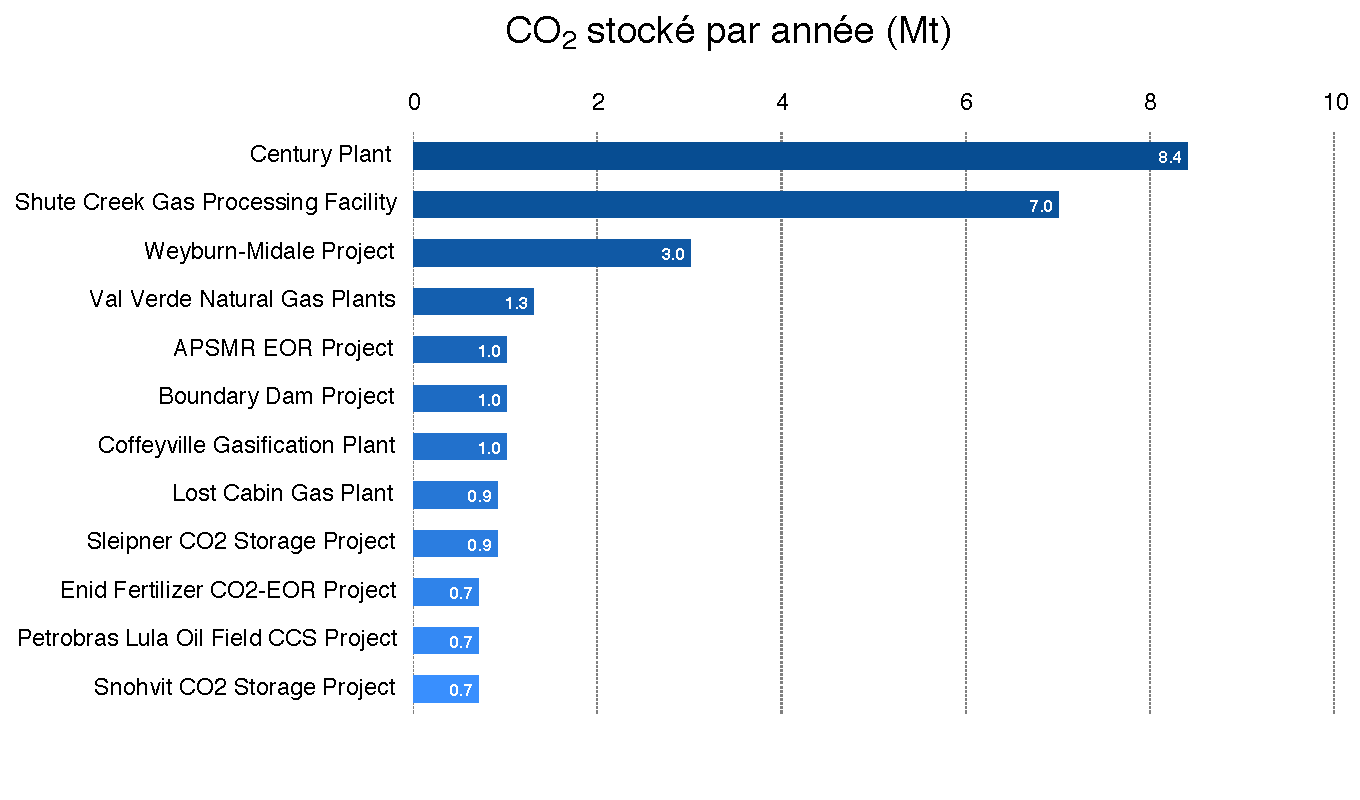
\includegraphics[width=1\textwidth]{fig/CCS_sites.pdf}
\caption{Sites CSC par volume annuel de stockage de \ce{CO2} (mis à jour de
2014). Source des données: \url{http://www.globalccsinstitute.com/}}
\label{fig:ccs_sites}
\end{figure}
Le principe de base derrière ces projets consiste à injecter du \ce{CO2}  à des
pressions d'environ \SI{8}{\mega\pascal} dans un
aquifère salin ou dans un champ de pétrole ou de gaz naturel épuisé situé à une
profondeur supérieure à \SI{800}{\metre}. À ces profondeurs, le \ce{CO2} se
trouve à l'état supercritique avec une densité d'environ
\SI{700}{\kg\per\cubic\meter} qui est plus faible que celle de la plupart des
fluides naturels (saumure ou huile) que l'on trouve dans les réservoirs. C'est
une phase aussi dense qu'un liquide, mais assurant des propriétés de transport
(viscosité et diffusion), proches de celles d'un gaz.\\
Sa flottabilité entraîne la remontée du \ce{CO2} vers la surface jusqu'à ce
qu'il rencontre une couche imperméable capable d’empêcher toute remontée
ultérieure du fluide (aussi appelée couche couverture dans le domaine
pétrolier). Ce phénomène est connu sous le nom de piégeage stratigraphique et on
estime qu’au début de l'injection, la majorité du \ce{CO2} est piégé de cette
façon \citep{Johnson2001}.\\
Par ailleurs, le \ce{CO2} en phase libre se dissout graduellement dans les
fluides résiduels
qui se trouvent dans le réservoir. La dissolution du \ce{CO2} augmente la
densité de la saumure, de sorte que la flottabilité forcera ces fluides vers le
bas en réduisant le risque de fuite. Ce phénomène est connu sous le nom de
piégeage hydrodynamique; \citet{Johnson2001} estiment que jusqu'à
\SI{15}{\percent} du \ce{CO2} peut être stocké de cette façon.\\
Le \ce{CO2} libre et la saumure enrichie de \ce{CO2} se trouvent en déséquilibre
chimique avec les roches du réservoir; des réactions chimiques qui produisent de
la dissolution ou de la précipitation auront donc lieu. Le scénario optimal est
celui où les minéraux qui contiennent des carbonates précipitent. Ce phénomène
est connu sous le nom de piégeage minéral. Cependant, le taux de précipitation
pour ce processus est très lent donc sur une échelle de temps décennale,
seulement une faible quantité (\SI{<1}{\percent}) de \ce{CO2} sera piégée de
cette façon. \citep{Johnson2001}.
\begin{figure}[ht]
\centering
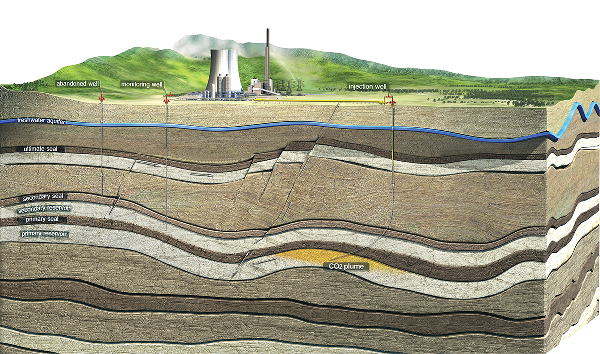
\includegraphics[width=1\textwidth]{fig/ccs.pdf}
\caption{Schéma représentant le stockage géologique du \ce{CO2}. Source de
l'image: \url{http://www.dnv.com}}
\label{fig:ccs}
\end{figure}
\subsection{Réservoirs d'hydrocarbure épuisés}
La pression des réservoirs d'hydrocarbures épuisés chute et les hydrocarbures qui étaient contenus dans les pores et les fractures
sont graduellement remplacés par les fluides de la formation, généralement de la saumure.
Depuis les années 1960, une pratique courante en ingénierie de réservoir est
celle d'injecter de la saumure pour maintenir une pression élevée. Dans certains
cas, le \ce{CO2} a été utilisé à la place de la saumure. En effet, il a été
découvert qu'en injectant du
\ce{CO2} on est capable d’augmenter l'extraction d'hydrocarbures tout en
assurant que le \ce{CO2} injecté reste en place. Ce type de stockage est
actuellement mené dans le projet de Weyburn-Midal en Saskatchewan. Il y a trois
avantages principaux à stocker le \ce{CO2} de cette façon. Premièrement, le
bénéfice économique est accru en raison d'une augmentation de l'extraction
d'hydrocarbures.
Deuxièmement, les réservoirs sont très bien étudiés et les volumes potentiels de
stockage sont connus. Finalement, la majorité des infrastructures nécessaires
sont déjà en place.\\
Cependant, il faut considérer que les puits abandonnés pourraient fournir une
voie préférentielle pour la remontée du \ce{CO2} vers la surface et que les
activités d'extraction pourraient avoir endommagé la roche couverture.
\subsection{Aquifères salins}
Le \ce{CO2} est un liquide de faible densité; il est donc piégé dans des
réservoirs poreux qui sont recouverts par une couche imperméable. Ce type de
piège stratigraphique est abondant dans la plupart des bassins sédimentaires
où les roches sont saturées en saumure. Ces aquifères salins représentent de
loin le plus grand volume disponible pour le stockage du \ce{CO2}.
\citet{Bedard2013} estiment que les aquifères salins des Basses-Terres du
St Laurent (Québec, Canada) renferment un potentiel de stockage d'environ
\SI{3}{\giga\tonne} de \ce{CO2}, ce qui représenterait les émissions de toute
la
province de Québec pendant \num{150} ans. Cependant, les aquifères salins
n'ayant aucune valeur commerciale, ils ne sont pas très bien étudiés et il est
donc
difficile d'obtenir des estimations précises ainsi que des données fiables pour
assurer la sécurité du stockage. Actuellement, il existe trois projets
importants dans ce type d'environnement, soit à Sleipner et Sn{\o}hvit, dans la
mer du Nord, et Aquistore en Saskatchewan, où la viabilité du projet de stockage
dans des aquifères
salins à été démontrée.
\section{La zone d'étude}
\label{sc:site_etude}
Le Ministère du Développement durable, de I'Environnement et des Parcs (MDDEP)
du Québec a octroyé une subvention à I'INRS-ETE pour mettre en place une chaire
de recherche sur la séquestration géologique du \ce{CO2} au Québec. Des
aquifères salins profonds ont été identifiés à plusieurs niveaux
stratigraphiques dans la région de Bécancour, entre Montréal et Québec: les
calcaires du Groupe de Trenton, les grès dolomitiques du Groupe de Beekmantown
(Formation Theresa) et les grès quartzeux du Groupe de Potsdam (Formations
Cairnside et Covey Hill). Ces aquifères sont situés à une profondeur moyenne
allant de \SIrange{795}{1230}{\metre} \citep{INRS1}. \\
Les travaux de recherche de la chaire ont montré que les épaisseurs nettes des
intervalles productifs sont plus importantes dans les grès du Groupe du Potsdam
et particulièrement dans les grès de la Formation Covey Hill (\SI{196}{\metre}).
Les grès de Covey Hill ont aussi les porosités effectives les plus importantes
(\SI{6}{\percent}), les perméabilités de la matrice les plus élevées
(\SI{2.4e-16}{\metre\squared}) ainsi qu'une salinité relativement faible
(\SI[per-mode=symbol]{108.500}{\milli\gram\per\litre}) \citep{TranNgoc2014}. Les
grès de la Formation Cairnside ont aussi un potentiel de stockage intéressant. Cependant leur faible porosité et perméabilité ainsi que leurs
eaux fortement salines sont moins favorables pour le stockage du \ce{CO2}. Les
\cref{fig:map,fig:strati} de l'\cref{ch:article1} à la \cpageref{fig:strati}
montrent les bassins sédimentaires de la zone d'études et la stratigraphie
simplifiée des Basses-Terres du St Laurent respectivement. \\
Dans ce travail, les aquifères du Groupe du Potsdam ont été choisis comme
réservoir cible pour la séquestration géologique du \ce{CO2} au Québec  pour leurs propriétes réservoirs mentionnées ci-haut. La
description des propriétés physiques des échantillons du Covey Hill et du
Cairnside sont présentés dans le \cref{tbl:prop} de l' \cref{ch:article1} à la
\cpageref{tbl:prop}.
\section{Objectifs de la thèse}
Pour que le captage et stockage du \ce{CO2} aient un impact positif sur
l'environnement, le \ce{CO2} doit donc être stocké dans le sous-sol aussi
longtemps qu'il le faut pour que les émissions anthropologiques chutent à des
niveaux acceptables et que le cycle du carbone se rétablisse et se stabilise.
Ces contraintes nécessitent que le \ce{CO2} soit stocké sur une échelle de temps
de l'ordre de \numrange{e1}{e4} ans. Pour atteindre cette exigence, on doit
s'assurer que le \ce{CO2} reste en place et ne puisse migrer sur de grandes
distances ni verticalement ni horizontalement. \\
Ceci nous oblige à répondre à deux questions scientifiques principales pour que
les projets de  CSC deviennent économiquement et politiquement acceptables:
\begin{enumerate}[-]
\item Peut-on utiliser les méthodes géophysiques pour surveiller la migration du
\ce{CO2} dans un contexte de faible porosité et perméabilité comme celui des
Basses-Terres du St Laurent?
\item Peut-on utiliser les données géophysiques afin de quantifier l'étalement
du panache de \ce{CO2} dans le sol et quantifier son incertitude?
\end{enumerate}
L'objet de cette thèse est donc d'analyser et répondre à ces questions afin de
renforcer les bases scientifiques pour le stockage du \ce{CO2} dans l'aquifère
salin des Basses-Terres du St Laurent (BTSL), identifié comme cible principale
pour le développement du CSC dans la province du Québec.
\subsection{Peut-on utiliser les méthodes géophysiques pour surveiller la
migration du \texorpdfstring{\ce{CO2}}{CO2} dans un contexte de faible
porosité et perméabilité comme celui de Basses-Terres du St Laurent?}
\label{sc:obj1}
La surveillance sismique temporelle a prouvé être une méthode
efficace pour aider à la gestion des réservoirs d'hydrocarbures depuis les
années 1990 \citep{Johnston2010}. Plus récemment, cette technique a été adoptée
à des fins de surveillance des sites de stockages de \ce{CO2} où l'objectif est
non seulement celui de surveiller le réservoir, mais aussi de sonder et
quantifier l’intégrité de la roche couverture. Cette technique a été utilisée à
Sleipner \citep{Arts2004} à Weyburn-Midale (Canada) \citep{Li2001,Davis2003,White2013} à
In Salah (Algerie) et Sn{\o}hvit (Norvège) \citep{Eiken2011} et dans le projet Aquistore (Saskatchewan) \citep{Roach2015} ainsi
que dans plusieurs projets pilotes tels que Cranfield (États-Unis) \citep{Zhang2012}, Otway (États-Unis)
\citep{Urosevic2010}, Nagaoka (Japon) \citep{Sato2011} et Ketzin (Allemagne)
\citep{Luth2011,Ivanova2012}. Dans l'ensemble, ces sites présentent des
conditions d'injection idéales avec des porosités de \SIrange[range-units =
single]{15}{20}{\percent} et des perméabilités de \SIrange[range-units =
single]{5e-12}{5e-14}{\metre\squared}.  \\
Dans le cas de la surveillance du \ce{CO2}, une des limitations majeures de la
sismique de surface, est sa résolution verticale. En effet, il est très
difficile, voire impossible, d’imager des couches plus minces que
\SIrange{10}{15}{\metre}, aux profondeurs des réservoirs ayant un potentiel de
stockage \citep{Arts2004}. Cependant, dans des environnements stratifiés, il
n'est pas rare que le \ce{CO2} reste piégé dans des couches plus minces que la
limite de résolution de la sismique de surface
\citep{Chadwick2004,Chadwick2005,Chadwick2009,Bickle2007,Lippard2008}. Le
profilage sismique vertical (PSV) pourrait partiellement résoudre le problème de
résolution. Cette méthode présente l'avantage de placer des géophones dans un
puits, au niveau du réservoir en améliorant le pouvoir de résolution. Cette
technique a été employée avec succès pour la surveillance de l'injection d'une
petite quantité de \ce{CO2} dans la Formation de Frio au Texas \citep{Daley2008}
ainsi que pour la surveillance temporelle du \ce{CO2} à Ketzin en Allemagne.
\textbf{Un des objectifs de cette thèse est donc celui de tester un modèle
numérique pour le PSV comme outil de surveillance de la propagation du \ce{CO2}
dans des conditions de très faible porosité (\SIrange[range-units =
single]{4}{6}{\percent}) et perméabilité (\SIrange[range-units =
single]{1.2e-16}{2.5e-16}{\metre\squared}).}\par

Dans les approches conventionnelles, en raison du nombre limité de puits et de
l'absence de méthode éprouvée
d'assimilation quantitative de données indirectes, les modèles géologiques
utilisés pour la modélisation sismique sont très simplistes, homogènes et ne
reflètent pas la réalité \citep{DubreuilBoisclair2012,Claprood2013}. De plus,
les algorithmes utilisés pour la propagation des ondes sismiques dans un milieu
poreux
ne tiennent pas compte de l'influence des fluides. \citet{Giroux2012} présente
une implémentation des CPML (\emph{convolutional perfectly matched layer}) pour
les milieux poroviscoélastiques isotropes et anisotropes. L'approche
poroviscoélastique est peut-être l'outil le plus efficace pour étudier l’effet
des
fluides saturant les roches, car leurs propriétés sont directement prises en
compte dans les équations. \textbf{Un autre objectif est donc de
construire un modèle géologique stochastique de référence afin de produire des
sismogrammes en utilisant une formulation poroviscoélastique. Des mesures de
laboratoires ont été nécessaires afin d’étalonner le modèle géologique.}\par

La modélisation de la réponse sismique à l'injection du \ce{CO2} nécessite des
modèles représentatifs pour prédire correctement le comportement des ondes
acoustiques traversant des milieux géologiques complexes.
Cela implique la modélisation de l'écoulement du fluide afin de prédire la
progression du panache de \ce{CO2} dans le réservoir. L'approche classique
repose sur l'utilisation des méthodes numériques en trois dimensions pour
résoudre le système avec un degré de précision élevé. Toutefois, cela implique
des efforts importants de calcul, qui ne sont pas toujours abordables ou même
possibles à mettre en oeuvre. Au cours des dernières années, des approches
employant des méthodes semi-analytiques ont été mises au point
\citep{Nordbotten2005a, Nordbotten2009}. Un outil de simulation prometteur pour
la modélisation rapide et précise de la séquestration de \ce{CO2} est basé sur
l'hypothèse d'équilibre vertical (VE). Au cours des dernières années, les
méthodes VE ont été employées pour simuler l'injection et la migration du
\ce{CO2} à grande échelle, pour laquelle l'hypothèse d'équilibre vertical avec
interface nette entre \ce{CO2} et saumure peut être formulée
\citep{Nordbotten2005a,Celia2006,Nordbotten2006}. \textbf{Finalement, le dernier
objectif de cette section est de modéliser l'injection et la migration du
\ce{CO2} avec l'hypothèse d'équilibre vertical afin de pouvoir tester le PSV
comme outils de surveillance temporelle.}
\subsection{Peut-on utiliser les données géophysiques afin de quantifier
l'étalement du panache de \texorpdfstring{\ce{CO2}}{CO2} dans le sol et
quantifier son incertitude?}
\label{sc:obj2}
Tout processus d'évaluation des ressources de stockage géologique du \ce{CO2}
nécessite des estimations de la quantité de \ce{CO2} qui peut être stockée dans
le sous-sol. Les incertitudes liées à cette estimation dépendent entre autres de
la compréhension du sous-sol en terme de données géologiques et des modèles. De
manière générale, en raison du faible nombre de données, un seul modèle
déterministe est utilisé pour évaluer la ressource d'un site de stockage du
\ce{CO2}. Cependant, étant donné que notre connaissance du sous-sol est toujours
très limitée, le modèle déterministe ne sera jamais assez fidèle à la réalité.
Finalement, on ne fournit qu'un seul modèle qui est certain d'être non réaliste
tout en négligeant l'incertitude. Cette situation peut être améliorée en
utilisant des méthodes probabilistes qui respectent l'incertitude des données
que l'on peut exploiter tant dans la construction du modèle statique (porosité,
perméabilité) que pour le suivi et l'évaluation de l'injection. De plus, dans
les cas d'injection de fluides, il est important d’intégrer la surveillance
temporelle sismique avec les simulations d’écoulement de \ce{CO2} dans un cadre
commun appelé calage historique \citep{Doyen2007}. Cette pratique est
assez bien connue dans le domaine pétrolier et gazier, mais elle n'a pas encore
été adoptée dans la séquestration et stockage du \ce{CO2}. De plus, dans le cas
de la CSC, il n'y a pas d'information directe sur le mouvement du panache, car,
dans la plupart du temps, il n'y a qu'un seul puits de surveillance.
\textbf{Un autre objectif de
la thèse est donc de définir une séquence logique de modélisation stochastique
d'un réservoir potentiel pour la séquestration géologique du \ce{CO2}. Afin de
valider l'adéquation optimale des modèles, ceux-ci sont testés en fonction de leur
réponse sismique poroviscoélastique par rapport aux données mesurées.}

%!TeX root = Thesis_LP.tex
\chapter{La sismique comme outil de surveillance du
\texorpdfstring{\ce{CO2}}{CO2}}
\label{ch:sismique}
Cette section décrit brièvement les bases théoriques et les démarches
méthodologiques nécessaires pour répondre au premier objectif de l’étude. La
\cref{sc:theorie_sismique} présente la base théorique de la propagation des
ondes acoustiques dans les milieux poreux. Les détails de la méthodologie
utilisée se retrouvent dans l’article I faisant partie de cette thèse. Afin
d'éviter la redondance, les \cref{sc:laboratoire,,sc:model} présentent un survol
sur la méthodologie utilisée pour les mesures de laboratoires et pour la
modélisation sismique de l'injection du \ce{CO2} et une discussion sur les
résultats.
% \section{La sismique comme outil de surveillance du
% \texorpdfstring{\ce{CO2}}{CO2}}
% \label{sc:sismique}
\section{Concepts théoriques de base}
\label{sc:theorie_sismique}
\subsection{Les milieux élastiques}
 On appelle onde sismique toute onde mécanique qui traverse un milieu
géologique. Dans l'analyse des données sismiques, on utilise souvent
l'approximation d'élasticité, c'est à dire que les particules reviennent à leur
place après le déplacement imposé par l'onde mécanique.\\
La théorie de l'élasticité part du principe que si un solide est soumis à des
contraintes, il se déforme et lorsque la contrainte est retiré il reprend sa
forme initiale. En sismique, on impose a priori que forces et déformations
sont minimes et donc que les relations entre forces et déformations sont
linéaires, ce qui permet de représenter le milieu comme parfaitement élastique
où toute l'énergie est conservé \citep{Sheriff1995}. Il existe deux types de
contraintes, définis par l’orientation selon lesquelles la force est exercée. Si
la force est appliquée perpendiculairement à la surface, on parle de contrainte
normale, si elle est appliquée de façon tangentielle, on parle de contrainte de
cisaillement. Le comportement mécanique d’un milieu élastique, anisotrope et
linéaire peut être décrit par la loi de Hooke généralisée:
\begin{equation}
\sigma_{ij} = C_{ijkl}*\epsilon_{kl} \qquad i,j,k,l = 1,2,3
\label{eq:hooke}
\end{equation}
où $\sigma$ représente la contrainte, $C$ est le tenseur de rigidité de la
matrice et $\epsilon$ est la déformation.
La contrainte et la déformation peuvent être representée par des matrices $3
\times 3$ (9 composantes) qui représentent la tridimensionnalité d’un volume. Le
comportement du milieu peut donc être modélisé par un tenseur de rigidité de
81 composantes ($3 \times 3 \times 3 \times 3$) qui sont réduites à 21 grâce à
la symétrie entre la contrainte et la déformation. Il s’agit du nombre maximal
de composantes qu’un milieu homogène linéaire peut avoir. Un milieu isotrope,
qui présente la symétrie maximale, est caractérisé par deux composantes
indépendantes, tandis que les milieux avec une symétrie triclinique sont
représentés par l'ensemble des 21 composantes.\par

C’est une pratique courante d’utiliser la notation de Voigt pour représenter les
contraintes, les déformations et les tenseurs de rigidité. Avec cette notation,
les contraintes et les déformations deviennent des vecteurs de six éléments
plutôt que des matrices carrées de 9 éléments. Avec la notation de Voigt, les 4
indices du tenseur de rigidité sont réduits à deux, en utilisant la convention
suivante:\par
$$\begin{matrix}
ij(kl) & I(J)\\
 11 & 1 \\
 22 & 2 \\
 33 & 3 \\
 23, 32 & 4 \\
 13, 31 & 5 \\
 12, 21 & 6 \\
\end{matrix}$$
En utilisant la notation de Voigt, on peut écrire l’\cref{eq:hooke} sous cette
forme:
\[
    \begin{bmatrix}
        \sigma_{1} \\
        \sigma_{2} \\
        \sigma_{3} \\
        \sigma_{4} \\
        \sigma_{5} \\
        \sigma_{6} \\
    \end{bmatrix}
    =
    \begin{bmatrix}
        C_{11} & C_{12} & C_{13} & C_{14} & C_{15} & C_{16} \\
        C_{12} & C_{22} & C_{23} & C_{24} & C_{25} & C_{26} \\
        C_{13} & C_{23} & C_{33} & C_{34} & C_{35} & C_{36} \\
        C_{14} & C_{24} & C_{34} & C_{44} & C_{45} & C_{46} \\
        C_{15} & C_{25} & C_{35} & C_{45} & C_{55} & C_{56} \\
        C_{16} & C_{26} & C_{36} & C_{46} & C_{56} & C_{66} \\
    \end{bmatrix}
    \begin{bmatrix}
        \epsilon_{1} \\
        \epsilon_{2} \\
        \epsilon_{3} \\
        \epsilon_{4} \\
        \epsilon_{5} \\
        \epsilon_{6} \\
    \end{bmatrix}
.\]
Dans le cas isotrope, la matrice de rigidité s’écrit comme suit:
\[
    \begin{bmatrix}
        C_{11} & C_{12} & C_{12} &   0    &   0    &    0   \\
        C_{12} & C_{11} & C_{12} &   0    &   0    &    0   \\
        C_{12} & C_{12} & C_{11} &   0    &   0    &    0   \\
           0   &   0    &   0    & C_{44} &   0    &    0   \\
           0   &   0    &   0    &   0    & C_{44} &    0   \\
           0   &   0    &   0    &   0    &   0    & C_{44} \\
    \end{bmatrix}
, \qquad C_{12} = C_{11} - 2C_{44}
\]
Les relations entre les constantes élastiques $C$  et les paramètres de Lamé
$\lambda$ et $\mu$ pour un milieu isotrope sont:
\begin{equation}
C_{11} = \lambda + 2\mu = K + \frac{4}{3}\lambda, \qquad C_{12} = \lambda,
\qquad C_{44}= \mu,
\end{equation}
où $K$ est le \textbf{module d'incompressibilité} et $\lambda$ le \textbf{module
de cisaillement} du milieu.
En sismique, la propagation des ondes est généralement donnée en termes de module
d'incompressibilité et de cisaillement car ils ont des interprétations physiques
claires. Le premier est essentiellement la mesure de la résistance du milieu à
une compression uniforme (rigidité). Le module de cisaillement, ou deuxième
paramètre de Lamé est une mesure de la résistance du milieu à une déformation en
cisaillement. Le premier paramètre de Lamé, $\lambda$, n'a aucune interprétation
physique, mais il intervient dans la simplification de la matrice de rigidité.\par
D'autres modules peuvent être utilisés pour décrire un milieu isotrope sous une
contrainte uniaxiale. Le \textbf{module de Young} $E$ est le rapport entre la
contrainte appliquée et l'allongement relatif. Le \textbf{coefficient de
Poisson} est le rapport entre la déformation transversale et axiale. Dans le cas
d'une déformation uniaxiale, on peut utiliser le \textbf{module des ondes P}
défini comme le rapport entre la contrainte et la déformation axiale. Pour de
plus amples détails sur le sujet des milieux élastiques voici quelques
références: \citet{Bourbie1986,Carcione2007,Mavko2009}
\subsection*{La propagation des ondes dans les milieux élastiques}
\label{sc:prop_ondes}
Dans la section précédente, la relation entre contrainte appliquée et
déformation a été établie en utilisant la loi de Hooke. Cependant, cette loi ne
donne pas la variation du déplacement des points du milieu avec le temps. La
propagation d’une onde dans l’espace et dans le temps peut être décrite si le
volume du milieu considéré n’est pas en équilibre statique. La deuxième loi du
mouvement de Newton indique qu’une force non nulle exercée sur un corps est
égale au produit de la masse et de l’accélération du corps. En incluant la loi
de Hooke dans l’équation du mouvement et en exprimant la déformation en terme de
déplacement, l’équation d’onde à une dimension dans un milieu élastique pour un
déplacement $u$ est donnée par:
\begin{equation}
\rho\frac{\partial^2 u}{\partial t^2} = C\nabla^2u,
\label{eq:onde}
\end{equation}
où $u$ est fonction de la position et du temps, $\rho$ est la
densité\footnote{À strictement parler il s'agit de la masse volumique, mais en
géophysique on utilise couramment le terme de densité.} du milieu
élastique et $C$ et la constante de rigidité ou module élastique relatif au
type d'onde pris en considération. La vitesse de l'onde pour le cas le plus
général de l'\cref{eq:onde} est:
\begin{equation}
V = \sqrt{\frac{C}{\rho}}
\label{eq:velocity_gen}
\end{equation}
Essentiellement, l’équation d’onde met en relation la dérivée dans le temps avec
la dérivée dans l’espace du déplacement par la constante de proportionnalité de
$V^2$.\\
Dans un milieu homogène isotrope, il y a 2 types d’ondes principales qui sont
étudiées: les ondes de compression $P$ et les ondes de cisaillement $S$. Pour la
vitesse des ondes $P$ et $S$, l'\cref{eq:velocity_gen} devient:
\begin{equation}
V_p = \sqrt{\frac{C_{11}}{\rho}} = \sqrt{\frac{\lambda + 2\mu}{\rho}} =
\sqrt{\frac{K+\frac{4}{3}\mu}{\rho}}\quad et
\label{eq:vitesse_p}
\end{equation}
\begin{equation}
V_s = \sqrt{\frac{C_{44}}{\rho}} = \sqrt{\frac{\mu}{\rho}} ,
\label{eq:vitesse_s}
\end{equation}
respectivement. Les fluides ne peuvent pas soutenir les forces de cisaillement,
le module de cisaillement des fluides est donc égal à zéro. Seules les ondes
$P$ peuvent voyager dans des liquides dont la vitesse de l’onde est:
\begin{equation}
V_p = \sqrt{\frac{K}{\rho}} .
\label{eq:velocity_pliq}
\end{equation}
La théorie présentée jusqu'ici s'applique à des milieux monophasiques (solides).
Pour de plus amples détails sur la propagation des ondes dans ce type de milieu,
voici quelques références: \citet{Sheriff1995,Aki1980}.\par

Pour étendre l'étude de la propagation des ondes aux milieux poreux saturés
des fluides, on peut appliquer le modèle de Biot \citep{Biot1956a,Biot1956b}. Dans ce
modèle, les interactions fluide-structure sont prises en compte à travers trois
types de couplage : les couplages massiques, élastiques et visqueux.
\subsection{Les milieux viscoélastiques}
Le comportement viscoélastique est une réponse mécanique, en fonction du temps,
d'un milieu à des variations des contraintes appliquées. \citet{Boltzmann1874} a
été parmi les premiers scientifiques à introduire le concept de mémoire: pour un
point donné d'un milieu, la contrainte appliquée au temps $t$ dépend de la
déformation du milieu au temps $t-1$. Différemment d'un milieu purement
élastique, où l'énergie utilisée pour déformer le milieu est conservée, dans un
milieu viscoélastique, elle est partiellement dissipée. N'ayant plus d'énergie
pour retourner jusqu'à l'état initial, un milieu viscoélastique reste donc déformé
\citep{Carcione2007}. \\
Le facteur adimensionnel de qualité $Q$ permet de caractériser la dissipation
d'un milieu. Par définition, le facteur Q est inversement proportionnel à
l’énergie absorbée par le milieu lors d’un cycle d’oscillation de l’onde
\citep{Sheriff1995}.  Cette définition revêt la forme
mathématique suivante:
\begin{equation}
Q = \dfrac{2\pi}{\Delta E /E}.
\label{eq:facteur_Q}
\end{equation}
Ainsi, plus le matériau est de piètre qualité du point de vue sismique, plus
l’énergie de l’onde sismique dissipée ($\Delta E$) est grande, plus le facteur
de qualité sera faible \citep{Giroux2001}. Pour un système viscoélastique, il y
a une relation directe entre la vitesse de dispersion et le facteur de qualité.
\subsection{Les milieux poroviscoélastiques}
Le concept de viscoélasticité peut être introduit dans les équations de Biot
\citep{Biot1956a,Biot1956b} pour la modélisation des mécanismes d'atténuation
liée à l'énergie de déformation (dissipation due à la rigidité) et à l'énergie
cinétique (dissipation viscodynamique) \citep{Carcione2007}.
\citet{Carcione1998} a modifié les équations de Biot afin d'inclure des
mécanismes d'interaction matrice-fluide à travers les fonctions de relaxation
viscoélastique. Cette formulation est la plus appropriée pour décrire le
phénomène de l'injection du \ce{CO2} dans des grès, car il permet d’inclure les
propriétés des fluides dans les équations de propagation des ondes.\\
Les développements mathématiques pour la propagation des ondes dans les milieux
viscoélastiques et poroviscoélastiques sont détaillés dans \citet{Bourbie1986}
et \citet{Carcione2007}
\subsection{La physique des roches}
La discipline de la physique des roches a comme objectif d'établir des relations
entre les propriétés physiques des roches et leur réponse géophysique mesurée. Dans notre cas,
la physique des roches étudie les propriétés physiques qui influencent la
propagation des ondes sismiques à travers les roches, à savoir la
compressibilité, la rigidité, la porosité, la densité et les fluides
interstitiels. Pour établir ces relations, il faut connaître les propriétés
élastiques de la matrice et des fluides interstitiels ainsi que les modèles
d'interaction entre fluide et roche. \\
Le concept de substitution de fluide se réfère à la modélisation des vitesses
des ondes sismiques dans un milieu poreux saturé, en faisant varier les propriétés physiques des fluides intersticiels.
\subsubsection{L'équation de Gassmann}
En physique des roches, la relation de Gassmann \citep{Gassmann} est fréquemment
utilisée en raison de sa simplicité et de son applicabilité dans la gamme des fréquences
sismiques, autour de \SI{100}{\hertz} \citep{Mavko2009}. Dans sa formulation,
Gassmann, fait plusieurs hypothèses:
\begin{enumerate}
\item La roche est considérée comme homogène et isotrope;
\item Les minéraux constituant la roche ont le même module de rigidité et de
cisaillement;
\item Les fluides interstitiels peuvent circuler librement et les pores sont
connectés entre eux;
\item Les pores sont complètement saturés;
\item Les fluides interstitiels n'interagissent pas avec les minéraux formant la matrice rocheuse;
\item Les fréquences sont suffisamment basses pour que la pression induite dans
les pores puisse se rééquilibrer.
\end{enumerate}
Dans l’équation de Gassmann, le module de la roche saturée $K$ est relié au
module de la matrice (roche sèche) $K_{dry}$, le module de la roche solide
(minéraux constituant la roche) $K_s$, le module du fluide interstitiel $K_f$ et
la porosité de la roche $\phi$ par \citep{Mavko2009}:
\begin{equation}
\dfrac{K}{K_s - K} = \dfrac{K_{dry}}{K_s - K_{dry}} + \dfrac{K_f}{\phi (K_s -
K_f)},
\label{eq:gass}
\end{equation}
en réarrangeant l'\cref{eq:gass}, on a:
\begin{equation}
K = K_{dry} + \dfrac{\bigg(1 -
\dfrac{K_{dry}}{K_s}\bigg)^2}{\dfrac{\phi}{K_f}+\dfrac{1-\phi}{K_s} +
\dfrac{K_{dry}}{K_s^2}}.
\label{eq:gasmmann}
\end{equation}
Si le module de la roche sèche $K_{dry}$ n'est pas disponible, le module de la
roche saturée  $K$ peut être lié au module de la roche saturée avec un autre
fluide $K_2$ selon la relation suivante\citep{Mavko2009}:
\begin{equation}
\dfrac{K}{K_s - K} - \dfrac{K_{f}}{\phi(K_s - K_{f})} = \dfrac{K_2}{K_s - K_2} -
\dfrac{K_{f2}}{\phi(K_s - K_{f2})}.
\end{equation}
Dans la formulation de Gassmann, le module de cisaillement est indépendant des
fluides qui saturent la roche, car ces derniers sont incapables de soutenir des
forces de cisaillement. Donc, le module de cisaillement de la roche saturée est
égal au module de cisaillement de la roche sèche:
\begin{equation}
\mu_{sat} = \mu_{dry}
\end{equation}
À partir des résultats de $K$ et $\mu$, les vitesses $V_p$ et $V_s$
correspondantes peuvent être calculées en utilisant les
\cref{eq:vitesse_p,,eq:vitesse_s} où la densité de la roche saturée est:
\begin{equation}
\rho_{sat} = (1-\phi)\rho_s + \phi \rho_f.
\end{equation}
Avant d'effectuer la substitution de fluide en utilisant l'\cref{eq:gasmmann},
il faut déterminer la porosité ($\phi$), les propriétés des fluides
interstitiels ($K_f$, $\rho_f$), le module de la matrice ($K_{dry}$) ainsi que le
module des solides ($K_s$) de la roche. Ces quatre composantes peuvent être
inférées à partir des mesures de laboratoire ou par l'analyse de diagraphies en forage. Une
revue exhaustive des méthodes permettant de déterminer $\phi$, $\rho_f$, $K_f$, $K_{dry}$, $K_s$ se trouve dans
\citet{Smith2003} et \citet{Mavko2009}.
\subsubsection{La formulation de Biot}
Contrairement à Gassmann, Biot prédit la dépendance en fréquence des vitesses
des ondes dans les milieux saturés. Il a présenté sa théorie pour les basses et
les hautes fréquences dans \citet{Biot1956a,Biot1956b}. Pour les basses
fréquences, la relation de Biot se réduit à celle de Gassmann. Les mêmes
hypothèses que pour Gassmann s'appliquent. De plus, Biot suppose que les fluides
interstitiels sont newtoniens (c'est-à-dire que loi contrainte – vitesse de déformation est linéaire, et où la constante de proportionnalité est la viscosité). Dans sa formulation, Biot représente la
dépendance en fréquence des ondes en incorporant les interactions visqueuses et
inertielles entre le fluide interstitiel et la matrice solide de la roche. \\
Pour les hautes fréquences, les fluides interstitiels n'ont pas assez de temps
pour se rééquilibrer donnant naissance à des phénomènes d’atténuation et
dispersions connus sous le nom d'écoulement de fluide induit par la propagation
des ondes, de l'anglais \emph{wave-induced fluid flow} \citep{Muller2010}.\\
Les bases mathématiques de la formulation de Biot sont développées dans les
articles originaux \citet{Biot1956a,Biot1956b} ainsi que dans
\citet{Bourbie1986}, \citet{Carcione2007} et \citet{Allard2009}.
\section{Mesures sismiques de laboratoire avec injection de
\texorpdfstring{\ce{CO2}}{CO2}}
\label{sc:laboratoire}
La première étape de ma thèse a été de vérifier et de mesurer la relation entre
les propriétés physiques et géologiques dans les conditions de pression et
température des réservoirs potentiels du Québec. Les mesures ont été
 effectué un stage de 3 mois dans le laboratoire du professeur Schmitt à
l'Université d'Edmonton.
La méthode de la transmission par impulsion est parmi les méthodes ultrasoniques
les plus utilisées en physique des roches \citep{Wyllie1958,Nur1971,Timur1977,Toksz1979,Tosaya1982,Blair1990,Wang1991,Cadoret1995,Adam2006,Verwer2008,Yam2011,Njiekak2013,Schmitt2015}
et elle est la seule méthode appliquée à ce jour pour les études en laboratoire
du \ce{CO2} sur les ondes élastiques. En comparaison avec d'autres techniques,
la transmission par impulsion est relativement simple et facilement applicable.
Des variables telles que la pression, la température et la saturation peuvent
être manipulées pour étudier leur effet sur la réponse sismique. \\
L'approche proposée dans cette étude s'inspire directement de
\citet{Schmitt2015} et les réponses sismiques associées aux différentes phases
du \ce{CO2} ont été étudiées sur deux échantillons, un du Covey Hill et un du Cairnside,
complètement saturés en \ce{CO2} avec la méthode de transmission par impulsion.
Avec cette méthode, l'échantillon est placé entre la source et un récepteur qui
sont généralement des transducteurs piézoélectriques en céramique. La
\cref{sc:art_1_ultrasonic_measurements} de l'article I à la
\cpageref{sc:art_1_ultrasonic_measurements} décrit la procédure des mesures de
laboratoire, de la préparation des échantillons jusqu'aux analyses. Les
paragraphes qui suivent donnent un aperçu des étapes principales.
\subsection{Préparation des échantillons}
Deux échantillons cylindriques, de \SI{3.7}{\cm} et de \SI{4}{\cm} de longueur,
ont été préparés pour les analyses. Un aspect très important pour améliorer la
transmission du signal et pour minimiser les erreurs de mesure est de s'assurer
que les extrémités de l'échantillon soient les plus parallèles possible entre
elles. Les échantillons ont été initialement taillés afin de les rendre
approximativement parallèles et ensuite ont été polis en utilisant une meuleuse
afin que le parallélisme entre les extrémités soit de l'ordre de
\SI{\pm0.025}{\mm}. Avant de commencer les mesures, les deux échantillons ont
été séchés dans une étuve à \SI{70}{\degreeCelsius} pendant \numrange{24}{36}
heures et déposés dans un dessiccateur.\\
L'étape finale de la préparation consiste à sceller l'assemblage avec un tube
Tygon\texttrademark{} qui assure l’étanchéité à l'huile hydraulique présente à
l’intérieur de la cuve sous pression où les mesures sont effectuées. La
\cref{fig:apparatus} de l’article I à la \cpageref{fig:apparatus} montre
l'assemblage de l'échantillon avec les transducteurs scellés dans le tube de
Tygon\texttrademark{} prêt pour être introduit dans la cuve sous pression
(désigné avec la lettre A dans la même figure). Cette figure montre aussi le
système de pompage pour régler la pression de confinement et interstitielle. La
\cref{sc:experimental_apparatus} de l'article I à la
\cpageref{sc:experimental_apparatus} décrit les caractéristiques des différentes
parties de l'équipement de mesure utilisé dans le cadre de ma thèse.
\subsection{Procédure expérimentale}
Les échantillons ont été soumis à une série de mesures, y compris des mesures en
conditions sèches et différentes conditions de saturation en \ce{CO2}. Avant de
décrire les mesures, il est important de définir les types de pression qui
peuvent être appliqués aux échantillons. Comme décrit dans la section
précédente, le système des pompes peut contrôler deux types de pressions; la
pression appliquée à la superficie de l’échantillon (pression de confinement) et
la pression du fluide interstitiel (pression de pore). Ces deux types de
pressions sont exercées dans des directions opposées et l’on définit la pression
différentielle $P_d$ comme suit:
\begin{equation}
P_d = P_c - P_p,
\end{equation}
où $P_c$ est la pression de confinement qui est généralement plus élevée que la
pression de pore $P_p$. Dans le cas où $P_p$ est plus grande que $P_c$ on a
fracturation hydraulique de la roche.\\
Les caractéristiques des mesures effectuées pour les échantillons du Covey Hill
et du Cairnside sont résumées dans le \cref{tbl:measures}.
\begin{table}[tb]
    \caption{Type de mesures effectuées sur les échantillons du Covey Hill et du
Cairnside.}
    \label{tbl:measures}
    \sisetup{per-mode = symbol,table-format = 1.2e-2}
    \centering
        \begin{tabular}{ccccccc}
            \toprule
            \multirow{2}{*}{Type de mesure} & {Température} &
\multicolumn{5}{c}{Pression (\si{\mega\pascal})}\\
            \cmidrule(r){3-7}
             & {(\si{\degreeCelsius})}   & {\footnotesize{Confinement}} & -
&{\footnotesize{Pore}} & = & {\footnotesize{Différentielle}} \\
            \midrule
            \rowcolor{Gray}& 23 & \numrange{3}{45} & & 0 & &\numrange{3}{45} \\
            \rowcolor{Gray}\multirow{-2}{*}{Sèche}  & \numrange{23}{45} & 14 &&
0 && 14 \\
            & 25 & \numrange{16}{39}& & \numrange{2}{25}& & 14 \\
            & 35 & \numrange{16}{39}& & \numrange{2}{25}& & 14 \\
            \multirow{-3}{*}{\ce{CO2}} & \numrange{27}{50} & 28& & 14& & 14 \\
            \bottomrule
        \end{tabular}
\end{table}\\
La première série de mesures a impliqué les échantillons secs. Ces mesures ont
été effectuées avec un cycle sous pression suivi d'un cycle de dépressurisation
pour vérifier des éventuels changements dans la structure de la roche sèche
lorsqu'elle est soumise à des contraintes de pression élevées. De plus, ces
mesures permettent d'obtenir le module de la roche sèche $K_{dry}$ en utilisant
les \cref{eq:vitesse_p,,eq:vitesse_s}.\\
À la suite des mesures sèches, des mesures avec saturation en \ce{CO2} ont été
effectuées sous différentes contraintes de pression et température. Pour chaque
échantillon, deux températures constantes (\SIlist{25;35}{\degreeCelsius}) ont
été utilisées tandis que la pression de pore variait de
\SIrange{2}{25}{\mega\pascal}.
En utilisant ces contraintes, le \ce{CO2} peut se retrouver dans la phase
gazeuse, liquide ou supercritique. Les \cref{fig:density,,fig:bulk} de l'article
I à la \cpageref{fig:bulkdensity} montrent les diagrammes de phase de la densité
et du module du \ce{CO2} ainsi que les conditions de température et pression
auxquels les mesures ont été effectuées.
\subsection{Analyse de la vitesse et de l’amplitude du signal}
Pour chaque mesure, de nombreuses acquisitions ("stacks") des ondes sismiques
$P$ et $S$ ont été enregistrées. À partir de ces acquisitions, les vitesses et
l’amplitude du signal des ondes $P$ et $S$ peuvent être analysées en fonction des
conditions de mesures.\\
Le temps d'arrivée enregistré pour les ondes $P$ et $S$ est une combinaison du
temps nécessaire au signal pour traverser à la fois l’échantillon et les
bouchons d’aluminium. Pour déterminer la vitesse uniquement à travers
l’échantillon, le temps de parcours dans les bouchons d’aluminium doit être
éliminé. Ce temps de parcours est affecté par la pression; des mesures de
calibration ont été donc effectuées sur les bouchons d’aluminiums, pour la gamme
de pressions rencontrées lors des mesures sur les échantillons
(\SIrange{3}{45}{\mega\pascal}).\\
En déterminant la différence de temps d’arrivée du signal à travers les bouchons
d’aluminium avec l’échantillon ($t_{be}$) et le signal à travers uniquement les
bouchons d’aluminium ($t_b$), le temps de parcours du signal à travers
l’échantillon ($t_e$) peut être facilement déterminé. Finalement, la vitesse du
signal $v$ à travers l’échantillon est simplement calculée à partir de $t_e$ et
de la longueur de l’échantillon $l_e$ selon la relation:
\begin{equation}
v = \frac{l_e}{t_e} = \frac{l_e}{(t_{be}-t_b)}.
\end{equation}
Pour chaque mesure, l'amplitude relative du signal a été enregistrée. La
\cref{fig:waveform_b} de l'article I à la \cpageref{fig:waveform_b} montre la
technique utilisée pour analyser l'amplitude du signal. L'amplitude maximale a
été calculée entre le premier pic négatif et le premier pic positif du signal, à
partir de la première arrivée.
\subsection{Synthèse des résultats}
La \cref{fig:results_lab} de l'article I à la \cpageref{fig:results_lab} montre
les vitesses et les amplitudes des ondes $P$ et $S$ pour les mesures
ultrasoniques à \SIlist{25;35}{\degreeCelsius} effectuées sur les échantillons
du Cairnside et du Covey Hill saturés en \ce{CO2}.
\begin{enumerate}[-]
\item Les vitesses des ondes $P$ (\cref{fig:results_lab_a}) diminuent avec
l'augmentation de la pression des pores dans l'intervalle
\SIrange{2}{7}{\mega\pascal}.
\item Une fois que la transition de phase du \ce{CO2} est réalisée (transition
gazeuse à liquide/supercritique), les vitesses augmentent avec la pression des
pores. Cette tendance est beaucoup plus prononcée pour l’échantillon du Covey
Hill que pour celui du Cairnside.
\item Les faibles changements de vitesse enregistrés sur les ondes $S$
(\cref{fig:results_lab_c}) confirment que la différence de vitesse observée sur
les ondes $P$ est due à la transition gazeuse à liquide/supercritique du
\ce{CO2}.
\item L'amplitude du signal pour les ondes $P$ et $S$
(\cref{fig:results_lab_b,,fig:results_lab_d}) montre une diminution rapide dans
l'intervalle \SIrange{5}{7}{\mega\pascal}. Cette tendance est valide uniquement
pour l'échantillon du Covey Hill, tandis que l’échantillon du Cairnside ne
montre presqu'aucune variation d'amplitude.
\end{enumerate}
Les \cref{fig:results_lab_a,,fig:results_lab_c} montrent aussi les vitesses
modélisées en utilisant la relation de Gassmann. Il y a un accord général entre
les vitesses modélisées et mesurées, cependant Gassmann prédit de plus hautes
vitesses lorsque le \ce{CO2} est gazeux et des vitesses plus faibles lorsque le
\ce{CO2} est liquide ou supercritique. Le modèle de Gassmann suppose que le
réseau de pores est connecté. La \cref{fig:poresize} montre que les
échantillons du Cairnside et du Covey Hill ont une faible taille de pores qui
pourrait empêcher la formation d’un tel réseau et donc limiter l’applicabilité
de ce modèle. De plus, Gassmann suppose que la pression au niveau des pores est
en équilibre. C’est possible que pendant les mesures, la pression des pores et
la température n’aient pas eu assez de temps pour se stabiliser et donc affecter
les vitesses.
\section{Modélisation sismique de l'injection du \texorpdfstring{\ce{CO2}}{CO2}}
\label{sc:model}
La deuxième étape importante de cette thèse était de vérifier, sur un modèle
numérique, le potentiel du profilage sismique vertical (PSV) comme outil de
surveillance de la propagation du \ce{CO2} dans des conditions de très faible
porosité. Les paragraphes qui suivent présentent un aperçu des résultats obtenus
avec le profilage sismique vertical ainsi que sur l'utilisation d'un algorithme
pour la propagation des ondes sismiques dans les milieux poroviscoélastiques.
\subsection{Profilage sismique vertical}
Le profilage sismique vertical (Vertical Seismic Profiling) est une méthode
sismique bien adaptée aux petits projets de captage et stockage du carbone car elle
permet de fournir une information de haute résolution \citep{Yang2014} et elle
est économiquement plus avantageuse que le suivit sismique 3D de surface utilisé
couramment dans le domaine pétrolier. En effet, le fait d'avoir des capteurs dans
un puits dans le réservoir permet d'augmenter grandement la résolution. En
revanche, c'est une méthode qui nécessite un puits, mais, une fois que celui-ci
est creusé, il est très rapide et aisé de faire des mesures dans le temps. Le
PSV a été utilisé pour la surveillance du \ce{CO2}  dans plusieurs projets
pilotes tels que Ketzin \citep{Yang2010}, SACROC \citep{Yang2014,Cheng2010},
Frio \citep{Daley2008}, et Otway \citep{Urosevic2008}.\\
L'acquisition de données PSV implique une source à la surface qui peut être
proche du puits où les géophones sont placés (PSV déport nul) ou à une distance
croissante du puits (PSV avec déport).
\begin{figure}[ht]
\centering
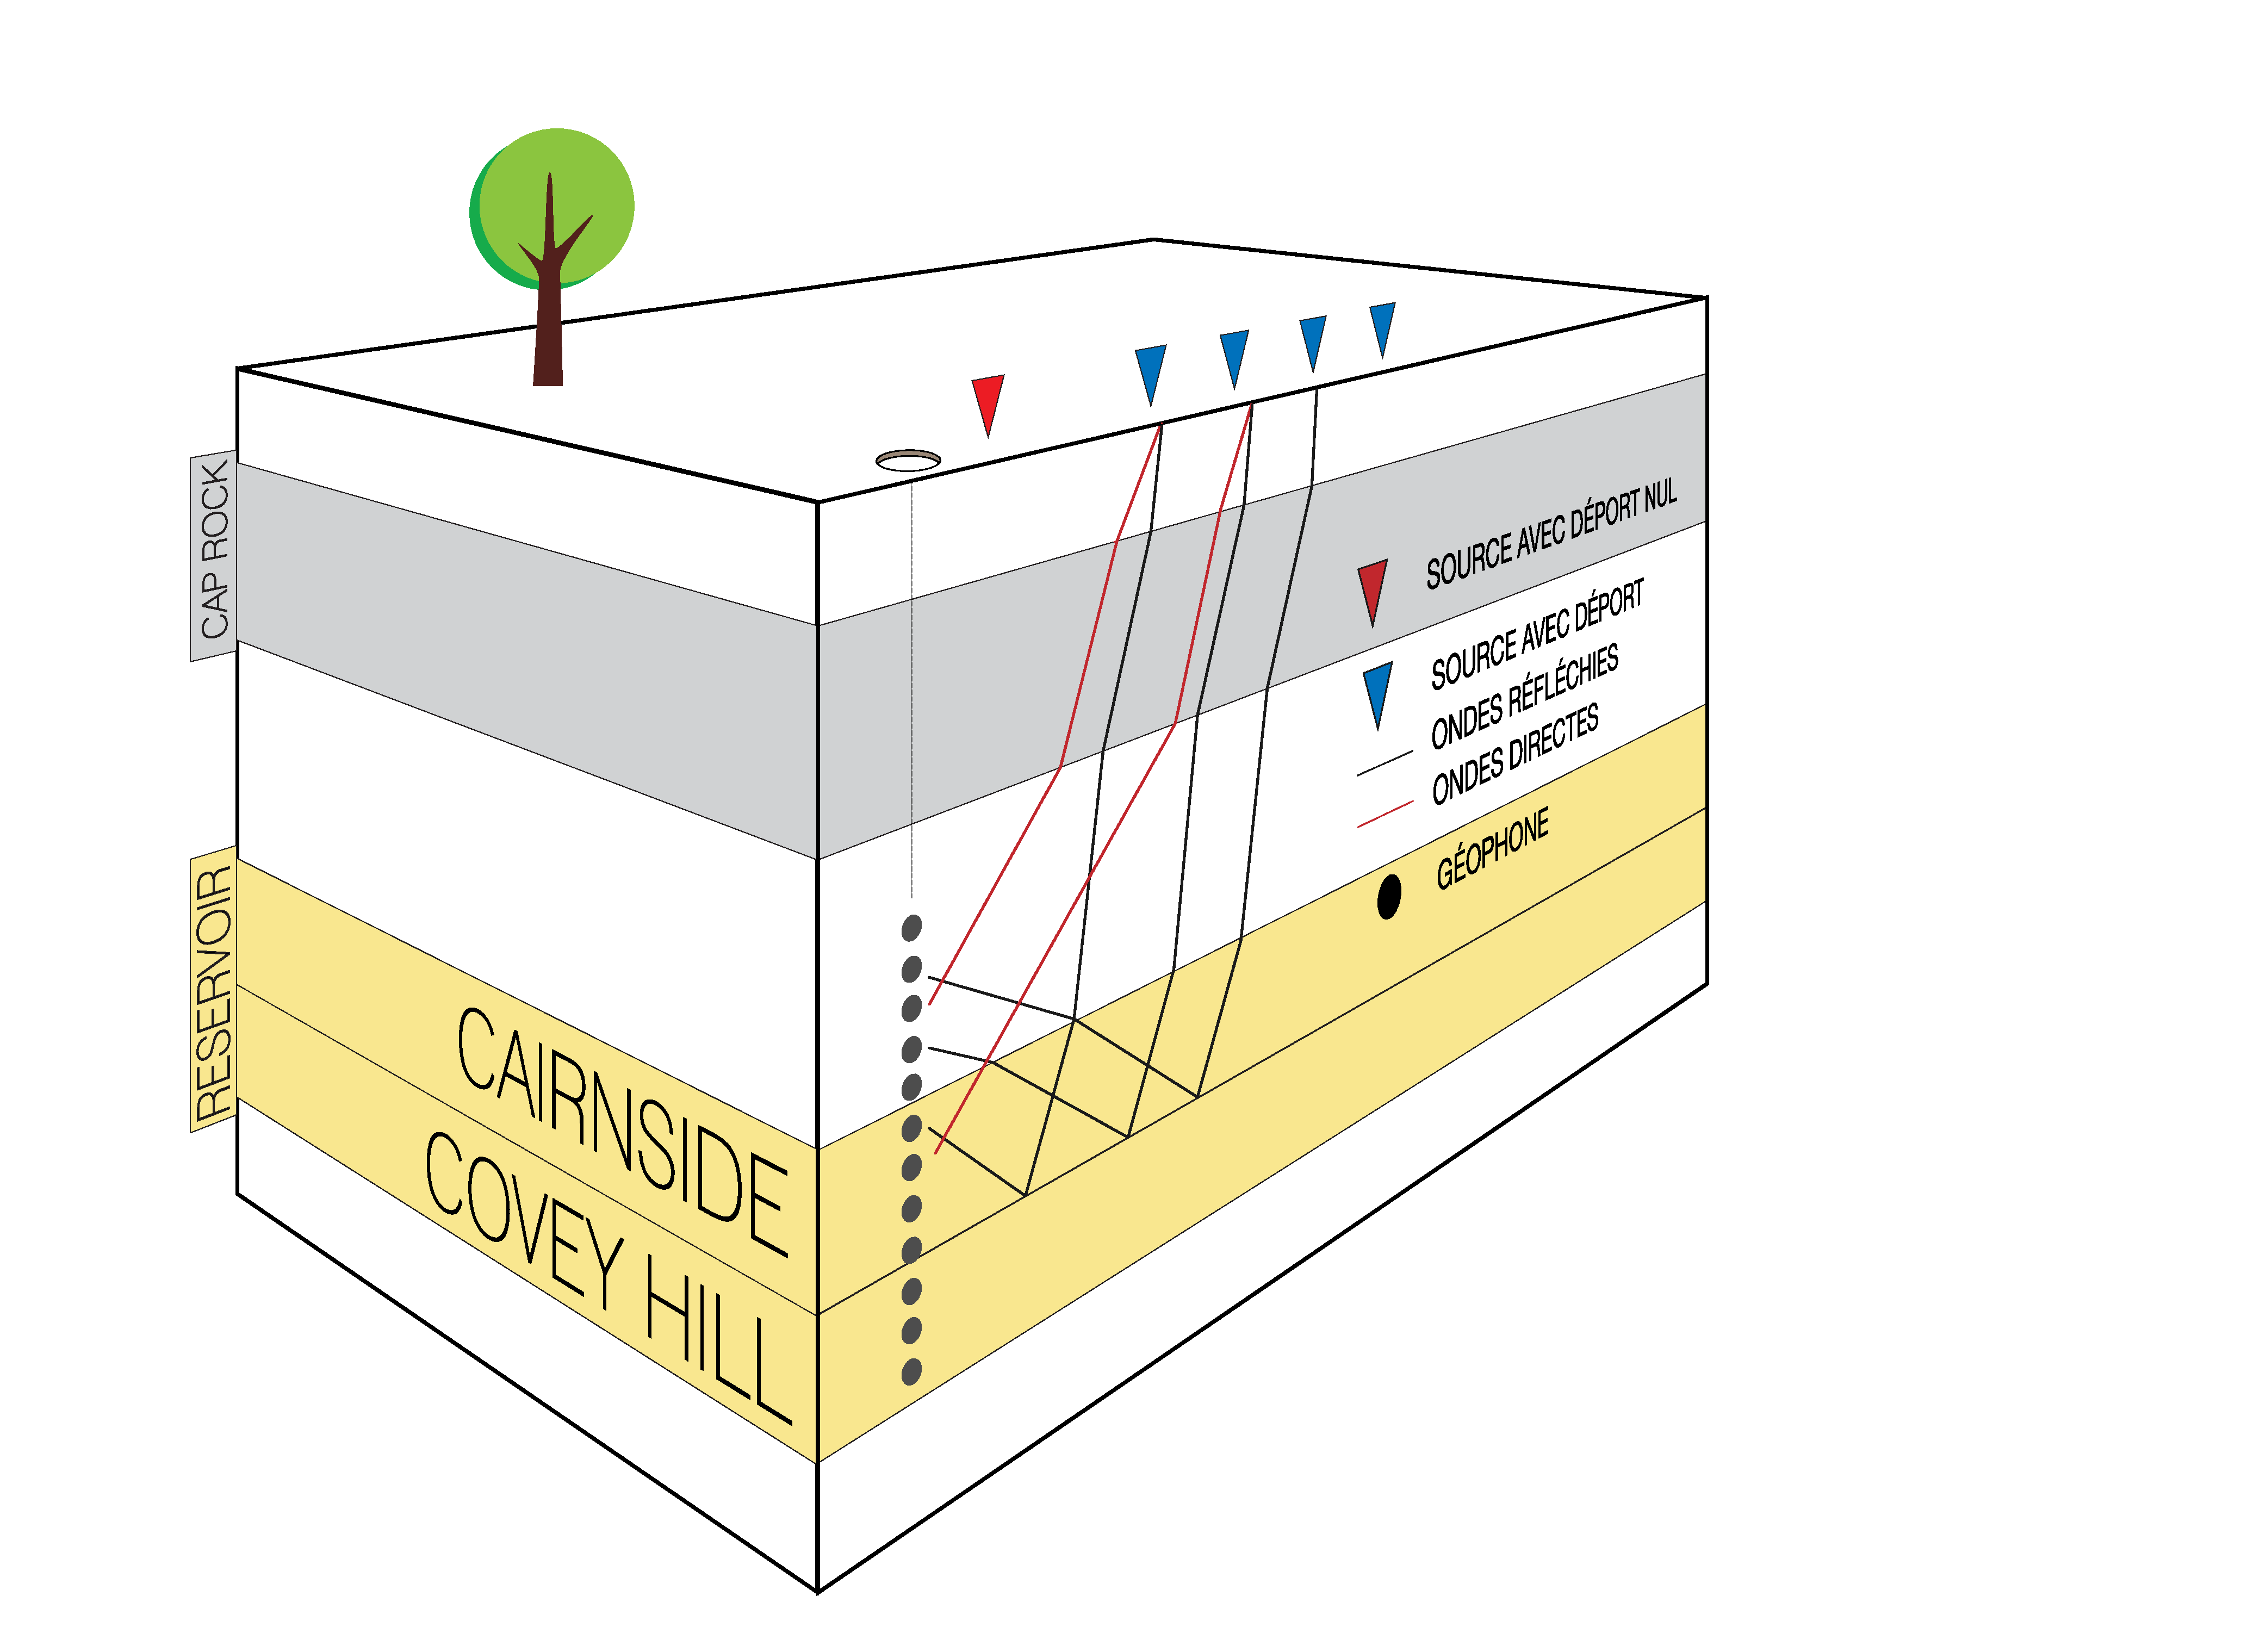
\includegraphics[width=0.8\textwidth]{fig/vsp_3D.pdf}
\caption{Schéma de la géométrie d'acquisition PSV}
\label{fig:vsp_3D}
\end{figure}
La \cref{fig:vsp_3D} montre le schéma d'une acquisition PSV. Une revue
exhaustive de cette méthode est présentée dans \citep{Hardage1992,Mari2003}
\subsection{Modèle géologique}
Le modèle géologique utilisé pour la modélisation sismique a été généré à partir
de données acquises dans plusieurs forages disponibles dans la zone d'étude
\citep{Claprood2012,TranNgoc2014}. À partir des diagraphies, un forage
synthétique représentatif pour la région d'étude a été construit pour les valeurs de $V_p$,
$V_s$, densité et porosité (voir \cref{fig:well-log} de l'article II à la
\cpageref{fig:well-log}). Pour chaque formation, les distributions de $V_p$,
$V_s$, densité et porosité ont été calculées, ainsi que leurs variogrammes
verticaux. À partir de ces distributions, un modèle de référence a été généré en
utilisant une approche par cosimulation séquentielle gaussienne,
méthode couramment utilisée pour la modélisation des propriétés géologiques à
partir de données de forages \citep{Deutsch1998,Doyen2007}. Le modèle pour les vitesses
des ondes $P$ est présenté à la \cref{fig:mod_ref_vp}.
\begin{figure}[ht]
\centering
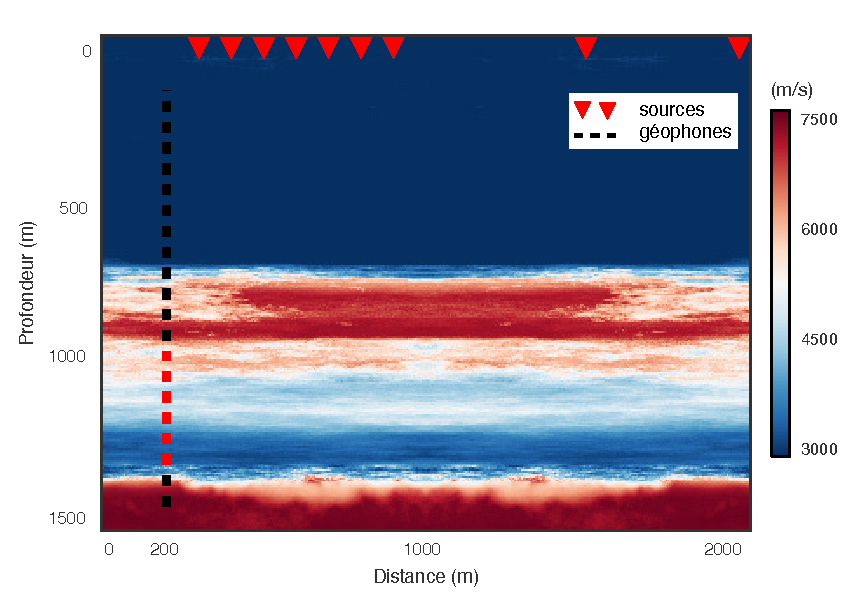
\includegraphics[width=0.8\textwidth]{fig/mod_ref_vp.pdf}
\caption{Modèle de référence pour $V_p$}
\label{fig:mod_ref_vp}
\end{figure}
Le modèle, qui fait \SI{2000 x 1500}{\metre} avec un pas de \SI{1 x
1}{\metre} pour un total de \num{3} millions de nœuds, est présenté à la
\cref{fig:mod_ref_vp}. Le \cref{tbl:modele} résume les caractéristiques
physiques du modèle.
\subsection{Modélisation sismique}
\label{sc:poroviscoelastique}
Un code poroviscoélastique basé sur les travaux de
\citet{Carcione1995,Carcione1996,Carcione1999} et implémenté par
\citet{Giroux2012} a été utilisé pour générer des sismogrammes synthétiques.
L'objectif était d'étudier la performance du PSV pour détecter les changements
sur le signal sismique dus à l'injection du \ce{CO2}. Cette formulation prend en
compte 12 paramètres, à savoir le module de la roche sèche ($K_{dry}$), le
module des minéraux de la roche ($K_s$), le module des fluides interstitiels
($K_{f}$), la porosité ($\phi$), le module de cisaillement de la roche ($G_s$),
la densité des minéraux de la roche ($\rho_s$), la densité des fluides
interstitiels ($\rho_f$), la tortuosité ($\tau$), la viscosité des fluides
($\eta$), la perméabilité ($\kappa$) et le facteur de qualité ($Q$). Le
\cref{tbl:modelpar} de l'article I à la \cpageref{tbl:modelpar}, résume les 12
paramètres du modèle géologique utilisé pour la modélisation sismique. \\
La \cref{fig:mod_ref_vp} montre la géométrie d'acquisition choisie pour la
modélisation. Les sources sont placées à la surface du modèle avec un déport
allant de \SIrange{100}{2000}{\metre} avec un espacement de \SI{100}{\metre}
pour le premier \num{7} déports.
Les géophones sont déployés sur une profondeur allant de \SIrange{200}{1400}{\metre} avec un espacement de
\SI{5}{\metre}. Sur la \cref{fig:mod_ref_vp}, les géophones qui se trouvent dans
le réservoir (Formation du Covey Hill et Cairnside) sont mis en évidence en
rouge.
L'objectif de la modélisation sismique est de simuler des acquisitions PSV
effectuées \numlist{5;15;50} ans après
injection de \ce{CO2}.
\begin{table}
  \centering
  \caption{Caractéristiques du modèle géologique et géométrie d’acquisition
PSV.}
 \begin{tabular}{p{5cm}c}
\toprule
 {Paramètre}  & {Valeur}   \\
\midrule
% Avg. porosity &(\si{\percent})  &  9.75  &  20   \\
% Avg. permeability & (\si{\metre\squared})  & 3.06e-16  & 6.5e-13  \\
Portée en x  & \SI{2000}{\metre}   \\
Portée en z  & \SI{1500}{\metre}   \\
Nœuds  & \num{3} millions   \\
% Injection depth &(\si{\metre}) & \multicolumn{2}{c}{1200-1350 }  \\
% Injection rate &(\si{\tonne\per\metre}) & \multicolumn{2}{c}{45 }  \\
% Injection time &(years) & \multicolumn{2}{c}{15 }  \\
% Migration time &(years) & \multicolumn{2}{c}{35}  \\
% Total storage &(\si{\kilo\tonne}) & \multicolumn{2}{c}{245}\\
Déport des sources  & \SIrange{100}{700}{\metre}    \\
Espacement des sources  & 1\SI{100}{\metre} \\
Coordonnée x des géophones  & \SI{200}{\metre} \\
Coordonnée z des géophones  & \SIrange{200}{1400}{\metre} \\
Espacement des géophones  & \SI{5}{\metre} \\
Traces totales  & 241 \\
\bottomrule
\end{tabular}
\label{tbl:modele}
\end{table}
\subsubsection{Séquence de traitement}
La séquence de traitement s'inspire du travail de
\citet{Coulombe1996,Zhang2010}. Le \cref{tbl:process} de l'article I à la
\cpageref{tbl:process} et la \cref{fig:traitement} résument les étapes du
traitement. Il s'agit d'un traitement classique pour les données de PSV, il ne
sera pas donc détaillé ici. La séquence de traitement a été appliquée uniquement
au déport inférieur à \SI{700}{\metre}; en effet pour les plus grands déports
(\SIlist{1300;1800} ), une onde réfractée apparaît à l'interface entre la
Formation du Lorraine-Utica et le Groupe Trenton, comme le montre la
\cref{fig:refracted} de l'article I à la \cpageref{fig:refracted} et qui empêche
la séparation des ondes montantes et descendantes et donc le traitement du PSV.
L'analyse des variations des amplitudes avec déports (\emph{Amplitude variation
with offset - AVO}) a été donc limitée aux déports inférieurs à
\SI{700}{\metre}.
\begin{figure}[!ht]
\centering
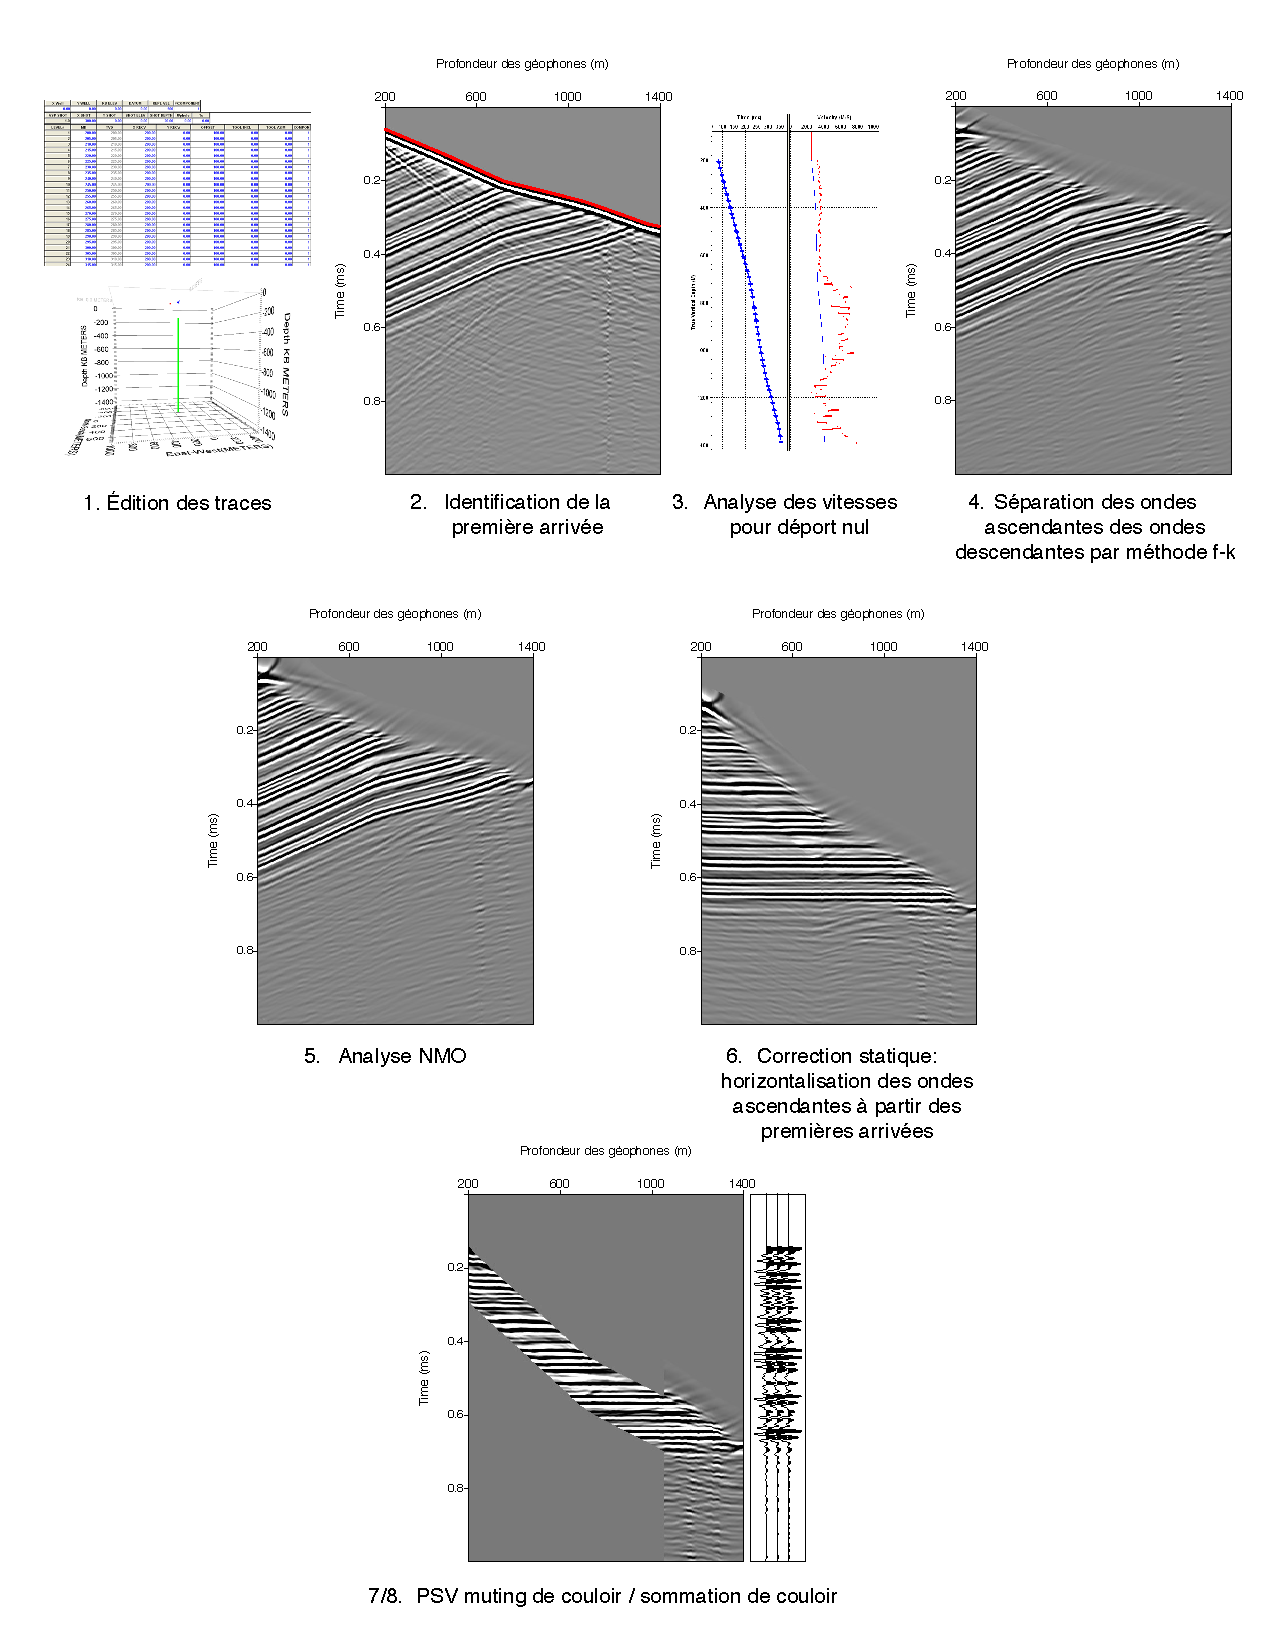
\includegraphics[width=1\textwidth]{fig/traitement.pdf}
\caption{Illustration de la séquence du traitement pour le Profilage Sismique
Verticale (PSV).}
\label{fig:traitement}
\end{figure}
\subsection{Modélisation de l'écoulement du \texorpdfstring{\ce{CO2}}{CO2}}
\label{sc:ecouelement}
Les approches classiques pour la modélisation de l'injection du \ce{CO2}
utilisent
des méthodes numériques en trois dimensions afin de reproduire avec un degré
élevé de précision les effets de l'hétérogénéité et de la dispersion
\citep{White1997,Pruess1999,Pruess2004,Schlumberger2007}. Cependant, ces
méthodes requièrent des efforts de calculs notables.\\
En partant d'hypothèses simplificatrices, des modèles qui demandent beaucoup moins
d'effort de calcul peuvent être développés. Une de ces hypothèses est d'utiliser
des méthodes semi-analytiques. Ce sont ces méthodes qui ont été les plus développées ces
dernières années
\citep{Nordbotten2004,Nordbotten2005a,Nordbotten2005,Nordbotten2009}. Cette
méthode suppose que l’aquifère est homogène et horizontal, qu'il y a une
interface définie entre les deux fluides (\ce{CO2} injectée et saumure) et que
la géométrie d'injection du \ce{CO2} est à symétrie radiale \citep{Gasda2009}.
Avec ces contraintes, les méthodes analytiques deviennent un outil puissant pour
la modélisation de l'injection et de la migration du \ce{CO2}.\\
Une méthode prometteuse pour la modélisation rapide et précise de la
séquestration du \ce{CO2} est basée sur l'hypothèse de l'équilibre vertical
(VE). Les modèles formulés par VE ont une longue tradition pour la simulation
des processus d'écoulement dans les milieux poreux; en hydrogéologie ils sont
connus comme approximation de Dupuit, tandis que dans l'industrie pétrolière ils
sont utilisés pour la simulation de l’écoulement multiphase
\citep{Martin1958,Coats1967,Martin1968}.\\
Pour modéliser l'écoulement après \numlist{5;15;50} ans du début de l'injection,
le modèle à équilibre vertical développé par \citet{Ligaarden2010} et contenu
dans MRST - \emph{Matlab Reservoir Simulation Toolbox} \citep{Lie2012} a été
utilisé. Dans cette formulation, la saturation moyenne est $s=\frac{h}{H}$ et
correspond à la hauteur relative du panache de \ce{CO2}, comme montré sur la
\cref{fig:VE}.
\begin{figure}[!ht]
\centering
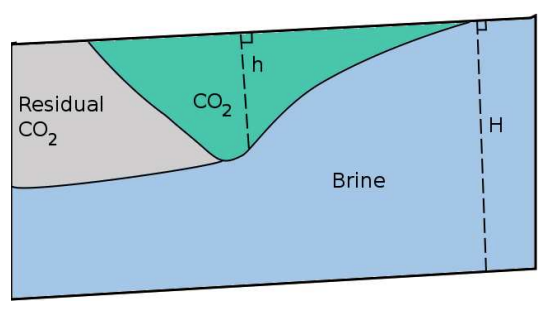
\includegraphics[width=0.7\textwidth]{fig/VE.png}
\caption{Illustration du panache de \ce{CO2} assumé dans les modèles à équilibre
vertical (VE), d'après \citet{Ligaarden2010}.}
\label{fig:VE}
\end{figure}
La \cref{fig:res} montre les distributions de porosité et de perméabilité au
niveau du réservoir (Formation du Cairnside et du Covey Hill), qui sont utilisées
pour simuler l'injection du \ce{CO2}. La pérméabilité est dérivée en utilisant
une extension de l'équation de Kozeny-Carman \citep{Kozeny1927,Carman1938}:
\begin{equation}
k = \dfrac{1}{72}\dfrac{\phi^3}{(1-\phi)^2\tau^2}d^2,
\end{equation}
où $d$ est le diamètre des grains qui composent la roche et $\tau$ la tortuosité. Pour des grès très
compacts, $k$ est de l'ordre \SI{5e-6}{\metre}
\citep{DonaldRWiesnet1961}.
\begin{figure}[!ht]
        \centering
        \begin{subfigure}[b]{1\textwidth}
                \caption{Porosité}
                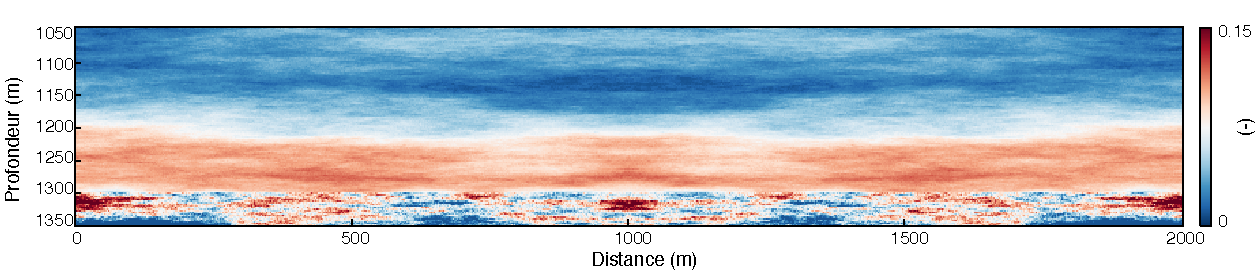
\includegraphics[width=\textwidth]{fig/phi_res.pdf}
                \label{fig:phi_res}
        \end{subfigure}%

        \begin{subfigure}[b]{1\textwidth}
                \caption{Perméabilité}
                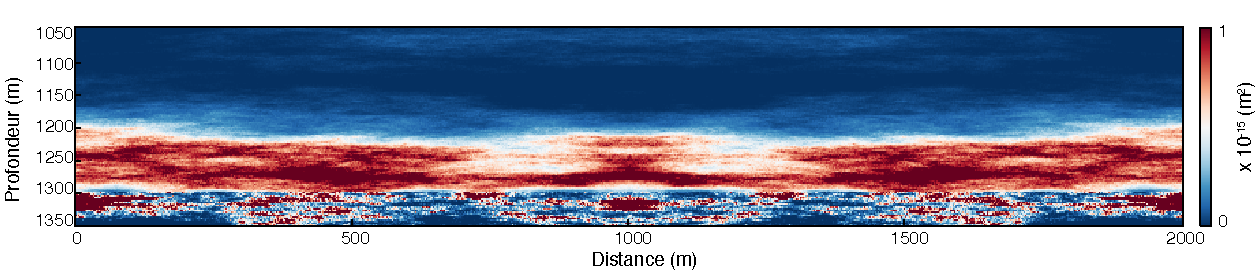
\includegraphics[width=\textwidth]{fig/K_res.pdf}
                \label{fig:K_res}
        \end{subfigure}

        \caption{Distribution de la porosité et de la perméabilité dans le
réservoir.}
        \label{fig:res}.
\end{figure}
La simulation de l'écoulement se fait dans la formation du Covey Hill
(\SIrange{1200}{1350}{\metre}). Les \cref{fig:5r,fig:15r,,fig:50r} montrent
l'extension et la saturation du panache de \ce{CO2} après \numlist{5;15;50}
ans.\par

Un deuxième scénario, avec une porosité moyenne de \SI{20}{\percent} dans le
réservoir (scénario optimal) a été étudié. Les résultats des simulations
d'écoulement de \ce{CO2} sont présentés aux \cref{fig:5o,fig:15o,,fig:50o}. Pour
ce scénario, l'extension du panache est logiquement plus grande. Les paramètres
principaux pour les deux scénarios sont résumés dans le \cref{tbl:co2par} de
l'article I à la \cpageref{tbl:co2par}.
% \begin{landscape}
\begin{figure}[p]
        \centering
        \begin{subfigure}[b]{.47\textwidth}
                \caption{5 ans après injection \\ Scénario réaliste }
                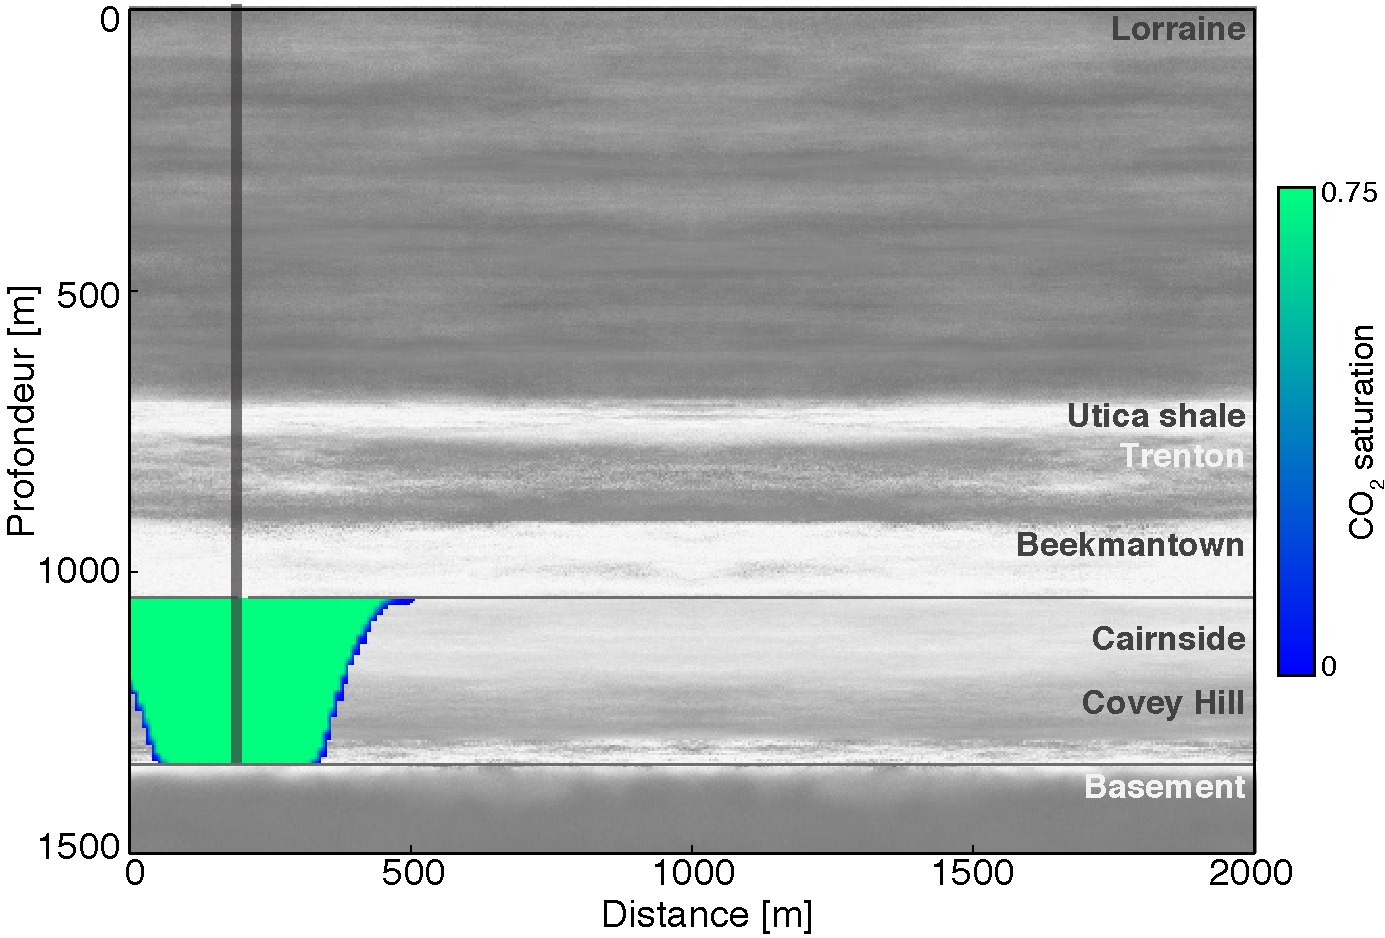
\includegraphics[width=\textwidth]{fig/5r.pdf}
                \label{fig:5r}
        \end{subfigure}
        \qquad
        \begin{subfigure}[b]{.47\textwidth}
                \caption{5 ans après injection \\ Scénario optimal}
                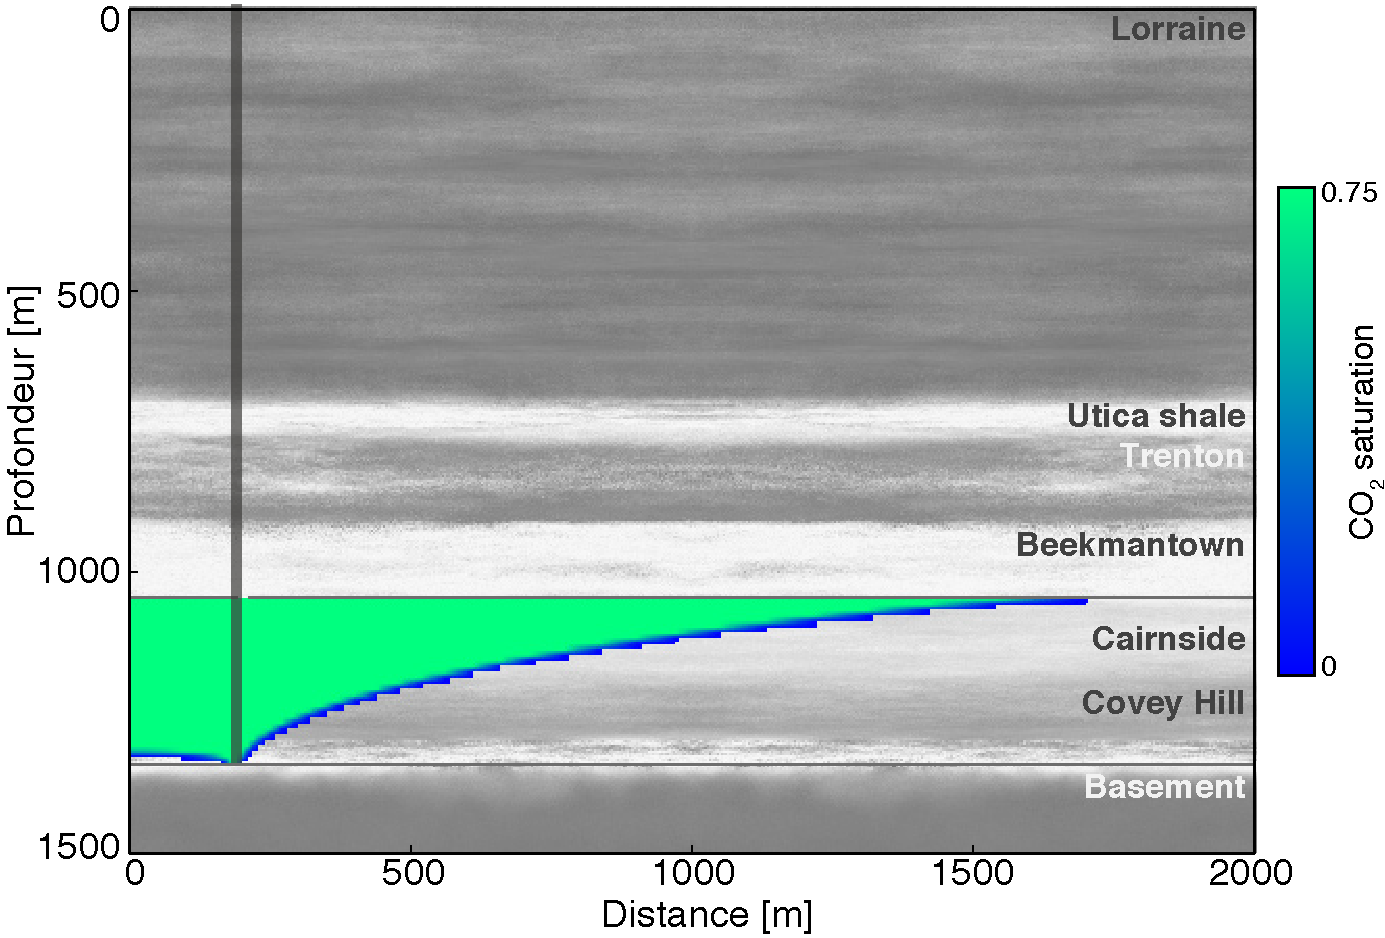
\includegraphics[width=\textwidth]{fig/5o.pdf}
                \label{fig:5o}
        \end{subfigure}

        \begin{subfigure}[b]{.47\textwidth}
                \caption{15 ans après injection }
                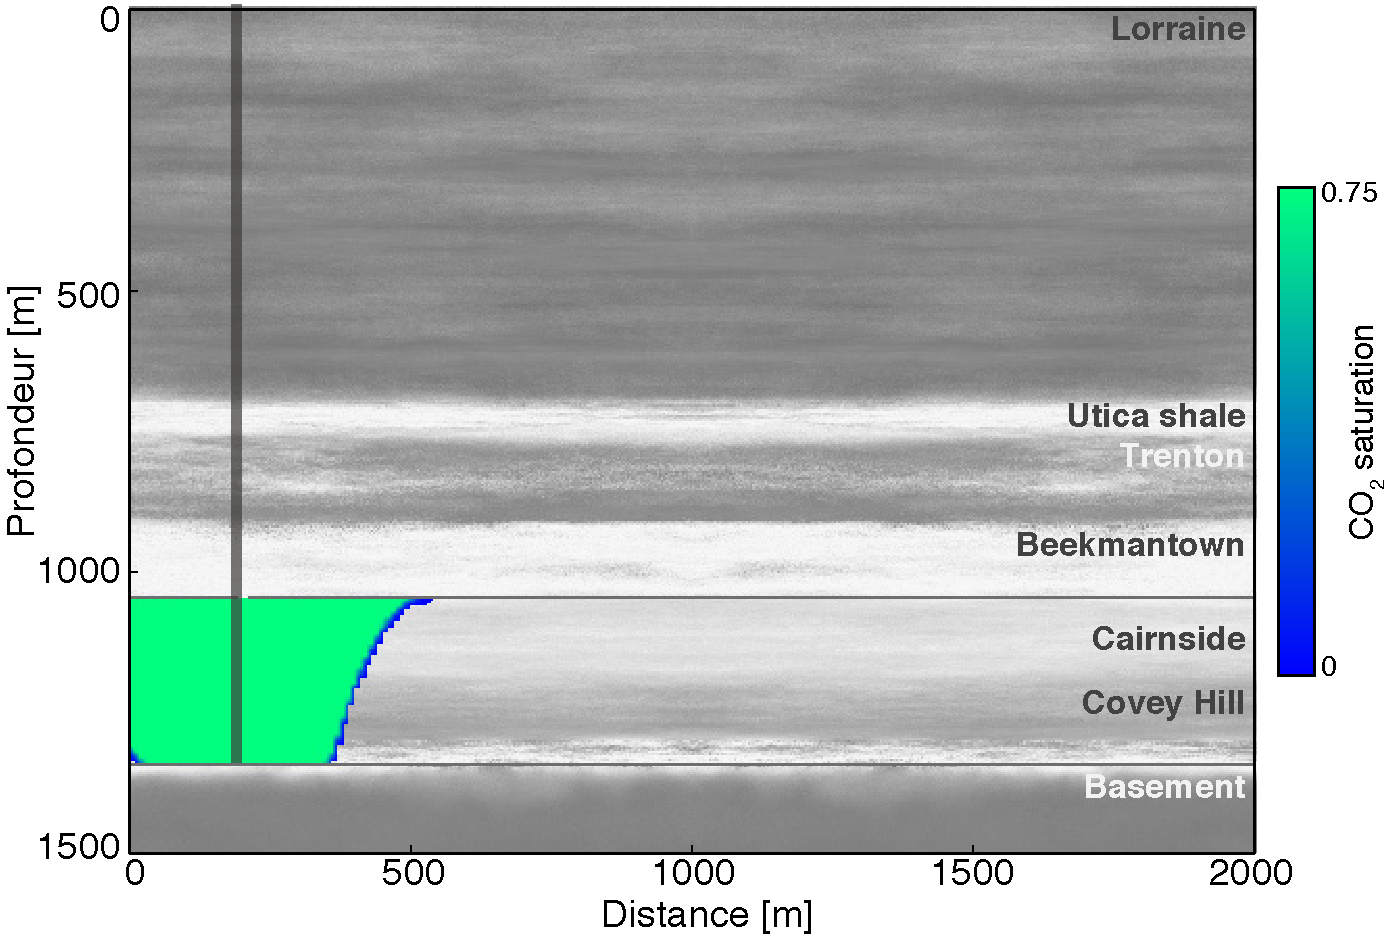
\includegraphics[width=\textwidth]{fig/15r.pdf}
                \label{fig:15r}
        \end{subfigure}
        \qquad
        \begin{subfigure}[b]{.47\textwidth}
                \caption{15 ans après injection  }
                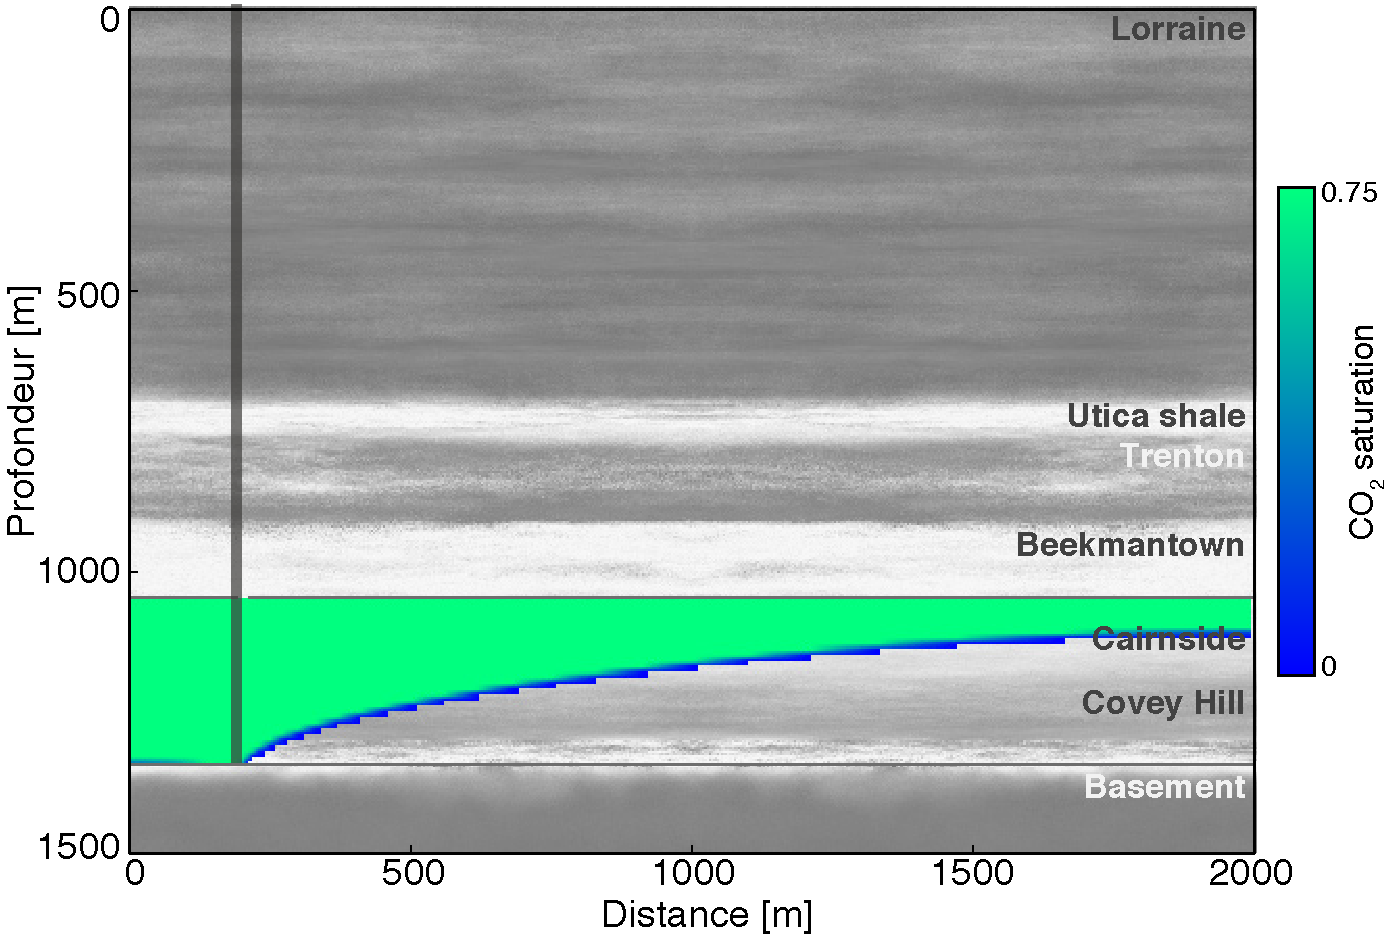
\includegraphics[width=\textwidth]{fig/15o.pdf}
                \label{fig:15o}
        \end{subfigure}

        \begin{subfigure}[b]{.47\textwidth}
                \caption{50 ans après injection }
                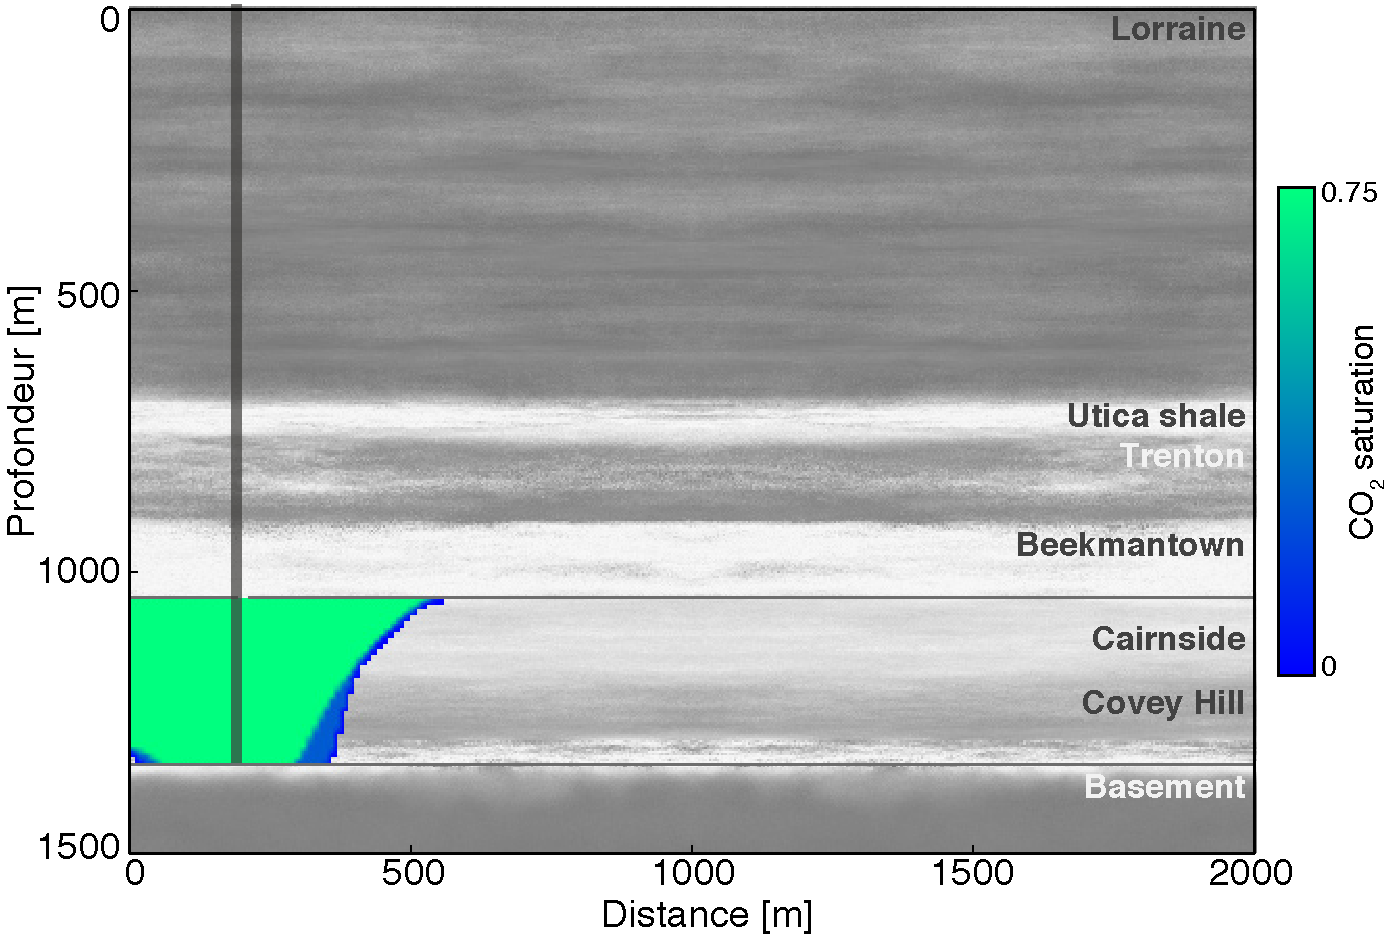
\includegraphics[width=\textwidth]{fig/50r.pdf}
                \label{fig:50r}
        \end{subfigure}
        \qquad
         \begin{subfigure}[b]{.47\textwidth}
                \caption{50 ans après injection}
                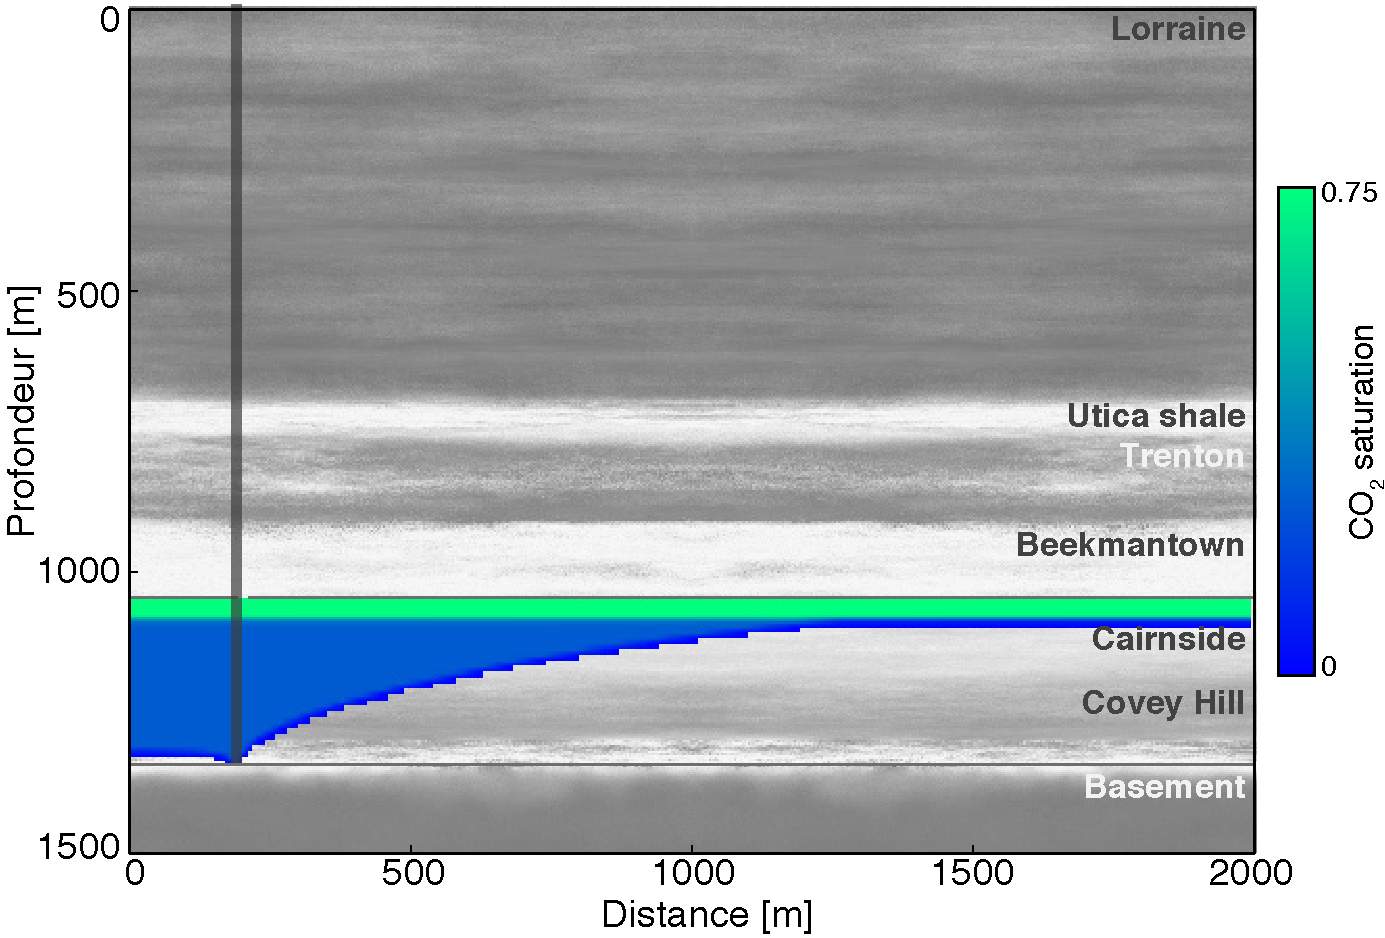
\includegraphics[width=\textwidth]{fig/50o.pdf}
                \label{fig:50o}
        \end{subfigure}

        \caption{Saturation du panache du \ce{CO2} en fonction du temps.}
        \label{fig:co2_sat}.
\end{figure}
% \end{landscape}
\subsection{Synthèse des résultats}
Cette section présente une synthèse des résultats obtenus, qui sont discutés plus
en détail dans l'article I.
Les \cref{fig:seism_opt_a,fig:seism_opt_b,fig:seism_opt_c,fig:seism_bec_a,fig:seism_bec_b,fig:seism_bec_c}
de l'article I aux \cpageref{fig:seismopt,fig:seismbec} montrent les résultats
pour les suivis à \numlist{5;15;50} ans des scenarii, respectivement optimal et réaliste. Les deux figures montrent la sommation des traces pour les
déports allant de \SIrange{100}{700}{\metre}.
Pour chaque suivi, la comparaison avec le suivi précédent ainsi que leur
différence sont montrés.\\
Pour les deux scénarios, un délai dû à l'injection du \ce{CO2} est détecté à
partir de \SI{550}{\milli\second}. Ce delai est de l'ordre de
\SI{30}{\milli\second} à la base du réservoir
(\cref{fig:seism_opt_a,fig:seism_bec_a}), comme décrit dans le \cref{tbl:delay}
de l'article I à la \cpageref{tbl:delay}. Le suivi à \num{15} ans pour le
scénario optimal ne montre aucune différence avec le suivi à \num{5} ans
\cref{fig:seism_opt_b}. Pour la période de migration du \ce{CO2}
(\numrange{15}{50} ans), il y a dissolution partielle du \ce{CO2}. Ce phénomène
est plus accentué dans le scénario optimal et il se reflète dans les traces
sommées, avec une arrivée anticipée pour le
réflecteur à \SI{700}{\milli\second} comparé au même réflecteur pour le suivi à
\num{15} ans (\cref{fig:seism_opt_c,fig:seism_bec_c}. Pour le scénario réaliste, on
peut observer une anomalie AVO à la base du réservoir. \\
Une comparaison entre le modèle hétérogène proposé et un modèle homogène
stratifié classique a été effectuée et les résultats sont présentés avec les
\cref{fig:stochvsblock_a,fig:stochvsblock_a} de l'article I à la
\cpageref{fig:stochvsblock_a} pour un suivi après \num{5} ans du début de
l’injection, pour le scénario réaliste. Cette comparaison permet d’évaluer les
différentes réponses sismiques produites par les deux modèles. Par exemple, le
réflecteur à \SI{700}{\milli\second} montre une diminution de l'amplitude avec
l'augmentation du déport pour le modèle homogène classique, tandis que pour le
modèle hétérogène le même réflecteur montre une augmentation de l'amplitude avec
le déport. Ce phénomène est confirmé avec l’analyse de Zoeprritz \citep{Aki1980}
dans la \cref{fig:zoeppritz} de l'article I à la \cpageref{fig:zoeppritz}.

%!TeX root = Thesis_LP.tex
\chapter{La géostatistique comme outil d’optimisation}
\label{sc:geostat}
Cette section résume brièvement les aspects théoriques et les démarches
méthodologiques effectuées pour répondre à l'objectif formulé dans la
\cref{sc:obj2}. La \cref{sc:inversion_optimisation} présente les concepts de
base de l'inversion stochastique et des méthodes d'optimisation. La
\cref{sc:application} décrit l'application de la méthodologie développée à un
exemple synthétique. Les détails précis de la méthodologie utilisée se
retrouvent dans l’article II faisant partie de cette thèse.
\section{Inversion stochastique}
\label{sc:inversion_optimisation}
Les données géophysiques sont couramment utilisées dans la caractérisation de
réservoir, pas seulement pour obtenir une description géométrique des structures
géologiques, mais aussi pour en estimer les propriétés physiques.
La transformation de données géophysiques en propriétés physiques telles que les
paramètres élastiques ou électriques peut être posée comme un problème inverse
non unique \citep{Bosch2010}. Tout problème d'inversion peut être posé comme un
problème d'inférence bayésienne, c'est-à-dire mettre à jour la connaissance au
préalable représentée par des observations
\citep{Tarantola2004,Duijndam1988b,Duijndam1988,Ulrych2001}. Les solutions d'un
problème inverse sont un ensemble de modèles géologiques qui s'ajustent, en
terme de modélisation directe et avec une certaine tolérance, aux données
réelles. En sismique, les inversions permettent d'obtenir des propriétés
élastiques telles que l’impédance acoustique, la vitesse des ondes $P$ et $S$
ainsi que la densité. Pour la caractérisation de réservoir, ces propriétés
élastiques doivent être transformées en propriétés de réservoirs telles que
porosité, lithologie et saturation, en utilisant des modèles pétrophysiques
\citep{Bosch2010}.\\
Il existe plusieurs méthodologies qui combinent l'inversion sismique, la
géostatistique, et les modèles pétrophysiques pour prédire les propriétés des
réservoirs. Ces méthodologies peuvent être regroupées en 2 catégories: les
méthodes par approche séquentielle \citep{Dubrule2003,Doyen2007} où les données
sismiques sont inversées pour obtenir les propriétés élastiques et ensuite les
propriétés de réservoir sont classifiées en utilisant des techniques
statistiques comme, par exemple, la classification bayésienne; et les méthodes
par
inversions stochastique qui tentent d'inférer directement les propriétés
géologiques à partir
des données sismiques et de puits. \citep{Grana2012}.\\
Les approches par inversion stochastique sont généralement basées sur
l'application itérative d'un modèle direct et l'étape d'inversion est effectuée
en utilisant des techniques déterministes ou stochastiques. En particulier, des
modèles de propriétés géologiques sont générés à partir des données de puits;
des transformations
pétrophysiques sont ensuite appliquées de façon à générer les volumes
correspondants des propriétés élastiques. Finalement, des sismogrammes
synthétiques sont calculés et sont comparés  aux données sismiques réelles afin
d'évaluer les écarts. Les modèles initiaux sont générés en utilisant des
méthodes géostatistiques telles que la cosimulation séquentielle gaussienne
\citep{Deutsch1998,Doyen2007}. Le modèle final est trouvé en appliquant une
méthode d’optimisation appropriée. Le flux de travail d’inversion stochastique
classique est montré à la \cref{fig:inversion}. Différentes méthodes
d'optimisation peuvent être utilisées. Des approches d'optimisation stochastique
basée sur les méthodes Monte-Carlo ont été proposées par différents auteurs
\citep{Eidsvik2004,Larsen2006,Gunning2007,Rimstad2010,Ulvmoen2010,Hansen2012}.
\citet{Grana2012} a montré l’efficacité de la méthode basée sur la perturbation
probabiliste \citep{Caers2006} pour estimer des modèles de réservoirs.
\citet{Bosch2010} présente une revue des méthodes d'optimisation.
\begin{figure}[!ht]
\centering
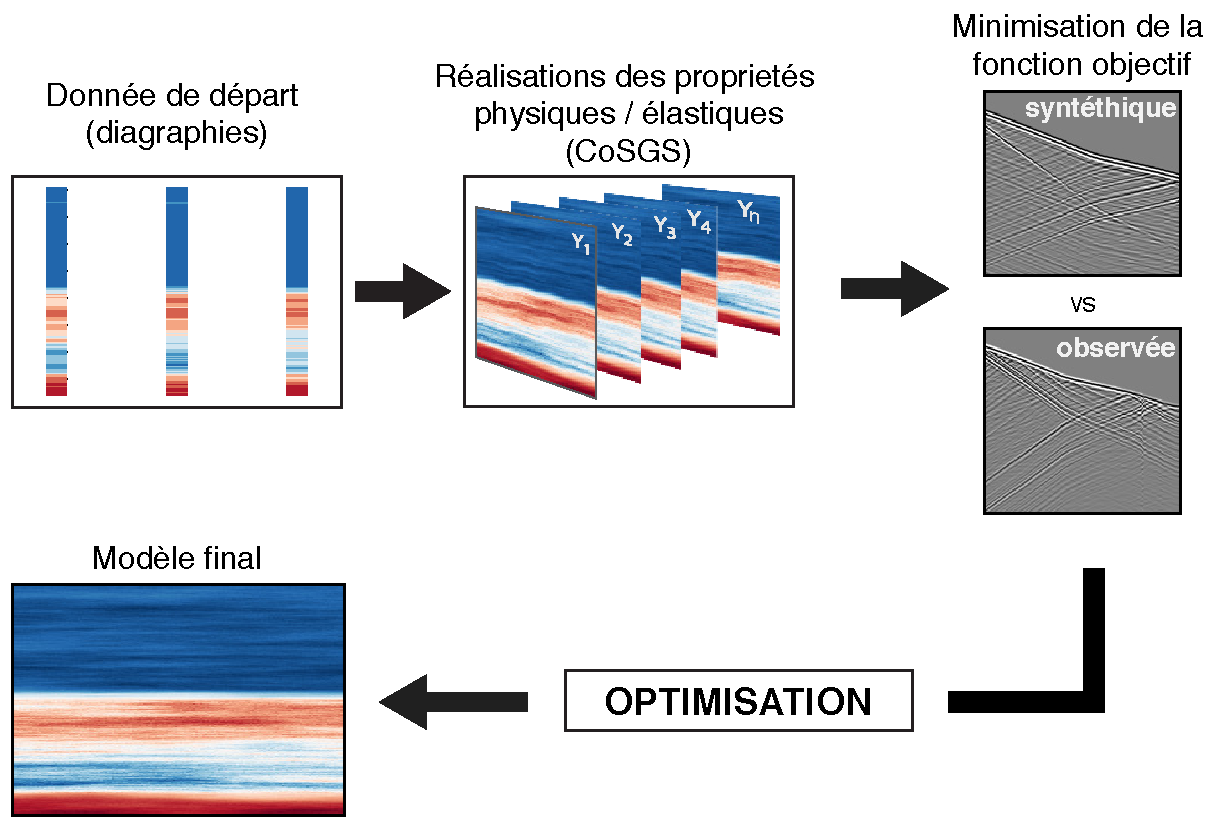
\includegraphics[width=1\textwidth]{fig/inversion.pdf}
\caption{Flux de travail classique de l'inversion stochastique}
\label{fig:inversion}
\end{figure}
\subsection{La déformation graduelle comme méthode d'optimisation}
La méthode de déformation graduelle est une technique pour générer des modèles
stochastiques qui sont graduellement déformés, mais qui préservent leur
continuité spatiale. Cette technique a été développée initialement par
\citet{Hu2000} afin de déformer des champs aléatoires gaussiens. À partir de
deux réalisations gaussiennes indépendantes $Y_1$ et $Y_2$ de moyenne nulle et
covariance spatiale identique, une nouvelle réalisation est définie en combinant
$Y_1$ et $Y_2$ selon la relation suivante:
\begin{equation}
Y(t) = Y_1 \cos(t) + Y_2 \sin (t).
\label{eq:dg}
\end{equation}
La nouvelle réalisation $Y(t)$ a aussi une moyenne nulle et la même
covariance que $Y_1$ et $Y_2$. À partir de deux distributions indépendantes, on
obtient donc une chaîne de réalisations $Y(t)$ en faisant varier le paramètre
$t$. En utilisant les fonctions sinus et cosinus dans l'\cref{eq:dg}, la
paramétrisation est périodique avec une période de \num{2}$\pi$ où $Y(t)$ =
$Y_1$ quand $t$ = \num{0} et $Y(t)$ = $Y_2$ quand $t$ =  $\pi/2$. \\
La méthode de déformation graduelle, qui s'intègre facilement dans un processus
d'optimisation, vise à minimiser la fonction objectif en faisant varier le
coefficient de déformation $t$ selon un processus de recherche itérative comme
il est présenté dans la \cref{fig:dg_iter} \citep{LeRavalec2005}.
\begin{figure}[!ht]
\centering
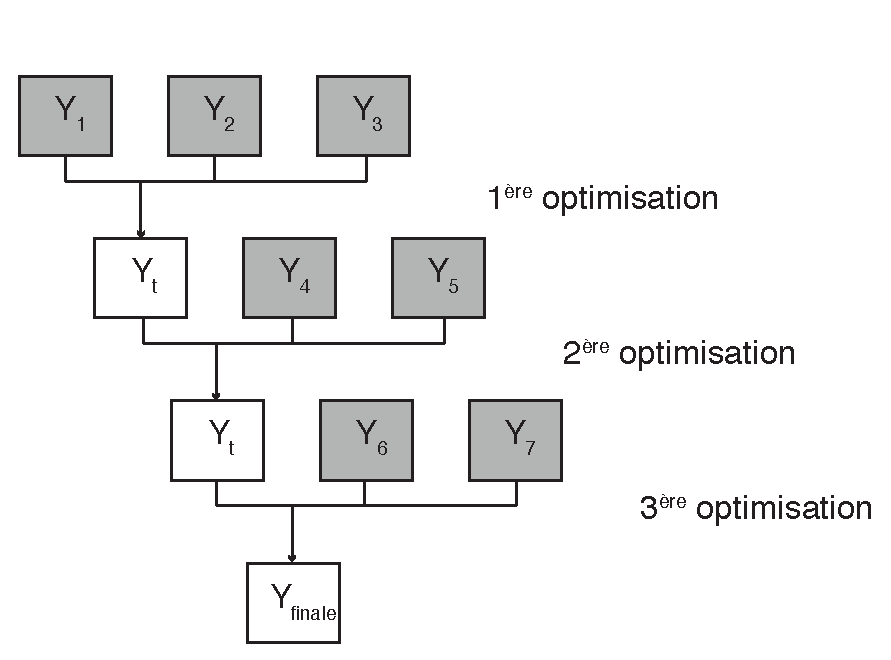
\includegraphics[width=0.7\textwidth]{fig/dg_iter.pdf}
\caption{Processus de recherche itérative impliquant la combinaison graduelle de
trois réalisations. D'après \citet{LeRavalec2005}.}
\label{fig:dg_iter}
\end{figure}
La \cref{sc:metho_art2} de l'article II à la page \cpageref{sc:metho_art2}
décrit en détail cette méthode.
\section{Application à un exemple synthétique}
\label{sc:application}
Le flux de travail d'optimisation a été appliqué à un modèle synthétique qui
représente un potentiel site pour le stockage du \ce{CO2} dans la région de
Bécancour, au Québec. La description du site est présentée à la
\cref{sc:site_etude} à la page \cpageref{sc:site_etude}. \\
La \Cref{fig:well-log} de l'article II à la page \cpageref{fig:well-log} montre
les diagraphies synthétiques pour les vitesses des ondes $P$ ($V_p$), la densité
($\rho$) et la porosité ($\phi$) pour les formations qui représentent la
séquence
sédimentaire des Basses-Terres du St Laurent, obtenues à partir de forages
disponibles dans la zone d'étude. Les vitesses des ondes $S$ ont été calculées
en utilisant la relation de Greenberg-Castagna \citep{Greenberg1992}.
La séquence sédimentaire a été divisée en 7 couches qui représentent les
formations principales de la séquence sédimentaire: Lorraine, Shale d'Utica,
Trenton, Beekmantown, Cairnside, Covey Hill et socle. Pour chaque groupe, les
distributions des diagraphies sont montrées tandis que les moyennes et les
écarts-types sont résumés dans le \cref{tab:well-log} de l'article II à la
\cpageref{tab:well-log}.\\
Le flux de
travail est divisé en trois étapes et il est montré à la \cref{fig:workflow} de
l'article II à la \cpageref{fig:workflow}: 1) générer des réalisations
stochastiques initiales à partir des diagraphies; 2) combiner les réalisations
dans une boucle d’optimisation statique; 3) combiner les modèles obtenus en 2)
dans une boucle d'optimisation dynamique.
\subsection{Modèle de référence}
Les distributions initiales de $V_p$, $V_s$, $\rho$ et $\phi$, sont utilisées
dans un algorithme de cosimulation séquentielle gaussienne  pour générer le
modèle de référence pour chaque paramètre. Le résultat du modèle de référence
pour $V_p$, $V_s$, $\rho$ et $\phi$ est montré à la \cref{fig:ref_model} de
l'article II à la page \cpageref{fig:ref_model}. L'algorithme est formulé de
manière à respecter la transition naturelle entre les différentes couches. \\
Le code poroviscoélastique développé par \citet{Giroux2012} et présenté dans la
\cref{sc:poroviscoelastique} du chapitre 2 est utilisé pour générer le
sismogramme synthétique de référence.
\subsection{Réalisations initiales}
La première étape du flux de travail consiste à générer des ensembles de 100
réalisations stochastiques par cosimulation séquentielle gaussienne.
L'algorithme de simulation séquentielle bayésienne est une méthode
géostatistique classique permettant de
générer
des réalisations des paramètres de réservoir tout préservant la covariance spatiale modélisée sur les données ainsi qu'ajuster parfaitement toutes les données. La continuité spatiale des réalisations est assurée par les modèles de
variogramme \citep{Doyen2007, Grana2012}.
\subsection{Optimisation statique}
Dans la deuxième étape, une première boucle d'optimisation basée sur la méthode
de déformation graduelle est appliquée à chaque ensemble de réalisations
initiales, comme il est montré à la \cref{fig:1boucle}.
\begin{figure}[!ht]
\centering
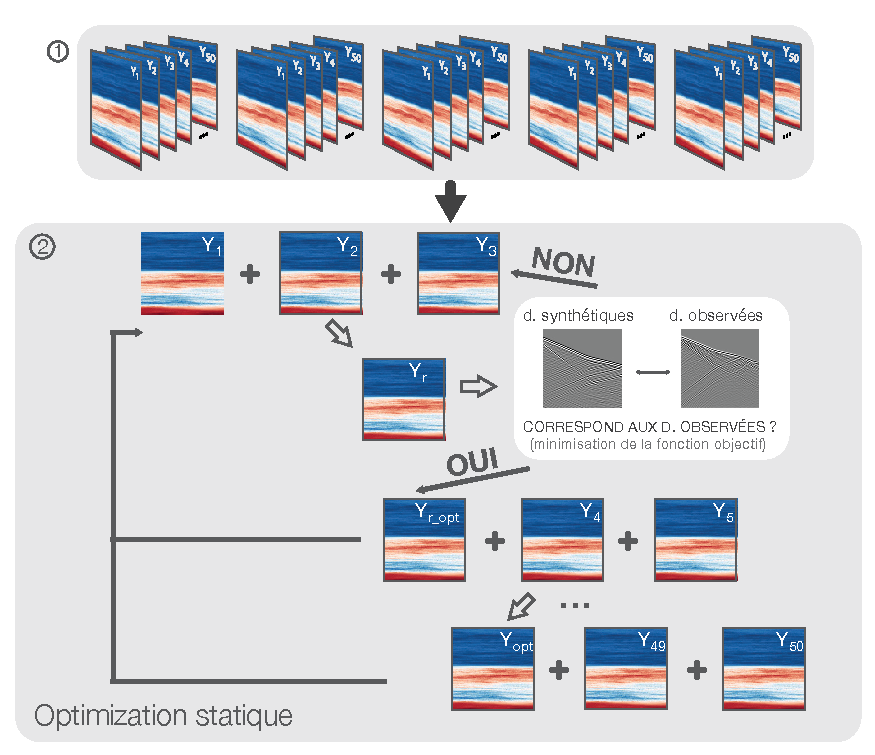
\includegraphics[width=0.7\textwidth]{fig/1boucle.pdf}
\caption{Boucle d'optimisation statique}
\label{fig:1boucle}
\end{figure}
L’optimisation est considérée statique, car uniquement basée sur les données de
forages. Pour chaque itération, trois réalisations sont combinées linéairement
et paramétrées selon la relation suivante:
\begin{equation}
\begin{cases}
    \alpha_1 = \dfrac{1}{3} + \dfrac{2}{3}\ cos(r),\\
    \alpha_2 = \dfrac{1}{3} + \dfrac{2}{3}\ sin\bigg(-\dfrac{\pi}{6}+r\bigg),\\
    \alpha_3 = \dfrac{1}{3} + \dfrac{2}{3}\ sin\bigg(-\dfrac{\pi}{6}-r\bigg).
    \end{cases}
\label{eq:eq_DG}
\end{equation}
Cette combinaison donne naissance à une nouvelle réalisation optimale au sens des données sismiques brutes mesurées, qui est ensuite
combinée avec \num{2} autres réalisations initiales et ainsi de suite jusqu'à ce
que toutes les réalisations initiales aient été combinées ensemble.
\subsubsection{Modélisation sismique directe}
À chaque itération, un sismogramme synthétique de l'onde complète pour les
déports proches, moyens et éloignés est modélisé en utilisant la formulation
viscoélastique  \citep{Bohlen2002} codée sur GPU (Graphics
Processing Unit) développé par \citet{Gab2014}. Ceci permet de tenir compte de
toutes les variations dans le signal sismique causé par l'injection du \ce{CO2}.
L'utilisation d'un GPU sur un poste de travail standard permet de réduire le
temps de la modélisation à chaque iteration de plus de 2 ordres de grandeur par
rapport à la version originale sur CPU en parallèle. Dans les faits, le temps
nécessaire pour modeliser la réponse sismique à chaque itération avec GPU est
d'environ \num{1} minute comparé à \num{25} minutes avec CPU.\\
Une fois que le sismogramme synthétique est calculé, il est comparé au sismogramme de référence afin de
minimiser les écarts entre observations et simulations. À la fin de la boucle,
on obtient la réalisation qui minimise ces écarts. Cette modélisation est considérée comme le "meilleur" modèle ajustant les données sismiques et de puits avant l'injection du \ce{CO2}.
\subsection{Optimisation dynamique}
Après l'optimisation statique, on obtient un modèle optimisé de $V_p$,
$V_s$, $\rho$ et $\phi$ pour chacun des 5 ensembles, qui sont combinés, par
déformation
graduelle, dans la boucle d'optimisation dynamique, comme il est montré à la
\cref{fig:2boucle}. À chaque itération, une simulation d'écoulement sur la
nouvelle réalisation est effectuée afin d'optimiser le modèle de réservoir en
fonction de l'injection et  de l'écoulement du \ce{CO2}. Comme pour la
précédente boucle, une modélisation sismique directe avec les nouvelles
propriétés élastiques est effectuée et le sismogramme synthétique est comparé au
sismogramme de référence afin de minimiser les écarts.
\begin{figure}[!ht]
\centering
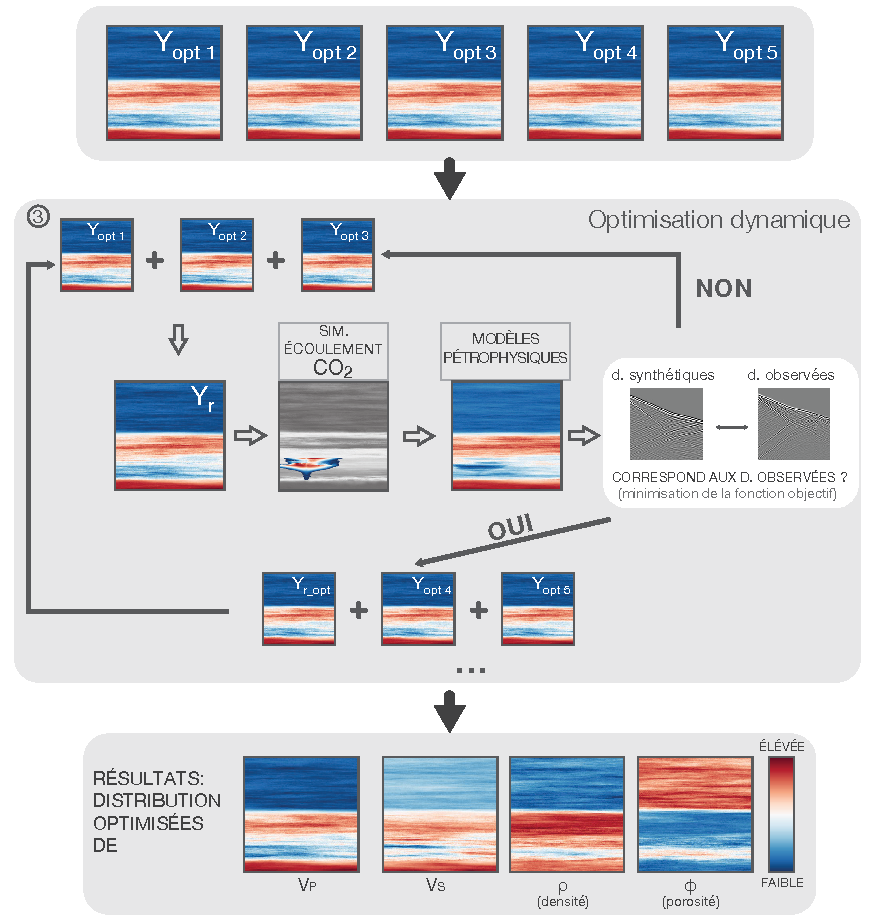
\includegraphics[width=0.7\textwidth]{fig/2boucle.pdf}
\caption{Boucle d'optimisation dynamique}
\label{fig:2boucle}
\end{figure}
À la fin de l'optimisation dynamique, on obtient le modèle de $V_p$, $V_s$,
$\rho$ et $\phi$ qui honore le modèle de référence à la fois pour les données
statiques et pour l'écoulement de \ce{CO2}. La \cref{fig:final_model} de
l'article II à la \cpageref{fig:final_model} montre le modèle final pour $V_p$,
$V_s$, $\rho$ et $\phi$.
\subsubsection{Simulation d'écoulement du \texorpdfstring{\ce{CO2}}{CO2}}
Au cours de ce projet de doctorat, le modèle à équilibre vertical développé par \citep{Ligaarden2010} et contenu
dans MRST - \emph{Matlab Reservoir Simulation Toolbox} \citep{Lie2012} a été
utilisé pour simuler l'injection de \ce{CO2} pendant \num{200} jours. Ce modèle
a été décrit dans la \cref{sc:ecouelement} du chapitre 2. Les résultats
de la simulation d'écoulement pour le modèle de référence, une réalisation
 initiale choisie au hasard ainsi que pour le modèle final sont montrés dans la
\cref{fig:CO2_dist}.
\begin{figure}[!ht]
        \centering
        \begin{subfigure}[b]{0.7\textwidth}
                \caption{Modèle de référence}
                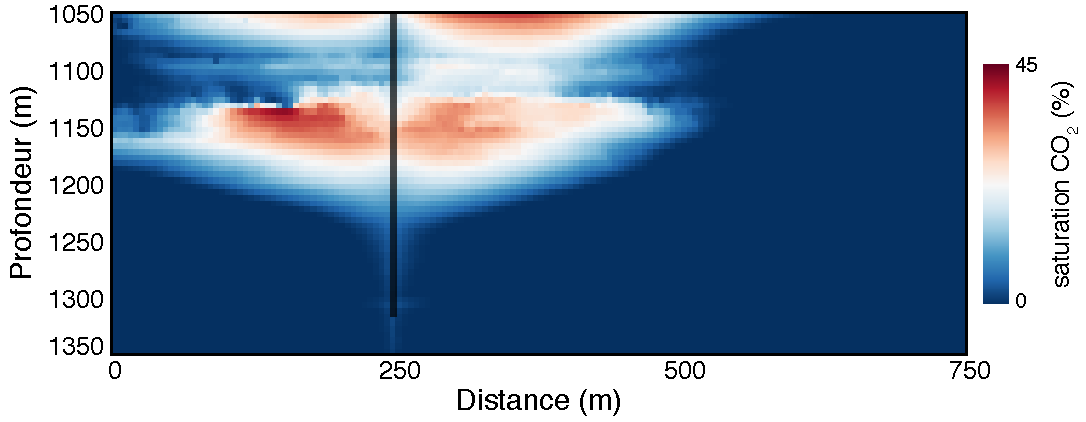
\includegraphics[width=\textwidth]{fig/CO2_ref.pdf}
                \label{fig:CO2_ref}
        \end{subfigure}%

        \begin{subfigure}[b]{0.7\textwidth}
                \caption{Réalisation stochastique aléatoire initiale}
                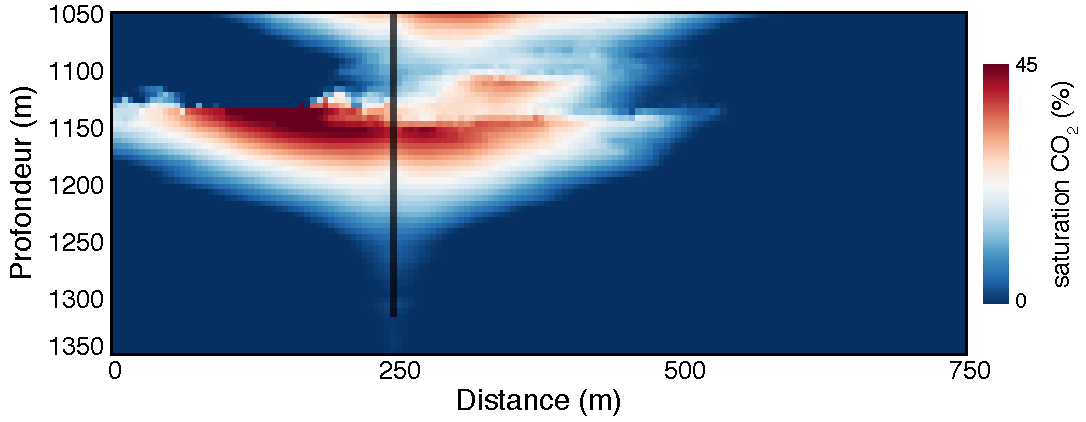
\includegraphics[width=\textwidth]{fig/CO2_real.pdf}
                \label{fig:CO_real}
        \end{subfigure}

        \begin{subfigure}[b]{0.7\textwidth}
                \caption{Modèle après optimisation statique et dynamique}
                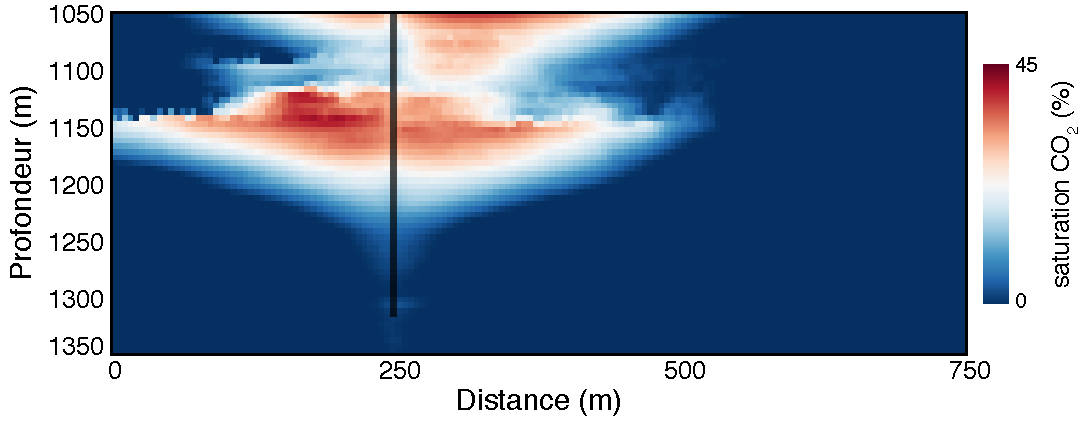
\includegraphics[width=\textwidth]{fig/CO2_dg.pdf}
                \label{fig:CO2_dg}
        \end{subfigure}
        \caption{Distribution du panache de \ce{CO2} après \num{200} jours
d'injection.}
        \label{fig:CO2_dist}
\end{figure}
\subsubsection{Transformation pétrophysique}
Les propriétés élastiques sont calculées avec des modèles pétrophysiques. Ces
modèles sont des équations qui transforment les variables pétrophysiques, telles
que porosité, minéralogie et saturation en fluide, en propriétés élastiques
telles que vitesse des ondes $P$ et $S$ et densité. Les propriétés élastiques de
la phase solides sont obtenues en appliquant la moyenne arithmétique des limites
supérieure et inférieure de Hashin-Shtrikman \citep{Hashin1963}. Ensuite, les
propriétés élastiques de la phase fluide sont dérivées en utilisant les lois de
mélange de fluides \citep{Grana2012}. Les nouvelles propriétés de la roche
saturée en \ce{CO2} sont finalement obtenues avec la relation de Gassmann
\citet{Gassmann}. La \cref{sc:elasticproperties} de l'article II à la
\cpageref{sc:elasticproperties} décrit plus en détail les équations utilisées
pour les transformations pétrophysiques ainsi que la relation de Gassmann.
\subsection{Validation du modèle}
Afin d'évaluer l'efficacité de la méthodologie proposée, des analyses
statistiques sont nécessaires. La \cref{fig:corr_a} montre la corrélation entre
le modèle de référence et une réalisation stochastique initiale, tandis que la
\cref{fig:corr_b} montre la corrélation entre le modèle de référence et le
modèle obtenu après optimisation statique et dynamique pour la vitesse des ondes $S$.
\begin{figure}[!ht]
        \centering
        \begin{subfigure}[b]{0.4\textwidth}
                \caption{Réalisation stochastique initiale}
                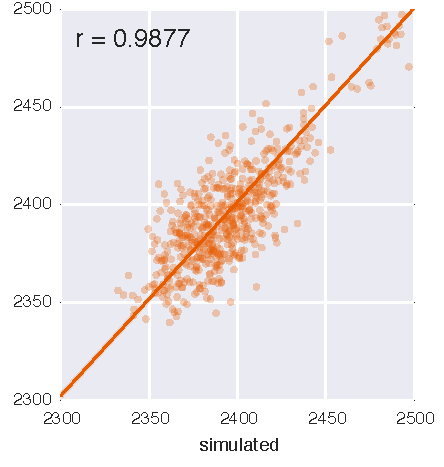
\includegraphics[width=\textwidth]{fig/corr_a.pdf}
                \label{fig:corr_a}
        \end{subfigure}%
        \begin{subfigure}[b]{0.4\textwidth}
                \caption{Optimisation statique/dynamique}
                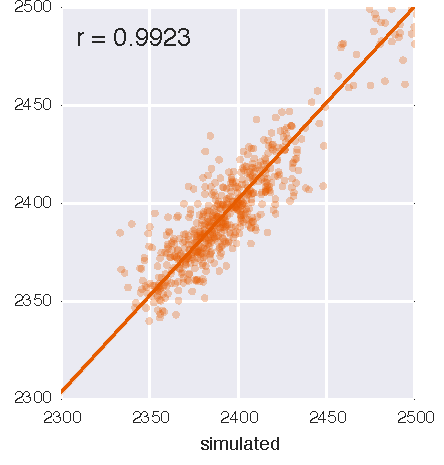
\includegraphics[width=\textwidth]{fig/corr_b.pdf}
                \label{fig:corr_b}
        \end{subfigure}
        \caption{Corrélation de la valeur de densité entre le modèle de
référence et a) 1 réalisation stochastique initiale; b) le modèle obtenu après
optimisation statique/dynamique.}
        \label{fig:corr_rho}
\end{figure}
La corrélation avec le modèle de référence est déjà très bonne après la première
étape du flux de travail (r = \num{0.9877}). Après l'optimisation statique et
dynamique, la corrélation est légèrement améliorée (r = \num{0.9923}). Les
corrélations pour $V_p$, $V_s$ et $\phi$ montrent les mêmes résultats et sont
montrées à la \cref{fig:correlation} de l'article II à la
\cpageref{fig:correlation}.\\
La \cref{fig:qqplot_2} montre le diagramme Quantile-Quantile pour la
distribution de la porosité obtenue à la fin du flux de travail avec la
distribution de la porosité du modèle de référence. Cet outil nous permet de
comparer deux distributions que l'on estime semblables. Dans le cas spécifique,
le diagramme montre un bon alignement avec la première bissectrice, qui indique
la présence d'une identité de loi entre les deux distributions
\citep{Dagnelie2011}.
\begin{figure}[!ht]
\centering
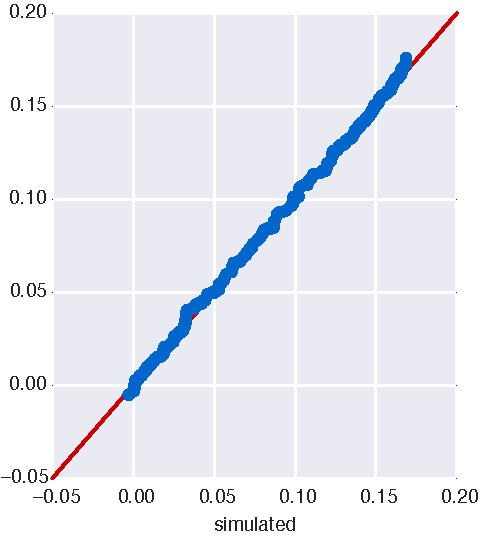
\includegraphics[width=0.4\textwidth]{fig/qqplot_2.pdf}
\caption{Graphique QQ des valeurs de porosité entre le modèle de référence et le
modèle après optimisation statique/dynamique.}
\label{fig:qqplot_2}
\end{figure}
Les diagrammes Quantile-Quantile pour $V_p$, $V_s$ et $\phi$ sont montrés à la
\cref{fig:qqplot} de l'article II à la \cpageref{fig:qqplot} et montrent un bon
alignement avec la première bissectrice, donc une identité de loi entre les
distributions des modèles finaux avec les modèles de référence. \\

Récemment, une mesure de similarité qui compare la tendance structurale locale
entre deux images (SSIM) a été développée par \citet{Wang2004}. La valeur SSIM
est comprise entre \numlist{0;1}, où \num{1} indique que les deux images sont
identiques. La \cref{fig:SSIM_2} compare le modèle de référence avec une
réalisation stochastique initiale (\cref{fig:SSIM_a}) et avec le modèle obtenu
après optimisation (\cref{fig:SSIM_b}) pour la vitesse des ondes $S$ et la
porosité.
\begin{figure}[!ht]
        \centering
        \begin{subfigure}[b]{0.35\textwidth}
                \caption{Réalisation stochastique initiale}
                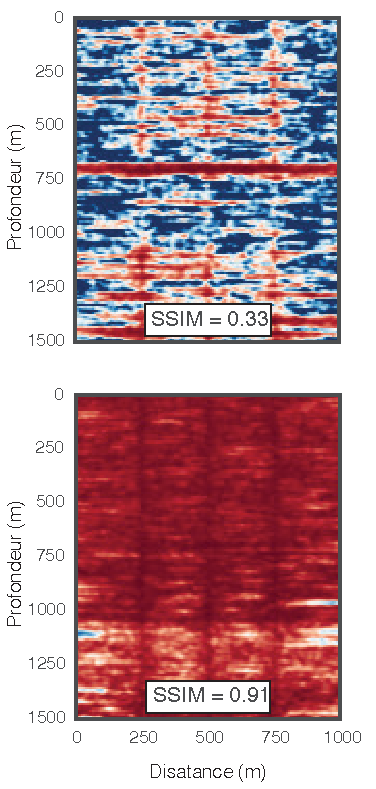
\includegraphics[width=\textwidth]{fig/SSIM_2_a.pdf}
                \label{fig:SSIM_a}
        \end{subfigure}%
        \begin{subfigure}[b]{0.412\textwidth}
                \caption{Optimisation statique/dynamique}
                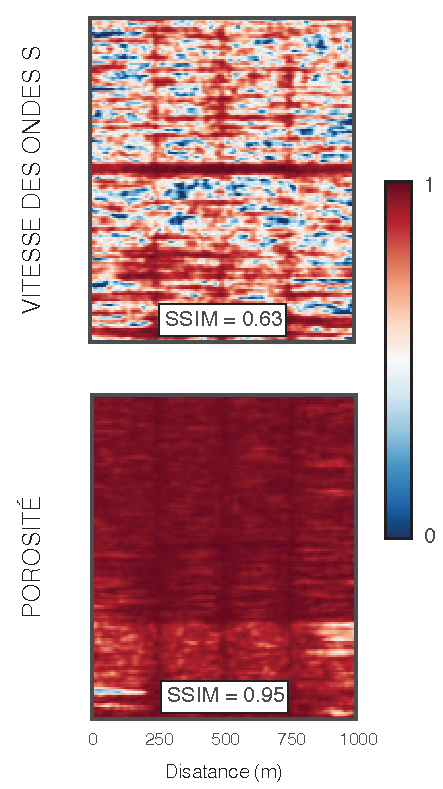
\includegraphics[width=\textwidth]{fig/SSIM_2_b.pdf}
                \label{fig:SSIM_b}
        \end{subfigure}
        \caption{SSIM index pour les vitesses des ondes $S$ et la porosité entre
le modèle de référence et a) une réalisation stochastique initiale; b) le modèle
obtenu après optimisation statique/dynamique. La valeur dans l'encadré
correspond à la valeur SSIM moyenne.}
        \label{fig:SSIM_2}
\end{figure}
Le modèle de vitesses des ondes $S$ obtenu après optimisation statique et
dynamique a une similarité avec le modèle de référence deux fois plus grande
en comparaison avec une réalisation initiale. Ce constat est aussi valable pour les
modèles de vitesse des ondes $P$ et la densité, présentés dans la
\cref{fig:SSIM} de l'article II à la \cpageref{fig:SSIM}. Il est intéressant de
noter que le long des forages utilisés pour générer les modèles initiaux
(\numlist{250;500;750}, l'index se rapproche à \num{1}. Ceci est vrai autant
pour les modèles optimisés que pour les modèles stochastiques initiaux. En
effet, les modèles initiaux sont générés en utilisant un algorithme de
cosimulation séquentielle gaussienne qui, par construction, a la caractéristique
de reproduire les observations des puits, c'est-à-dire les données de référence.
On
peut également noter une zone avec un index SSIM très élevée autour de
\SI{750}{\metre} de profondeur et qui correspond à la fine couche des argiles de
la Formation Utica. Comme montré dans la \cref{fig:well-log} de l'article II à
la \cref{fig:well-log}, les distributions des paramètres au niveau de la
Formation Utica sont très proches de la valeur centrale, qui se traduit en une
très faible variabilité et donc un degré de similitude élevée entre les
différents modèles. Ce discours n’est pas valable pour les données de porosité
(\cref{fig:SSIM_b}) qui montrent une valeur moyenne de SSIM très élevée déjà
pour les
réalisations stochastiques initiales. On peut expliquer ceci par le faible
écart-type des distributions de porosité.\\

Enfin, la simulation d’écoulement de \ce{CO2} dans le modèle obtenu après une
réalisation stochastique initiale et dans le modèle obtenu après optimisation statique et dynamique 
est effectuée afin de les comparer avec l'écoulement de \ce{CO2} dans le modèle
de référence. La \cref{fig:CO2_dist} montre l'étendue du panache de \ce{CO2}
pour les trois modèles, tandis que la \cref{fig:SSIM_intro} montre l'index de
similarité structurale entre le modèle de référence et une réalisation initiale
(\cref{fig:SSIM_real}) et entre le modèle de référence et le modèle final
(\cref{fig:SSIM_dg}).
\begin{figure}[!ht]
        \centering
        \begin{subfigure}[b]{0.7\textwidth}
                \caption{Réalisation stochastique initiale}
                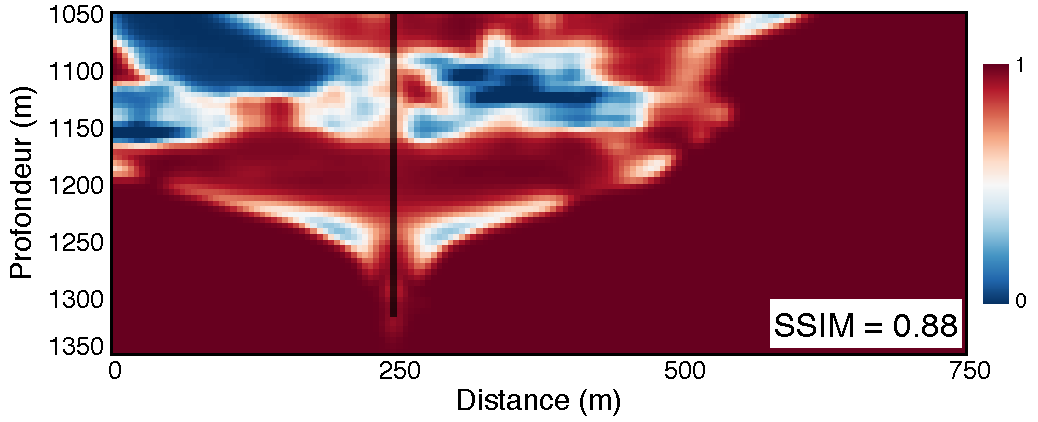
\includegraphics[width=\textwidth]{fig/SSIM_real.pdf}
                \label{fig:SSIM_real}
        \end{subfigure}%

        \begin{subfigure}[b]{0.7\textwidth}
                \caption{Modèle obtenu après optimisation statique et dynamique}
                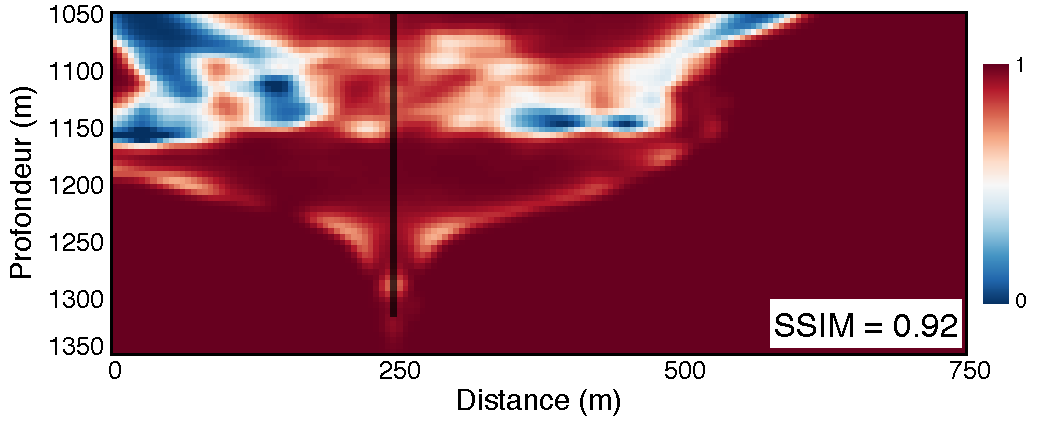
\includegraphics[width=\textwidth]{fig/SSIM_dg.pdf}
                \label{fig:SSIM_dg}
        \end{subfigure}
        \caption{Index de similarité structurelle \citep{Wang2004} du panache du
\ce{CO2} pour la simulation d’écoulement entre le modèle de référence et 1) une
réalisation stochastique initiale; 2) le modèle obtenu après optimisation
statique et dynamique.}
        \label{fig:SSIM_intro}.
\end{figure}
Le degré de similarité, bien que très élevé déjà après une réalisation
stochastique initiale (SSIM = \num{0.88}), est amélioré après l'inversion
stochastique (SSIM = \num{0.92}).
\section{Synthèse des résultats}
Cette section présente une synthèse des résultats obtenus, qui sont discutés
plus
en détail dans l'article II.
Les analyses statistiques présentées dans la section précédente montrent que le
flux de travail proposé permet d'obtenir un modèle final qui montre la meilleure
correspondance
sismique avec le modèle de référence. De plus, l'intégration de la simulation
d'écoulement dans le processus d'optimisation permet d'obtenir le modèle qui
présente la distribution du panache de \ce{CO2} la plus fidèle à la réalité. \\
La méthodologie a été appliquée à un cas synthétique où le modèle de référence a
été obtenu par cosimulation séquentielle gaussienne des données de forages
disponibles dans la zone d'étude et les modèles stochastiques initiaux sont
simulés à partir de trois forages hypothétiques du modèle de référence. Ceci
implique que le modèle de référence et les simulations stochastiques initiales
ont un degré de variabilité limitée, comme il est confirmé par leur corrélation
élevé.\\
Une étape importante pour vérifier l’efficacité de cette méthodologie est donc
l'application à un cas réel qui pourrait confirmer que l'approche proposée
améliore de façon significative l'estimation des paramètres élastiques du
réservoir.

% \chapter{Résultats et discussion}


%!TeX root = Thesis_LP.tex
\chapter{Conclusion}
Cette thèse propose une approche exhaustive pour la caractérisation sismique de
l'injection du \ce{CO2}, de la modélisation sismique par profilage sismique
vertical (PSV) à l'optimisation stochastique des propriétés élastiques du
réservoir basée sur les simulations d'écoulement. Les principaux développements
méthodologiques ciblant ces différents aspects ont été présentés au sein de
cette partie synthèse. L'approche présentée favorise l'assimilation des données
statiques (mesures de laboratoire, données de forage) avec les données dynamiques
(écoulement du \ce{CO2}).\\

Au niveau de la modélisation sismique de l'injection due \ce{CO2}, des mesures de
laboratoires ont été effectuées afin d'évaluer la réponse sismique ultrasonique du
à l'injection due \ce{CO2} dans deux échantillons du réservoir ciblé pour le
stockage du dioxyde de carbone. \\
Un modèle stochastique calibré sur les résultats obtenus en laboratoire ainsi
que sur les données de forage disponibles dans la zone d'étude a été construit
afin d'effectuer une modélisation (PSV) poroviscoélastique avant et après
injections du \ce{CO2}. Cette approche comporte les étapes suivantes:
\begin{enumerate}[-]
\item  mesurer en laboratoire la valeur du module d'incompressibilité de la roche sèche qui est un
paramètre important dans les équations poroviscoélastiques pour la modélisation
sismique.
\item utiliser un modèle stochastique pour la modélisation sismique, permettant de
reproduire la variation naturelles de la distribution des paramètres à
l’intérieur des différentes formations géologiques et donc d'obtenir une réponse
sismique plus réaliste comparée à la réponse obtenue avec un modèle homogène par
couche;
\item utiliser l'hypothèse d'équilibre vertical, permettant la simulation rapide et
précise de l'injection et de la migration du \ce{CO2}, comparé aux méthodes
numériques classiques qui ne sont pas toujours abordables ou même possibles à
mettre en œuvre car ces dernières requièrent des efforts de calculs élevés;
\item utiliser le profilage vertical pour augmenter la résolution sismique
verticale. Ceci est particulièrement utile quand les différences de signature sismique entre les
acquisitions temporelles sont très faibles;
\item utiliser une formulation poroviscoélastique est probablement l'outil le plus
efficace pour étudier l'effet de la saturation des fluides sur la réponse
sismique car avec cette formulation, les propriétés des fluides sont directement
intégrées dans les équations et les intéractions fluides/matrices qui sont prises en compte par le module de couplage.
\end{enumerate}

Les résultats obtenus ont montré que pour un contexte tel que celui qui a été étudié,
c'est-à-dire avec des porosités et des perméabilités très faibles, les différences
dans la réponse sismique dues à l'injections du \ce{CO2} sont relativement faibles
et se résument en un délai dans le temps d'arrivée de l'onde, de l'ordre de
\SI{30}{\milli\second}. La comparaison avec un scénario optimal (avec des plus grandes porosités et des pérmeabilites) montre que malgré que le panache du \ce{CO2} reste confiné autour du puits d'injection, la réponse sismique est comparable.\\
L'analyse de la variation des amplitudes avec le déport
des tirs a été faite uniquement avec des déports courts car l'apparition d'une onde
réfractée pour les déport supérieurs à \SI{700}{\metre} a empêché la séparation de
ondes ascendantes des ondes descendantes. Il va sans dire qu'il reste des idées
de recherche à poursuivre:
\begin{enumerate}[-]
\item mesurer les effets de la pression dû à l'injection du \ce{CO2} en
laboratoire et les transposer à l'échelle du réservoir afin de pouvoir les séparer
des effet dus à la substitution de fluide;
\item appliquer la méthodologie à des données réelles;
\item adapter cette méthodologie pour des scénarios 3D.
\end{enumerate}
\vspace{10 mm}
Concernant la modélisation stochastique d'un réservoir potentiel pour la
séquestration géologique du \ce{CO2}, une approche en trois étapes à été proposée
pour l'optimisation des modèles de réservoir, basées sur les données statiques
(c'est-à-dire les données de forages) et les données dynamiques (c'est-à-dire la simulation
d'écoulement du \ce{CO2}). Quelques constats peuvent être fait à cet égard:
\begin{enumerate}[-]
\item l'utilisation des données dynamiques pour la caractérisation de réservoir
pour la séquestration du \ce{CO2} apporte un bénéfice majeur pour l'obtention
d'un modèle final optimal;
\item la modélisation de l'onde complète pour plusieurs déports à court, moyen
et longue distances permet de tenir compte de toutes les variations dues à l'injection
du \ce{CO2};
\item l'utilisation d'un processeur graphique (GPU) pour la modélisation sismique à
chaque itération permet de réduire considérablement (\num{2} ordres de
grandeurs) les temps de calculs.
\end{enumerate}

Les résultats obtenus ont montré que l'utilisation des données dynamiques
dans la boucle d'optimisation permet d'améliorer la correspondance sismique du
modèle de réservoir simulé avec le modèle de référence. Cependant des
développements futurs qui permettront d'accroître sa portée sont envisageables:
\begin{enumerate}[-]
\item cette approche a été uniquement testée avec un modèle synthétique réaliste.
Son application à des données réelles permettrait de valider l'approche;
\item adapter cette méthodologie pour des scénario 3D.
\end{enumerate}

\renewcommand{\bibname}{Références}
\addcontentsline{toc}{chapter}{\bibname}
% \bibliographystyle{bibliostyleINRS}
% \bibliography{biblio/synthese.bib}
\begin{singlespacing}
\putbib[biblio/biblio]
\end{singlespacing}
\end{bibunit}
\cftaddtitleline{lof}{chapter}{Deuxième partie - Articles}{}
\cftaddtitleline{lot}{chapter}{Deuxième partie - Articles}{}
\cftaddtitleline{lof}{chapter}{Article I}{}
\cftaddtitleline{lot}{chapter}{Article I}{}
% Omettre si thèse/mémoire traditionnel
\part{Articles}


\renewcommand{\chaptername}{Article} % Afficher "Article" plutôt que "Chapitre".
\setcounter{chapter}{0} % Recommencer la numérotation des chapitres.
\cftaddtitleline{lof}{chapter}{Article II}{}
\cftaddtitleline{lot}{chapter}{Article II}{}

\begin{bibunit}[bibliostyleINRS]
% \begin{spacing}{1.5}
%!TeX root = Thesis_LP.tex
% \sisetup{
% list-final-separator= { and },    % Place "et" à la fin de la liste
% range-phrase= { to }             % Place "à" à entre la gamm
% }
\pagestyle{fancy}
\fancyhf{}
\renewcommand{\headrulewidth}{0pt}
\fancyhead[LO]{\emph{Article 1. VSP modeling for \ce{CO2} monitoring}}
\fancyhead[RO]{\thepage}
\fancyhead[LE]{\thepage}

\chapter{Sensitivity of vertical seismic profiling for monitoring
\texorpdfstring{\ce{CO2}}{CO2} storage in a low porosity reservoir - An example
from the St-Lawrence Lowlands, Canada}

\label{ch:article1}
\selectlanguage{english}

\chaptermark{Sensintivity of VSP for \ce{CO2} monitoring} % Titre court
% apparaissant dans l'entête des pages

{\setlength{\parindent}{0cm}
\underline{\textbf{Titre traduit}}\\
Sensibilité du profilage sismique vertical pour la surveillance du  \ce{CO2}
stocké dans un réservoir peu poreux - Exemple des Basses Terres du St Laurent,
Canada

\underline{\textbf{Auteurs}}\\
Lorenzo Perozzi$^1$, Bernard Giroux$^1$, Douglas R. Schmitt$^2$, Randolf S.
Kofman$^2$\\
$^1$ Institut national de la recherche scientifique - Centre Eau Terre
Environnement, 490, de la Couronne, Qu\'ebec, QC, G1K 9A9, CANADA\\
$^2$ Department of Physics, Institute for Geophysical Research, CCIS 4-183,
University of Alberta, Edmonton, AB, T6G 2E1, CANADA

\newpage
\underline{\textbf{Contribution}}
{\setstretch{1.0}
\begin{description}[leftmargin=!,labelwidth=\widthof{\bfseries Randolf S.
Kofman}]
  \setlength\itemsep{0.7em}
  \item[Lorenzo Perozzi] Conceptualisé et réalisé (les mesures de laboratoire,
la modélisation sismique, l’interprétation des résultats) l’étude et rédigé
l’article
  \item[Bernard Giroux]  Conceptualisé l'étude, fourni des conseils sur
l’interprétation des résultats et contribué à la rédaction de l’article.
  \item[Douglas R. Schmitt]  Contribué à la rédaction de l’article
  \item[Randolf S. Kofman]  Fourni de conseils et realisé une partie de mesures
de laboratoire.\\
\end{description}
}


\underline{\textbf{Publication ciblée}}\\
{\setstretch{0.5}
International Journal of Greenhouse Gas Control\\
Première soumission: 6 janvier 2015\\
Soumission après révision: 26 juillet 2015
}


\underline{\textbf{Résumé traduit}}\\
Nous avons réalisé une série de mesures sismiques de laboratoire sous
differentes conditions de pressions et temperature afin de tester la réponse
sismique sur deux échantillons saturés en \ce{CO2} provenant du reservoir des
Basses Terre du Saint Laurent. Les resultats ont montré que la vitesse et
l'amplitude du signal sismique peuvent être utilisées pour detecter le changement
de phase du \ce{CO2}. Les resultats ont aussi servi a calibrer un modèle
géologique héterogène à partir duquel des séismogrammes de profilage sismique vertical ont été générés. Le degré de saturation  autour d'un puits
d'injection a été calculé pour un periode de  \num{50} ans qui inclut
un periode d'injection de \num{15} ans suivie par \num{35} de migration de
\ce{CO2}. Des seismogrammes synthetiques de profilage sismique vertical dans le
temps ont été générés après 5, 15 et 50 ans d'injection. Les resultats ont montré que le
remplacement de la saumure par le \ce{CO2} provoque un délai en temps des
reflecteurs situés au-dessous du reservoir, malgrés ses faibles porosités et
perméabilités. La comparaison entre un modèle homogène classique et le modèle
hétérogène proposé dans ce travail montre que le modèle homogène classique
pourrait conduire à une mauvaise interpretation de l'effet du \ce{CO2} sur la
réponse sismique.
}

\section{Abstract}
We have performed a series of rock physics measurements under various simulated
confining and pore pressure and temperature states to test the seismic response
of two low permeability reservoir samples of the St.\ Lawrence Lowlands
sedimentary basin to different \ce{CO2} phases. Results show that the seismic
velocity and amplitude can be used to detect the \ce{CO2} phase transition. The
laboratory measurements calibrated a heterogeneous geological model from which
synthetic vertical seismic profile (VSP) seismograms were generated. The
saturation states around a single injection point in the geological model were
calculated over a \num{50} year time period which included constant rate
injection for the first \num{15} years followed by \num{35} years of \ce{CO2}
migration. Synthetic time-lapse VSP seismograms were produced after
\numlist{5;15;50} years from the start of injection. Results show that
substitution of brine by \ce{CO2} delays the times of seismic reflection events
below the target reservoir despite its low reservoir permeabilities and
porosities. A comparison between a classical blocky model and our heterogeneous
model shows that the blocky model leads to a misinterpretation of the \ce{CO2}
effects on the seismic response.
\section{Introduction}
The measurement, monitoring and verification (MMV) of geological \ce{CO2}
storage is essential for ensuring storage integrity and social acceptance of
Carbon Capture and Storage (CCS). Satisfying these societal requirements is
necessary to allow the deployment of the MMV technologies at a scale sufficient
to reduce the rate of increase of anthropogenically produced \ce{CO2}. Also, in
a carbon market context, appraisal and verification of stored \ce{CO2} should be
integrated components of CCS projects. As such, monitoring programs of \ce{CO2}
injection should ultimately allow for the quantitative estimation of \ce{CO2}
saturation throughout the reservoir and watch for any migration of carbon
dioxide into surrounding geological formations. Geophysical methods are
challenged in this respect, and multi-method approaches should be favored.
Gravity monitoring can be helpful for mass balance estimation, especially if
downhole gravimeters can be positioned close to the reservoir \citep{dodds13}.
Electrical methods can also play an important role due to the very low
sensitivity of electrical properties to pressure effects and high sensitivity to
pore fluid conductivity \citep{schon04,SchmidtHattenberger2013}. \\
To date, active source seismic methods remain the principal geophysical method
of all monitoring programs. Indeed, seismic methods were shown to be efficient
for MMV due to their high resolution and their sensitivity to porosity and fluid
saturation \citep{White2013a,Lumley2010a,Lumley2010,Carcione2006}.
Nevertheless, there can be a great deal of ambiguity in the quantitative
interpretation of observed seismic responses. Proper interpretation requires
that workers understand how seismic reflectivity will evolve with changes in the
effective stress, temperature, and state of saturation within the subsurface.
Despite these issues it is likely that active-source seismic methods will always
play a central part in \ce{CO2} monitoring programs due to their high resolution
compared to other geophysical methods. Consequently responsible operators will
need to properly understand the effects of \ce{CO2} on seismic properties. \\
% Since \num{2008}, the INRS \ce{CO2} research chair granted by the Minist\`ere
% du D\'e\-ve\-loppe\-ment durable, de l'Environnement et des Parcs du Qu\'ebec,
% studies the feasibility of geological storage of \ce{CO2} in the province of
% Quebec, Canada.  As part of the research program of the Chair, an assessment of
% the performance of seismic monitoring is carried out for in the particular
% context of the St.\ Lawrence Lowlands.\\
The Cambrian-Ordovician sedimentary basin of the St.\ Lawrence Platform in
southern Quebec, Canada, has been identified as the most prospective basin for
\ce{CO2} storage in the province \citep{Malo2012}. The Bécancour region is
located on the south shore of the St.\ Lawrence River, midway between Montreal
and Quebec City (\Cref{fig:map}). The Bé\-can\-cour region's deep saline
aquifers were selected as a potential target for injection of \ce{CO2} in a
future pilot project. This selection was based on seismic reflection and well
log data available from gas exploration, and based on the proximity of an
industrial zone emitting up to \SI{1}{\mega\tonne} of \ce{CO2} per year. The
success of the storage depends on the capability to monitor movements of the
injected gas into the subsurface. As in all current CCS projects, seismic
methods are an important component of the monitoring program at Bécancour. In
such projects, prior estimation of elastic property changes in response to the
injection of \ce{CO2} is crucial to perform proper monitoring and subsequent
interpretation of the time-lapse seismic data. There is thus a mandatory need to
understand how injected \ce{CO2} influences seismic response and how seismic
methods could obtain reliable quantitative estimates of injected \ce{CO2}
\citep{White2013}.\\
\begin{figure}[!ht]
        \centering
        \begin{subfigure}[b]{.55\textwidth}
                \caption{Distribution of sedimentary basins on the south shore
of the St. Lawrence River. Bottom right inset is the distribution of deep saline
aquifers in Canada \citep{Wright2013}.}
                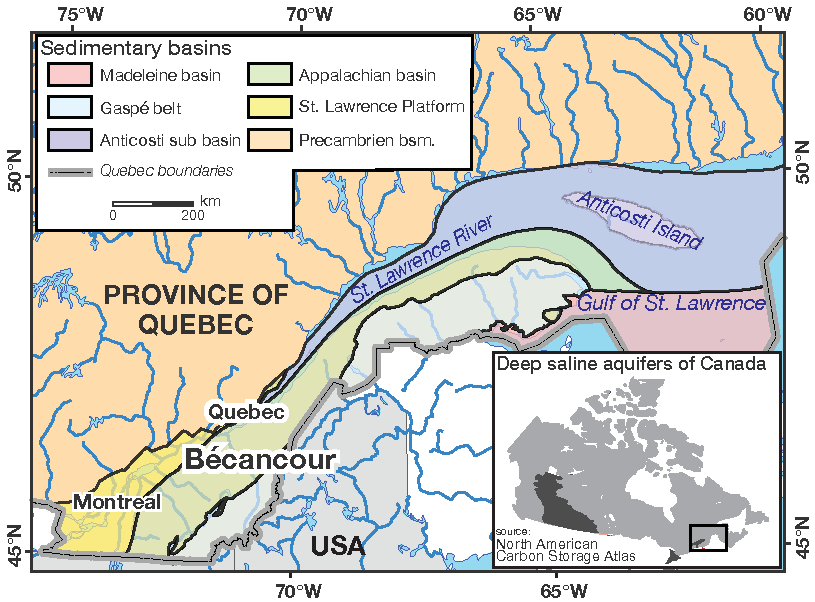
\includegraphics[width=\textwidth]{fig/map.pdf}
                \label{fig:map}
        \end{subfigure}%

        \begin{subfigure}[b]{.55\textwidth}
                \caption{Simplified stratigraphy of the St. Lawrence Platform.}
                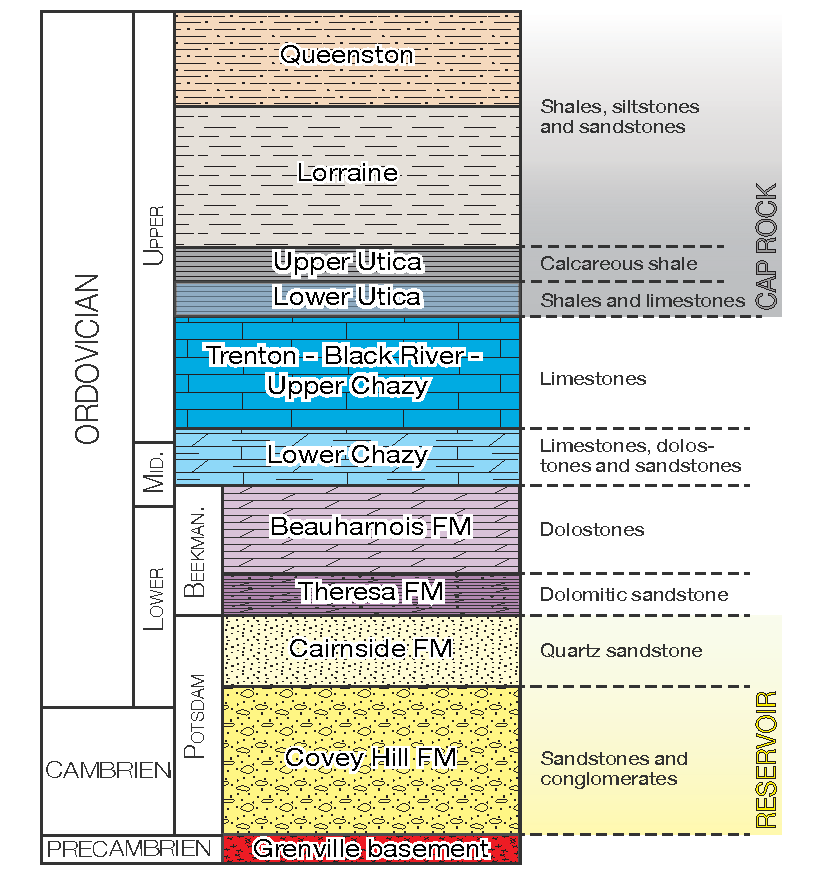
\includegraphics[width=\textwidth]{fig/strati.pdf}
                \label{fig:strati}
        \end{subfigure}

        \caption{Geographical and stratigraphical map of the studied area.
Modified from \citep{Malo2012} and  \citep{Claprood2012}}
        \label{fig:geo}.
\end{figure}
The aim of this study is to better understand the dependence of the seismic
properties on the porosity, mineralogy and pore fluids found in the
Bé\-can\-cour reservoir through both laboratory measurements and numerical
modeling.  In this contribution, we first present a set of laboratory
measurements of the compressional ($P$) and shear ($S$) wave velocity and
amplitude made on two sandstone samples from the target reservoir, fully
saturated with \ce{CO2} at different temperatures and pressures. The results of
these experiments are then used to build a geological model and generate
synthetic seismograms forecasting the response to \ce{CO2} injection in the
reservoir formations.
\section{Bécancour reservoir properties}
The St.\ Lawrence Lowlands sedimentary basin is located between the Precambrian
Grenville basement in the north-west and the Appalachian thrust domain in the
south-east (\Cref{fig:map}). The Paleozoic sedimentary succession of the St.\
Lawrence Platform is shown in \cref{fig:strati}. The Potsdam Group lies
unconformably upon the metamorphic Precambrian Grenville basement. It is
comprised of the Covey Hill (Cambrian sandstones and conglomerates) and the
Cairnside (lower Ordovician quartz sandstone) formations. The remainder of the
section is all of Ordovician age. The Beekmantown Group includes the Theresa
(dolomitic sandstones) and the Beau\-har\-nois (dolostones) formations. The
lower Chazy unit is composed of limestones, dolostones, and sandstones. The
Trenton, Black River, and upper Chazy groups, are limestones. The Trenton Group
is overlain by the Utica Shale and several hundred meters of interbedded shales,
siltstones and sandstones of the Lorraine Group. The lower Utica Shale comprises
limestone beds and is more calcareous than the upper Utica Shale. Deep saline
aquifers are found in the Trenton, Beekmantown and Potsdam Groups.\\
The Covey Hill sandstone (lower Potsdam) appears as the most suitable saline
aquifer for \ce{CO2} injection/storage. This unit has the largest injectable
pore volume due to highest porosity (\SI{6}{\percent}), net pay thickness
(\SI{196}{\metre}), highest matrix permeability (\SI{2.4e-16}{\metre\squared})
and lowest salinity (\SI[per-mode=symbol]{108.500}{\milli\gram\per\litre}) that
may assure feasible injectivity.
The sandstones of the Covey Hill formation are located at depths of
\SIrange{1100}{1400}{\metre} where injected \ce{CO2} would be in a supercritical
state that has lower density and viscosity than the liquid brine it displaces.\\
The \ce{CO2} can also be injected in the Cairnside (upper Potsdam), however its
lower permeability, lower porosity and more saline waters are less favorable for
the storage of \ce{CO2} \citep{TranNgoc2014}. Moreover, the temperature gradient
of Bé\-can\-cour reservoir (\SI[multi-part-units =
single]{23.5(6)}{\degreeCelsius\per\km}) may not lead to a supercritical state
of \ce{CO2} everywhere in the Cairnside Formation, due to the shallower depth of
its formation top \citep{Claprood2012}.\\
The regional caprock unit consists of the Utica and Lorraine shales. The
thickness (\SI{>800}{\metre}) and permeability (\SI{1e-19}{\metre\squared}) of
the caprock units in the Bé\-can\-cour region are apparently capable of
preventing buoyancy-driven migration of injected \ce{CO2} to the surface, as
they have maintained over-pressured conditions in the saline aquifers
\citep{TranNgoc2014}. Petrophysical and hydrogeological properties of the
reservoir are summarized in Table~\cref{tbl:prop}.
\begin{table}[tpb]
	\caption{Physical properties of the Potsdam group reservoir and the
Utica/Lorraine cap-rock.}
	\label{tbl:prop}
	\sisetup{per-mode = symbol,table-format = 1.2e-2}
    \centering
    \begin{threeparttable}[b]
        \begin{tabular}{ll@{\hspace{2em}}
        S[table-comparator = true,table-format = 1.0e-2]
        @{\hspace{3em}}
        S
        @{\hspace{3em}}
        S[table-format = 1.1e-2]
        }
            \toprule
            &&  & \multicolumn{2}{c}{Potsdam Group}\\
            \cmidrule(r){4-5}
             && {Cap Rock} & {Cairnside} & {Covey Hill} \\
	        % \cmidrule(r){3-5}
            \midrule
	        {Lithology} && {shale}  & {sandstone} & {sandstone} \\
			Grain density& (\si{\gram\per\cubic\cm)}  & {2.700} & {2.632} & {2.613} \\
			Porosity\tnote{a}&  (\si{\percent}) & {4} & {3.35} & {6}      \\
			Matrix permeability\tnote{b}& (\si{\metre\squared}) & 4e-19& 1.2e-16
&2.5e-4\\
			Horizontal permeability\tnote{a}& (\si{\metre\squared}) & n/a & 8.89e-15 &
8.9e-16\\
			Vertical permeability\tnote{a}& (\si{\metre\squared}) & n/a & 6e-17 &
1.2e-16\\
			Salinity &(\si{\milli\gram\per\litre})  & n/a & {\num{242000}} &
{\num{108500}}\\
			Net pay thickness &(\si{m}) & {> 800} & {68} & {196}\\
			Pore size &(\si{\micro\metre}) & n/a & {0.55} & {0.55}\\
			\bottomrule
        \end{tabular}
        \begin{tablenotes}\footnotesize
			\item [a] Mean values measured form core analysis, see \citet{TranNgoc2014}
for details.
			\item [b] Determined from drill stem tests, see
\citet{TranNgoc2014,TranNgoc2013}
        \end{tablenotes}
    \end{threeparttable}
\end{table}
\section{Ultrasonic measurements}
\label{sc:art_1_ultrasonic_measurements}
Laboratory measurements on core samples under \ce{CO2} flooding can be used to
calibrate seismic data. As reported by \citet{Njiekak2013}, most experiments
described in the literature so far
\citep{Wang1989,Xue2005,Lei2009,Purcell2010,Shi2011,Ivanova2012}, involve the
injection of \ce{CO2} into a porous media pre-saturated with another in situ
fluid and the acoustic variations observed are usually from a combination of
pore pressure and fluid substitution effects. However, it is difficult to apply
the results of these studies to the interpretation of seismic data since
observed velocity changes due solely to \ce{CO2} cannot be quantitatively
determined as the \ce{CO2} partial saturation of the injected fluid is generally
unknown. \citet{Yam2011b,Chowdhury2013,Njiekak2013} investigated the seismic
effects associated with the different phase states of \ce{CO2} by measuring the
ultrasonic response of Berea and Fontainbleau sandstones and carbonate samples
from the Weyburn-Midale geologic project fully saturated with \ce{CO2} at
different temperatures and confining and pore pressures. In these works,
particular attention was given to the separation of the seismic effect due to
changes in the pore fluid, from those induced by the pore pressure build-up.
\citet{Lebedev2013} similarly tested the effects of supercritical \ce{CO2}
injection into sandstones from the Otway Basin on acoustic responses.
\citet{Kitamura2014} estimated the saturation of CO$_2$ from the changes in
$S$-wave velocity during laboratory measurements of porous sandstone during
drainage and imbibition.\\
For this study, laboratory measurements were carried out at the Experimental
Geophysics Group laboratory (Institute for Geophysical Research, Department of
Physics, University of Alberta) on two representative core samples of the
Potsdam Group, following the approach proposed by \citet{Schmitt2012}.
\subsection{Sample characterization}
The Cairnside (CA) and Covey Hill (CH) samples used for ultrasonic measurements
are from well A196, located in the northeastern Bé\-can\-cour sub-reservoir.
More details about this well can be found in \citet{TranNgoc2014}. A set of
mercury injection porosimetry measurements were performed on both samples. This
analysis established the relationship between capillary pressure and fluid
saturation. From that, pore-size in the CA and CH sandstones samples were
obtained (\cref{tbl:prop}).
\subsection{Experimental apparatus and procedure}
\label{sc:experimental_apparatus}
The experimental apparatus includes several components such as the pressure
vessel to enclose and apply an hydrostatic confining pressure to the core
sample, a heat tape wrapped around the pressure vessel, tanks as pore fluids
sources, an independent Quizix\textsuperscript{\texttrademark} dual cylinder
pumping system for regulating confining and pore pressure, a JSR PR35
pulser/receiver and a digital oscilloscope for recording waveform at a sampling
rate of \SI{10}{\ns}. Some of these are highlighted in \cref{fig:apparatus}.\\
\begin{figure}[!ht]
\centering
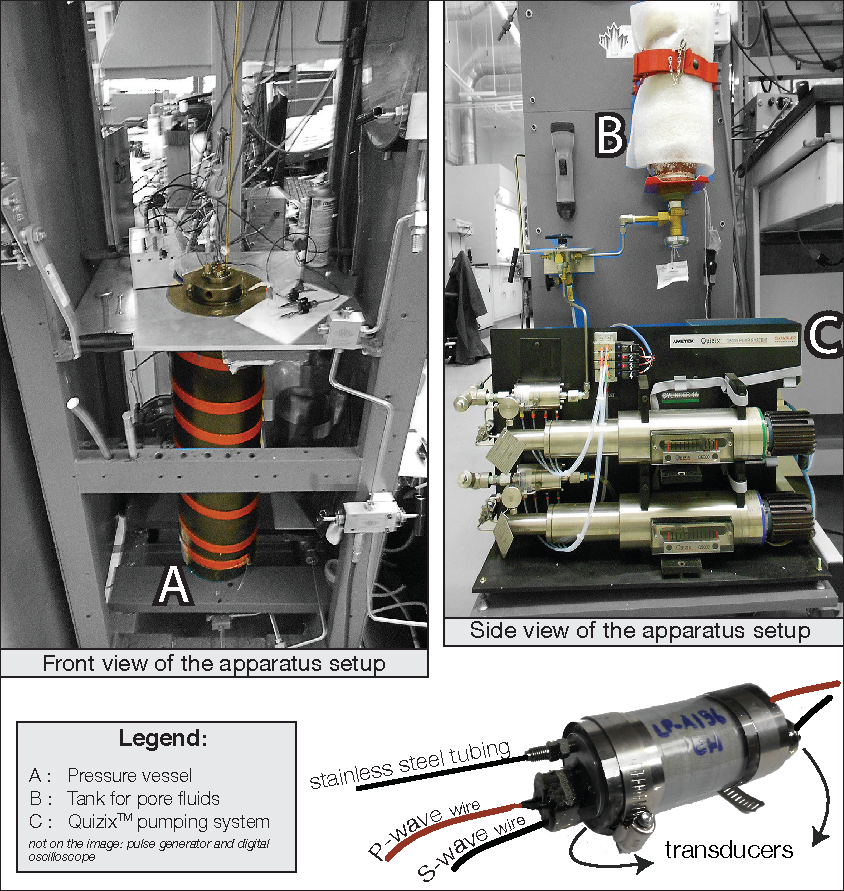
\includegraphics[width=1\textwidth]{fig/apparatus.pdf}
\caption{Apparatus setup and rock sample with transducer assemblage}
\label{fig:apparatus}
\end{figure}
Cylindrical shaped samples of \SI{3.7}{\cm} in diameter having lengths greater
than \SI{4}{\cm}, obtained from CA and CH cores, are used. The ends of the
samples are polished and made as parallel as possible using a surface grinder.
The parallelism is measured using a dial gauge and considered acceptable if it
is within \SI{\pm0.025}{\mm}. Each sample is then dried under vacuum at modest
temperatures (\SI{\sim70}{\degreeCelsius}). It is prepared for the measurement
suite by attaching the set of ultrasonic transducers to its ends. Each
transducer consists of one longitudinal mode and one transverse mode PZT ceramic
glued to an aluminum alloy buffer. The sample-transducers assembly
(\cref{fig:apparatus}) is then hermetically sealed to prevent any contamination
by the hydraulic fluid once the sample is in the pressure vessel. The assembly
is then placed inside the pressure vessel (\cref{fig:apparatus}) in a
cylindrical cavity filled with hydraulic oil. The hydraulic oil serves as the
pressurizing medium for providing hydrostatic confining pressure on the
sample.\\
The \ce{CO2} is introduced into the sample via stainless steel tubing that
connects the pore space of the sample with the pore fluid reservoir located
outside of the vessel. The transmitted seismic signal was generated by
triggering the transducer with a negative spike pulse. For detailed description
of the apparatus see \citet{Njiekak2013} and \citet{Yam2011}.
\subsection{Testing sequence}
The first set of measurements was made with pore space subject to vacuum to
provide the 'dry' properties at different temperature and pressure conditions to
evaluate their effect on the rock frame. The measurements were then repeated
with full \ce{CO2} saturation under a variety of pore pressure at
\SIlist{25;35}{\degreeCelsius} in order to sample the full range of \ce{CO2}
phase states (\cref{fig:bulkdensity}). Finally 'dry' measurements were repeated
to assess any mechanical change that might have altered the rock 'dry'
properties. For each measurements, the sample was left to equilibrate for
\num{5} minutes at constant pressure prior to acquisition of the waveforms. To
reduce random noise effects, the final waveform recorded is a sum of at least
\num{100} traces.
\begin{figure}[!ht]
        \centering
        \begin{subfigure}[b]{.5\textwidth}
                \caption{Density of \ce{CO2}}
                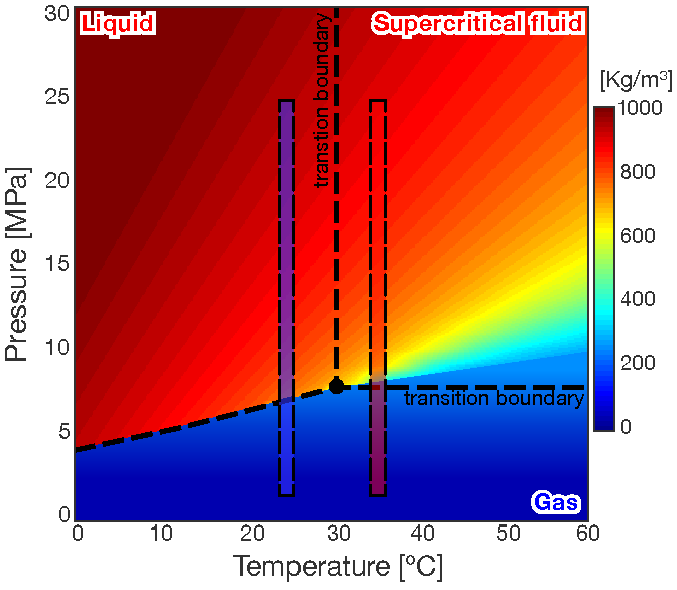
\includegraphics[width=\textwidth]{fig/density.pdf}
                \label{fig:density}
        \end{subfigure}%
        \begin{subfigure}[b]{.5\textwidth}
                \caption{Bulk modulus of \ce{CO2}}
                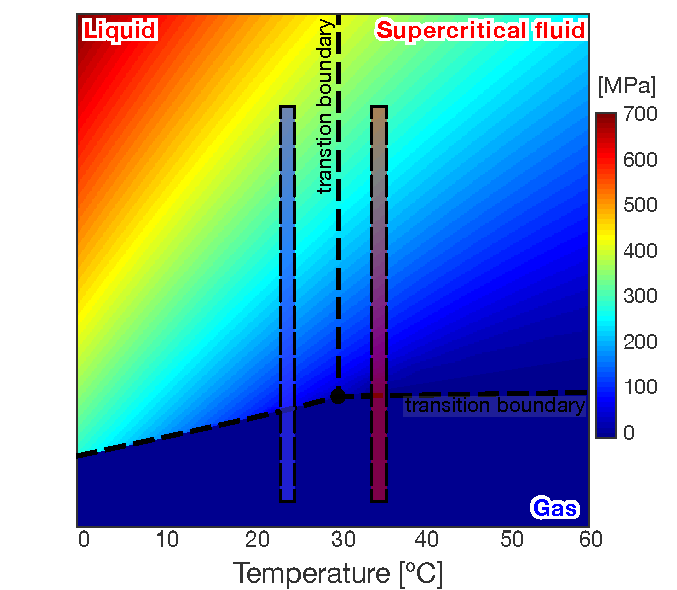
\includegraphics[width=\textwidth]{fig/bulk.pdf}
                \label{fig:bulk}
        \end{subfigure}
        \caption{Phase diagrams of \ce{CO2} based on the thermodynamic model of
\citet{Span1996}. The blue and red bars indicate the P and T conditions for the
experiments runs.}
        \label{fig:bulkdensity}
\end{figure}
\subsection{Experimental results}
An essential characteristic of the measurements was to ensure that the
variations of the waveform are linked only to the change of the properties of
fluids and not to differential pressure dependent changes in the elastic
properties of the rock's frame. Thus, all measurements were carried out at
constant differential pressure of \SI{14}{\mega\pascal} (corresponding to the
expected reservoir conditions) by varying the confining pressure and the pore
pressure according to
\begin{equation}
 P_{d} = P_{c} - P_{p},
\end{equation}
where $P_{d}$ is differential pressure, $P_{c}$ is confining pressure and
$P_{p}$ is pore pressure. As the sample is buffered by two aluminum caps, the
measured travel time must be corrected to obtain the wave velocity $\nu$ of the
sample using
\begin{equation}
 \nu = \frac{L_{s}}{t_{bs}-t_{b}},
\end{equation}
where $L_s$ is the sample length and $t_{bs} - t_{b}$ is the difference between
the travel time through the aluminum buffers and the sample $t_{bs}$, and the
traveltime through the aluminum buffer without the sample $t_b$. The buffer
transit time $t_b$ was determined before the tests that included the samples
over the range of confining pressures and temperatures expected; and this
pressure and temperature dependent values were used in correcting the observed
times through the samples.\\
We present here the measurements made for full \ce{CO2} saturation at two
constant temperature (\SIlist{25;35}{\degreeCelsius}) with the pore pressure
varying from \SIrange[range-units = single]{2}{25}{\mega\pascal} in each case.
Carbon dioxide is in a gaseous state at the lower pores pressures, and in liquid
or supercritical state at higher pore pressures, depending on the temperature as
shown in \cref{fig:bulkdensity}. The suite of $P$-waveforms for CH sample at
\SI{25}{\degreeCelsius} are shown in \cref{fig:waveform_a}.
\Cref{fig:waveform_b} shows how the signal amplitude is picked.  Wave velocities
and relative signal amplitude for $P$- and $S$-wave for the two constant
temperature runs are plotted in \cref{fig:results_lab}. In each subplot curves
for both Cairnside (red) and Covey Hill samples (yellow) are shown.
\begin{figure}[!hb]
        \centering
        \begin{subfigure}[b]{.5\textwidth}
                \caption{normalized P-waveforms over a confining pressure
varying from \SIrange[range-units = single]{2}{25}{\mega\pascal}, red line shows
the first arrival picking.}
                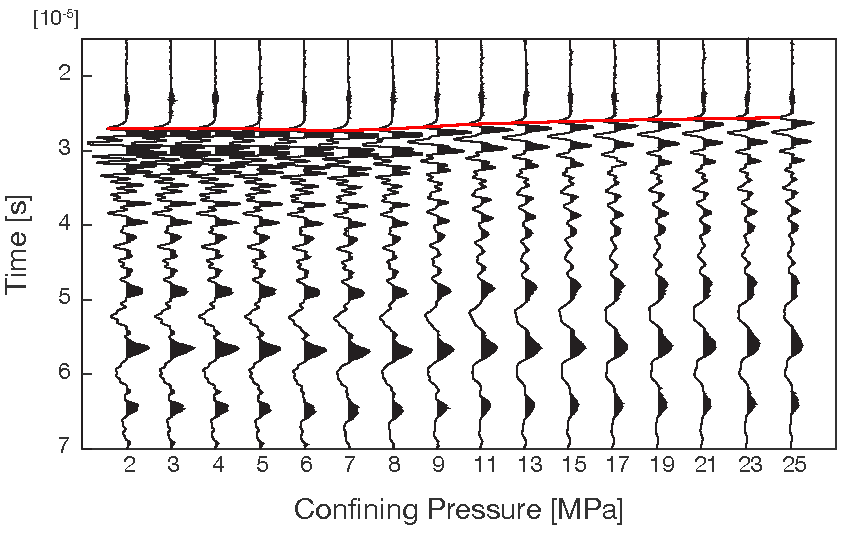
\includegraphics[width=\textwidth]{fig/waveform_a.pdf}
                \label{fig:waveform_a}
        \end{subfigure}%

        \begin{subfigure}[b]{.5\textwidth}
                \caption{Amplitude difference between $P$-waveforms at
\SIlist{2;25}{\mega\pascal}.}
                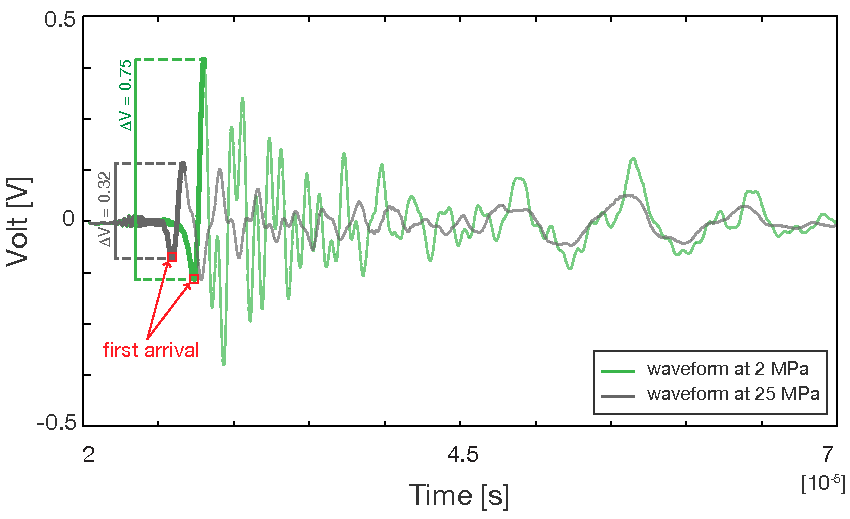
\includegraphics[width=\textwidth]{fig/waveform_b.pdf}
                \label{fig:waveform_b}
        \end{subfigure}

        \caption{P-waveforms of measurements at \SI{35}{\degreeCelsius} for the
CH sample.}
\end{figure}
\subsubsection{Velocity}
For fluid substitution with no change in matrix properties, a change in $P$-wave
velocity is expected due to the change in the saturated bulk modulus
(incompressibility), with a minimal change in $S$-wave velocity expected due to
the lack of change in shear modulus, which is a property presumed to be not
affected by pore fluid \citep{Daley2007}. The change in the bulk density of the
material due to varying \ce{CO2} fluid density is also a significant factor
affecting the wave speeds through the rock. The experimental observations are
summarized as:
\begin{enumerate}[-]
\item $P$-wave velocities (\cref{fig:results_lab_a}) initially decrease with
increasing pore pressure over the range \SIrange{2}{7}{\mega\pascal} for all
runs and for the two samples. These velocities drops are consistent with the
increase of the \ce{CO2} gas density (\cref{fig:density}) as has been observed
in \citep{Yam2011} and \citep{Chowdhury2014}.
\item Once the phase transition is crossed, velocities increase with pore
pressure for both runs. This trend is far more pronounced for the CH sample than
for the CA sample.
\item The pore fluids transition from gaseous \ce{CO2} to liquid/supercritical
\ce{CO2} only concerns $P$-wave velocity. This is confirmed by the lack of sharp
changes in the $S$-wave velocity.
\end{enumerate}
Unfortunately, brine-saturated measurements have not been done due to the salts
dissolved in water which could have damaged the pumping system. However, smooth
velocity variation under water-saturated measurements is expected since water
will not undergo any phase transition based on the applied conditions as
observed by \citet{Njiekak2013}, \citet{Yam2011} and \citet{Chowdhury2014}.
\subsubsection{Signal amplitude}
Signal amplitude (\cref{fig:results_lab_b} and \cref{fig:results_lab_d}) shows a
rapid decrease in the pressure range \SIrange[range-units =
single]{5}{7}{\mega\pascal}. Once the \ce{CO2} phase transition is crossed the
decrease is smoother. This trend is valid for CH sample for both $P$- and
$S$-wave signal, however, for the CA sample, the amplitude decreases steadily
and the phase transition is not clearly detected.\\
Despite the relatively low permeability of the samples, there are substantial
variations on velocity and signal amplitude measurements. Nevertheless, the CH
sample shows a larger sensitivity to \ce{CO2} phase change when compared to the
CA sample. This is attributed to the larger porosity and permeability of the
former (\cref{tbl:prop}).
In the next section, we explore how the higher sensitivity of the CH unit
affects the time-lapse seismic response for a VSP monitoring program.
\begin{landscape}
    \begin{figure*}[p]
        \centering
        \begin{subfigure}[b]{0.563\textwidth}
            \centering
            \caption{$P$-wave velocity}
            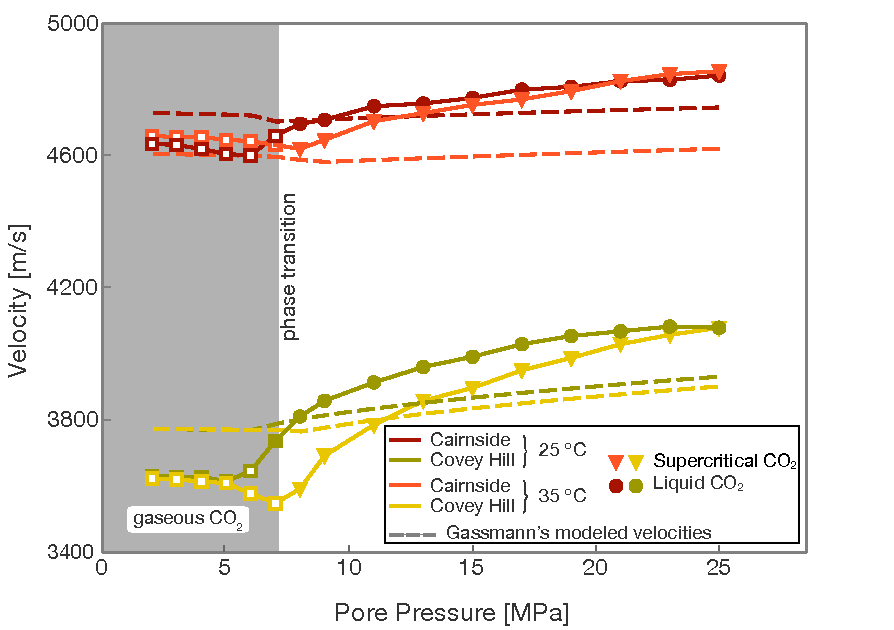
\includegraphics[width=\textwidth]{fig/results_lab_a.pdf}
            \label{fig:results_lab_a}
        \end{subfigure}
        \qquad
        \begin{subfigure}[b]{0.563\textwidth}
            \centering
            \caption{$S$-wave velocity}
            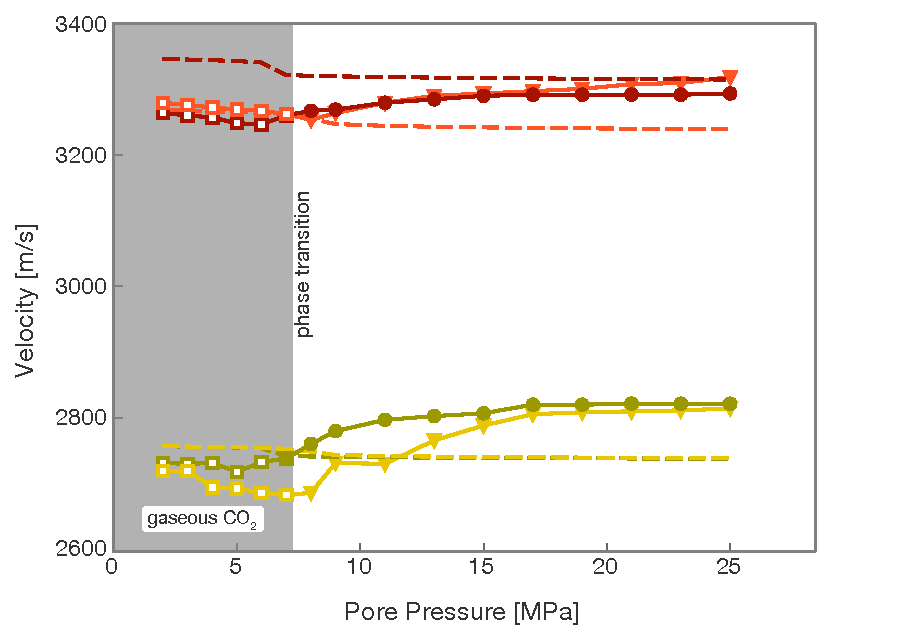
\includegraphics[width=\textwidth]{fig/results_lab_c.pdf}
            \label{fig:results_lab_c}
        \end{subfigure}
        \vskip\baselineskip
        \begin{subfigure}[b]{0.563\textwidth}
            \centering
            \caption{$S$-wave amplitude}
            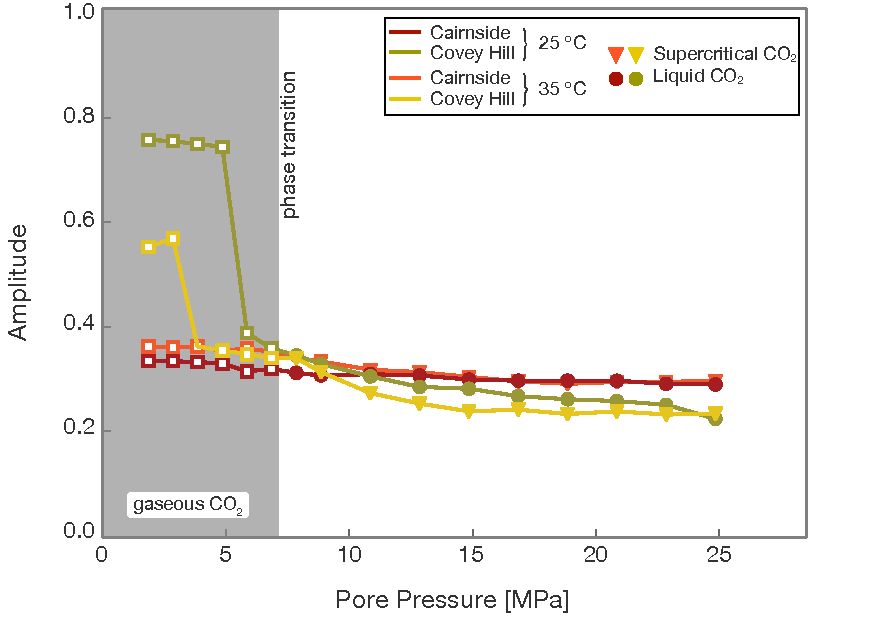
\includegraphics[width=\textwidth]{fig/results_lab_b.pdf}
            \label{fig:results_lab_b}
        \end{subfigure}
        \qquad
        \begin{subfigure}[b]{0.563\textwidth}
            \centering
            \caption{$S$-wave amplitude}
            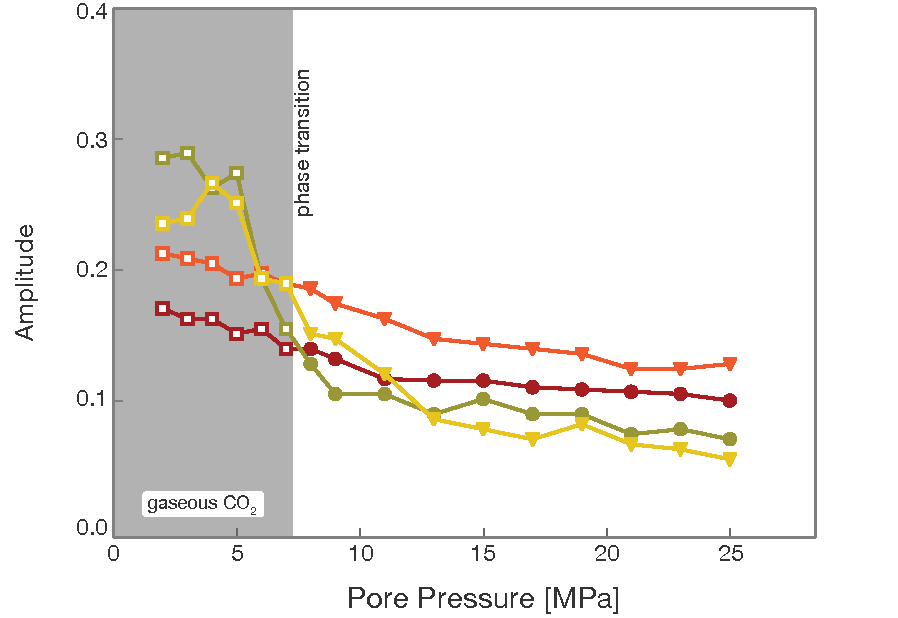
\includegraphics[width=\textwidth]{fig/results_lab_d.pdf}
            \label{fig:results_lab_d}
        \end{subfigure}
        \caption{Velocity and amplitude response for CO$_2$ injection in the
Covey Hill (yellow) and Cairnside (red) samples.}
        \label{fig:results_lab}
    \end{figure*}
\end{landscape}
\subsection{Gassmann modeling}
Applying the laboratory results to seismic monitoring will require the high
frequency data to be scaled down to low frequencies by adequate rock physics
models. Gassmann's relation is largely used to predict the bulk modulus of a
fully saturated rock ($K_{sat}$).  It is a function of the bulk modulus of the
dry rock ($K_{dry}$), the modulus of the fluid ($K_f$), the modulus of the
mineral assemblage ($K_s$), and the rock porosity ($\phi$) \cite{Gassmann}:
\begin{equation}
\label{eq:Kdry}
K_{sat} = K_{dry} +
\dfrac{\bigg(1-\dfrac{K_{dry}}{K_s}\bigg)^2}{\dfrac{\phi}{K_{fl}}+\dfrac{(1-\phi)}{K_s}-\dfrac{K_{dry}}{K^2_s}}.
\end{equation}
Application of Gassmann's equation is based on the assumption that the pore
space is completely connected and the porous frame consists of a single solid
material. Values of the bulk modulus of the minerals composing the studied
sandstones samples are known and not highly variable.  Thus, the effective
mineral bulk modulus $K_s$ can be assumed to be monomineralic with its
properties derived from appropriate averages.\\
Here, $K_s$ is estimated by applying the arithmetic average of the upper and
lower Hashin-Shtrikman bounds \citep{Hashin1963}. For a rock made up of
different minerals, these bounds are formulated as \citep{Barryman1995}:
\begin{equation}
\label{eq:Ks}
K^{HS\pm} = \Lambda(G_{\pm}),
\end{equation}
\begin{equation}
\label{eq:Gs}
G^{HS\pm} = \Gamma \big[\xi(K_{\pm},G_{\pm})\big],
\end{equation}
where
\begin{equation}
\Lambda(G_{\pm}) = \Bigg\langle \dfrac{1}{K_i + \dfrac{4}{3} G_{\pm}}
\Bigg\rangle^{-1}-\dfrac{4}{3}G_{\pm},
\end{equation}
\begin{equation}
\Gamma (\xi) = \bigg\langle\dfrac{1}{G_i + \xi} \bigg\rangle^{-1}-\xi,
\end{equation}
\begin{equation}
\xi(K_{\pm},G_{\pm}) = \dfrac{G_{\pm}}{6}
\bigg(\dfrac{9K_{\pm}+8g_{\pm}}{K_{\pm}+2G_{\pm}}\bigg)
\end{equation}
the subscript $\pm$ denote the maximum and the minimum of the grain constituents
and $K_i$ and $G_i$ are bulk and shear moduli of the $i^{th}$ grain constituent
obtained from \cite{Mavko2009}. The brackets $\langle \cdot \rangle$ indicate an
average over the grain constituents weighted by their volume fractions. The
pressure and temperature dependent bulk modulus ($K_f$) and density ($\rho_f$)
of the \ce{CO2} were determined from the thermodynamic properties obtained from
NIST’s online chemistry webBook \citep{Lemmon2014} and shown in
\cref{fig:bulkdensity}. The $P$- and $S$- wave velocities are then calculated
using \citep{Geertsma1961}:
\begin{equation}
\label{eq:Vp}
V_p = \sqrt{\dfrac{K_{sat}+\dfrac{4}{3}G_{sat}}{\rho_{sat}}},
\end{equation}
and
\begin{equation}
\label{eq:Vs}
V_s = \sqrt{\dfrac{G_{sat}}{\rho_{sat}}}.
\end{equation}
Note that the shear modulus of the saturated rock ($G_{sat}$) is also the shear
modulus of the frame ($G_{dry}$). The saturated bulk modulus is determined from
Gassmann's relation (\cref{eq:Kdry}). The saturated bulk density ($\rho_{sat}$)
is given by
\begin{equation}
\label{eq:rhosat}
\rho_{sat} = (1-\phi)\rho_s + \phi \rho_f.
\end{equation}
Porosity ($\phi$) and grain density ($\rho_s$) of the samples are determined by
means of Hg injection porosimetry.\\
\Cref{fig:results_lab_a} and \cref{fig:results_lab_c} show the modeled
Gassmann's velocities for $P$- and $S$- waves as dashed lines. There is a
general agreement between modeled and measured velocities, though Gassmann's
model over-predicts the measured velocities when the pore fluid is gaseous
\ce{CO2}, except for the CS sample at \SI{35}{\degreeCelsius} and under-predicts
the observed velocities when pore fluid is liquid or supercritical \ce{CO2}.\\
The model assumes that the pores are connected. The rock samples used for the
ultrasonic measurements have a small pore size (\cref{fig:poresize}), which
might restrict the formation of a connective network.
Gassmann's model also assumes that the pressure at the level of the pores is in
equilibrium. It is possible that during the measurements, the pore pressures and
temperatures within the samples did not have sufficient time to stabilize. The
discontinuous changes in wave speed on \cref{fig:results_lab} do not coincide
with the phase boundary. This could be due to the fact that the samples may not
have had sufficient time to change temperature across the phase boundary due to
enthalpy of the phase transition \citep{Kofman2013}. These factors may have
limited the accuracy of the Gassmann's modeling.
\begin{figure}[!ht]
\centering
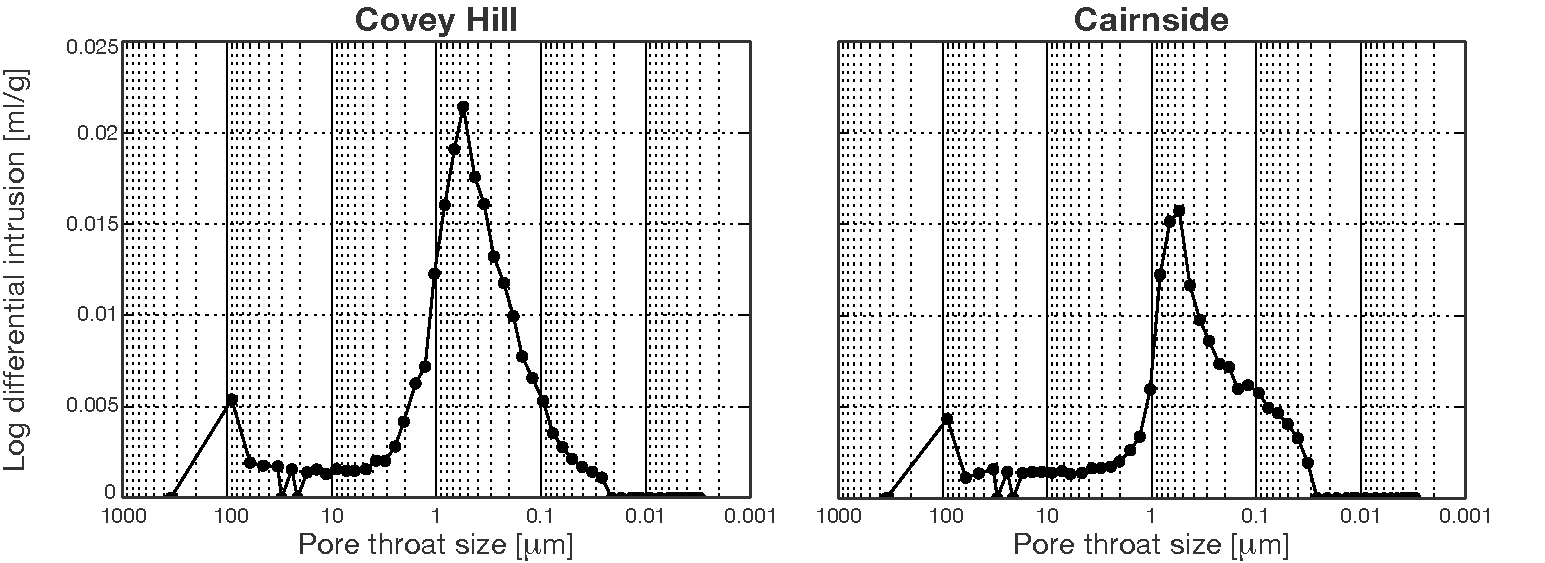
\includegraphics[width=1\textwidth]{fig/pore_size.pdf}
\caption{Log differential intrusion vs. pore size for the matrix of the Covey
Hill and Cairnside samples. Dominant pore throat sizes is
\SI{0.45}{\micro\metre} for both samples.}
\label{fig:poresize}
\end{figure}
\section{Time-lapse seismic response modeling}
Vertical seismic profile (VSP) methods are well suited for pilot carbon
sequestration projects as, on one hand, they provide higher vertical resolution
information than surface seismic \citep{Yang2014} while on the other they allow
for multiple economical repeat surveys. Indeed, VSP surveys for \ce{CO2}
monitoring have been used at pilot-scale \ce{CO2} injection sites such as Ketzin
\citep{Yang2010, Ivandic2012, Gotz2014, Diersch2014}, SACROC
\citep{Yang2014,Cheng2010}, Frio \citep{Daley2007}, and Otway
\citep{Urosevic2008}. VSP methods have been also used in commercial projects
such as IEA GHG Weyburn-Midale \ce{CO2} Monitoring and Storage Project
\citep{Bellefleur2004} and Aquistore \citep{White2014}.\\
 For this study, numerical simulation of time-laspe VSP surveys has been
conducted as preparatory work for a future VSP monitoring program.
\subsection{Methodology}
Seismic modeling is a technique for simulating wave propagation in the earth.
The objective is to predict a seismogram given a composition and structure of
the subsurface \citep{Carcione2010}. Seismic wave propagation can be modeled by
solving the wave equations for acoustic, elastic, viscoelastic, poroelastic or
poro-viscoelastic media. The procedure followed in this study to perform seismic
modeling is directly inspired by the work of \citet{Carcione2006} who present an
application of poro-viscoelastic modeling for monitoring underground \ce{CO2}
storage. The poro-viscoelastic formulation represents perhaps the most effective
tool to study the effect of the saturating fluid on the seismic response because
fluid properties are directly taken into account in the equations. It is thus
not necessary to rely on fluid substitution models to compute effective seismic
moduli, and it is expected that fluid substitution effects are mode accurately
described. The modeling code used in this work is described in
\citet{Giroux2012}.\\
The elastic coefficients characterizing the porous media introduced by
\citet{Biot1957} and reported in \citet{Carcione1998} are:\\
The $P$-wave modulus of the matrix ($E$)
\begin{equation}
E = K_{dry} + \dfrac{4}{3}G,
\end{equation}
The coupling modulus ($M$) between the solid and the fluid
\begin{equation}
M = \dfrac{K_{s}^{2}}{D-K_{dry}} ,
\end{equation}
where the diffusion fucntion D is defined as
\begin{equation}
D = K_s \big[1 + \phi(K_s K_{f}^{-1} -1)\big],
\end{equation}
The poroelastic coefficient ($\alpha$) of effective stress
\begin{equation}
 \alpha = 1 - \dfrac{K_{dry}}{K_s},
\end{equation}
where $K_{dry}$, $K_s$, $K_f$ are the bulk moduli of the drained matrix, the
solid and the fluid respectively; $\phi$ is the porosity, and $G$ is the shear
modulus of the matrix (both cases of drained and saturated).
 \citet{Carcione1998} presented an approach to introduce viscoelasticity into
Biot's poroelastic equations, in which matrix-fluid mechanisms are modeled by
generalizing the coupling modulus $M$ to a time dependent relaxation function
while the others elastic coefficients are independent of frequency. Detailed
information on the implementation of the equations of motion can be found in
\citet{Carcione1998} and \citet{Carcione1999}.
\subsection{Geological model}
We consider a 2D idealized geometry and physical model to describe the
sedimentary sequence of the St. Lawrence Lowlands. The geological model consists
of a tabular succession of six horizontal layers corresponding to the Lorraine
group, Utica shales, Trenton group, Beekmantown group, Cairnside formation,
Covey Hill formation and the Grenville basement. The grid size is \SI{2000 x
1500}{\metre} with a cell size is \SI{1 x 1}{\metre}, leading to a total of
\num{3} million cells. For each cell, \num{11} parameters
($K_{dry},K_s,K_f,\phi,G_s,\rho_s,\rho_f,\tau,\eta,\kappa,Q$ -
\Cref{tbl:modelpar}) characterize the medium.
A sequential Gaussian simulation (SGS) framework is used to modify the classical
geological blocky model in order to obtain a more realistic heterogeneous model.
First, for each layer, we compute the mean ($\mu$) and the standard deviation
($\sigma$) of the physical properties (mineralogical composition (V$_{clay}$,
V$_{calcite}$, V$_{quartz}$, V$_{dolomite}$), $V_p$, $V_s$, porosity($\phi$) and
density ($\rho$) derived from log data available in the studied region. The dry
laboratory measurements are used to obtain the dry-rock bulk modulus that is one
main component of the model. The distribution of the physical properties are
then obtained by simple kriging under Gaussian hypothesis and used for computing
the model parameters as the following:\\
the dry-rock bulk modulus ($K_{dry}$) is estimated using inverse Gassmann's
equation \citep{Hamilton1971,Carcione2007}:
\begin{equation}
K_{dry} = \dfrac{(\phi \dfrac{K_s}{K_f} + 1 - \phi)K_{sat} - K_s}{\phi
\dfrac{K_s}{K_f} + \dfrac{K_{sat}}{K_s} - 1 - \phi},
\end{equation}
where $K_{sat} = \rho V_{P}^{2} - (4/3)G$ is the saturated bulk modulus.\par
The bulk ($K_s$) and shear ($G_s$) moduli of the solid are estimated using
\cref{eq:Ks} and (\ref{eq:Gs}) - see \cref{tbl:mineralpost} for the mineralogic
composition.
Tortuosity ($\tau$) is estimated using \citep{Glover2009}:
\begin{equation}
\tau = \phi^{1-m},
\end{equation}
where $m$ is the cementation factor.
The brine properties are obtained by using the equations given in
\citet{Batzle1992}. The pressure and temperature dependent bulk modulus ($K_f$),
density ($\rho_f$) and viscosity ($\eta_f$) of the \ce{CO2} are determined from
the thermodynamic properties obtained from NIST’s online chemistry webBook
\citep{Lemmon2014}. Permeabilities ($\kappa$) are taken from
\citet{TranNgoc2014}. The velocity fields for the heterogeneous and for the
classical block models are shown in \cref{fig:mstochvsblock}.
\begin{table}[!h]
%\ra{1}
  \centering
  \caption{Mineral composition of the Potsdam group sandstones.}
\begin{tabular}{lS[table-number-alignment = center,table-format =
2.0]S[table-number-alignment = center,table-format = 2.0]}
\toprule
 & {Cairnside} & {Covey Hill}\\
  & {\small{(\si{\percent})}} & {\small{(\si{\percent})}}\\
\midrule
 Quartz   & 90 & 82 \\
 Smectite  & 6 & 12 \\
 Calcite  & 2 & 3 \\
Dolomite  & 2 & 2 \\
\bottomrule
\end{tabular}
\label{tbl:mineralpost}
\end{table}
% \afterpage{
\begin{landscape}
\begin{table}[p]
  \caption{Parameters defining the geological model}
  \label{tbl:modelpar}
  \sisetup{}
  \centering
	\begin{threeparttable}[b]
	\begin{tabular}{@{}l
	S[table-format = 2.2]
	S[table-format = 3.2]
	S[table-format = 1.3]
	S[table-format = 2.2]
	S[table-format = 2.2]
	S[table-format = 4.0]
	S[table-format = 4.0]
	S[table-format = 2.2]
	S[table-format = 1.2]
	S[table-format = 1.1e-2]
	S[table-format = 3.2]
	@{}}
\toprule

& \textbf{$K_{dry}\tnote{*}$} & \textbf{$K_s$}\tnote{*} & \textbf{$K_f$} &
\textbf{$\phi$}\tnote{*} & \textbf{$G_s$}\tnote{*} & \textbf{$\rho_s$}\tnote{*}
& \textbf{$\rho_f$} & \textbf{$\tau$}\tnote{*} & \textbf{$\eta$} &
\textbf{$\kappa$} & \textbf{$Q$}\tnote{*} \\
& \scriptsize{dry rock} & \scriptsize{bulk modulus} & \scriptsize{bulk modulus}
& \scriptsize{porosity} & \scriptsize{shear} &\scriptsize{density }
&\scriptsize{density } & \scriptsize{tortuosity}&\scriptsize{fluids }
&\scriptsize{permeability} &\scriptsize{seismic } \\
& \scriptsize{bulk modulus} & \scriptsize{of the grains} & \scriptsize{of the
fluids}  &  & \scriptsize{modulus} &\scriptsize{of the grains} &\scriptsize{of
the fluids} & & \scriptsize{viscosity}& &\scriptsize{quality factor} \\
& \footnotesize{(\si{\giga\pascal})} & \footnotesize{(\si{\giga\pascal})} &
\footnotesize{(\si{\giga\pascal})}  &  \footnotesize{(\si{\percent})}
&\footnotesize{(\si{\giga\pascal})} &\footnotesize{(\si{\kg\per\cubic\metre})} &
\footnotesize{(\si{\kg\per\cubic\metre})}& \footnotesize{(-)}&
\footnotesize{(cP)}& \footnotesize{(\si{\metre\squared})}&\footnotesize{(-)} \\
\midrule

\multirow{2}{*}{Lorraine} & 9.91 & 50.62 & 2.3 & 14 & 9.14 & 2621 & 1000 & 2.67
& 1 & 1.9e-19 & 110 \\
						  &  & &&&&&&&&\\
\multirow{2}{*}{Utica shales} & 22.15 & 76.80 & 2.3 & 4.7 & 17.97 & 2662 & 1000
& 5.70 & 1 &  1.9e-19 & 141 \\
							  & &&&&&&&&&\\
\multirow{2}{*}{Trenton} & 34.44 & 108.59 & 3.2 & 1.6 & 23.85 & 2711 & 1150 &
18.96 & 1.3 &  1.9e-16 & 168 \\
						 & &&&&&&&&&\\
\multirow{2}{*}{Beekmantown} & 25.37 & 80.66 & 3.072 & 1.9 & 26.58 & 2704 & 1120
& 18.89 & 1.1 & 1.5e-16 & 156 \\
							 & &&&&&&&&&\\
\multirow{2}{*}{Cairnside} & 18.70 & 62.76 & 3.55 & 3.55 & 19.36 & 2662 & 1190 &
19.65 & 1.28 & 1.2e-16 & 133 \\
						   & &&&&&&&&&\\
\multirow{2}{*}{Covey Hill} & 16.27 & 65.25 & 2.9 & 6.6 & 18.73 & 2664 & 1090 &
12.08 & 1 & 2.4e-16 & 136 \\
							& &&&&&&&&&\\
\multirow{2}{*}{Basement} & 37.82 & 119.28 & 3.4 & 1.6 & 32.25 & 2670 & 1200 & 1
& 1 & 1.0e-19 & 175 \\
						  & &&&&&&&&&\\
\bottomrule
\end{tabular}
\begin{tablenotes}
\item [*] Mean values representing parameters that have been simulated.
\end{tablenotes}
\end{threeparttable}
\end{table}
\end{landscape}
% }
\begin{figure}[!ht]
        \centering
        \begin{subfigure}[b]{1\textwidth}
                \caption{Heterogeneous realistic model.}
                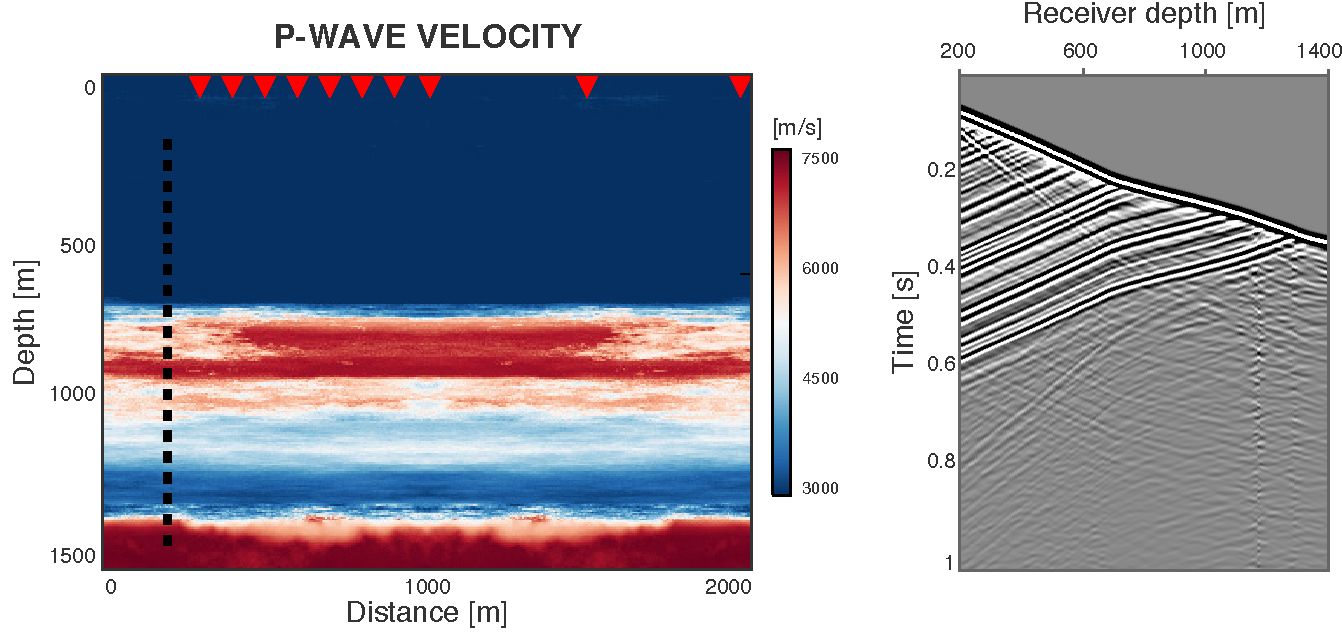
\includegraphics[width=\textwidth]{fig/model_stochvsblock_a.pdf}
                \label{fig:mstochvsblock_a}
        \end{subfigure}%

        \begin{subfigure}[b]{1\textwidth}
                \caption{Classical block model.}
                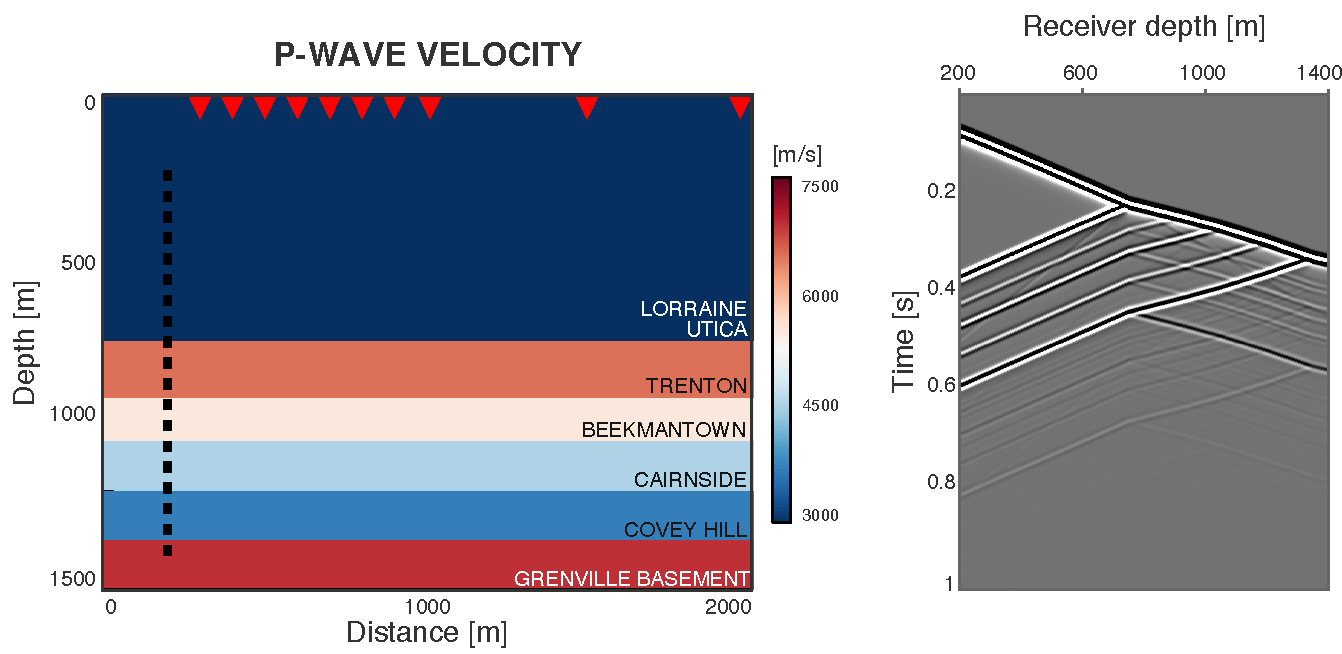
\includegraphics[width=\textwidth]{fig/model_stochvsblock_b.pdf}
                \label{fig:mstochvsblock_b}
        \end{subfigure}

        \caption{$P$-wave velocity for the heterogeneous and block model with
respectively seismograms.}
        \label{fig:mstochvsblock}
\end{figure}
\subsection{\texorpdfstring{\ce{CO2}}{CO2} injection modeling}
Modeling the seismic response to \ce{CO2} injection requires representative
models to correctly predict the system behavior. This implies fluid flow
modeling to predict the progression of \ce{CO2} plume in the reservoir. The
classic approach relies on three-dimensional numerical methods to solve the
system with a high degree of accuracy. However, this involves significant
computational efforts that are not always feasible. In recent years, approaches
that employ semi-analytical methods have been increasingly developed
\citep{Nordbotten2005a, Nordbotten2009}. One promising simulation tool for fast
and accurate modeling of \ce{CO2} sequestration is based on the vertical
equilibrium (VE) assumption. VE models have a long tradition for describing
flows in porous media; in hydrology it is known as the Dupuit approximation,
whereas in the oil industry is used to simulate two-phase and three phase
segregated flow \citep{Martin1958,Coats1967,Martin1968}. In recent years, VE
methods have been employed to simulate large scale \ce{CO2} injection and
migration, for which a sharp interface assumption with vertical equilibrium may
be reasonable due to the large density difference between supercritical \ce{CO2}
and brine \citep{Nordbotten2005a,Celia2006, Nordbotten2006}.\\
For the purpose of this study, we used the VE solvers included in the Matlab
Reservoir Simulation Toolbox (MRST) \citep{Lie2011}, to model the \ce{CO2}
injection, where the heterogeneous geological model built in the previous
section is used as input. Two different scenarios are proposed: an optimistic
scenario (\cref{fig:seismopt}), where  porosity and permeability reflect those
of the Ketzin pilot project \citep{Michael_2010}, and a Bé\-can\-cour-like
scenario (\cref{fig:seismbec}). The model simulates injection of \ce{CO2} in the
Potsdam formations during \num{15} years at an injection rate of
\SI{45}{\tonne\per\day}. This rate is comparable to the average rate for
injection at Ketzin \citep{Martens_2012}. This injected \ce{CO2} allowed to
migrate further outward for the next \num{35} years. The total storage of
\ce{CO2} is \SI{245}{\kilo\tonne}. The properties of the model are summarized in
\cref{tbl:co2par}. The \ce{CO2} plume for the Bé\-can\-cour-like scenario is
limited to a few hundreds of meters around the well due to its low
permeabilities and porosity. The results are consistent with those obtained by
\citet{TranNgoc2013} using TOUGH2 \citep{Pruess1999,Pruess2005}. For the
optimistic scenario (where permeabilities and porosities are respectively
\numlist{2000;2} times greater than the Bé\-can\-cour-like scenario), the plume
extends for more than a kilometer. During the migration time the \ce{CO2} is
partially dissolved for the latter scenario, while it is not the case in the
Bé\-can\-cour-like scenario.
\begin{figure}[!ht]
        \centering
        \begin{subfigure}[b]{0.95\textwidth}
                \caption{5 years monitoring}
                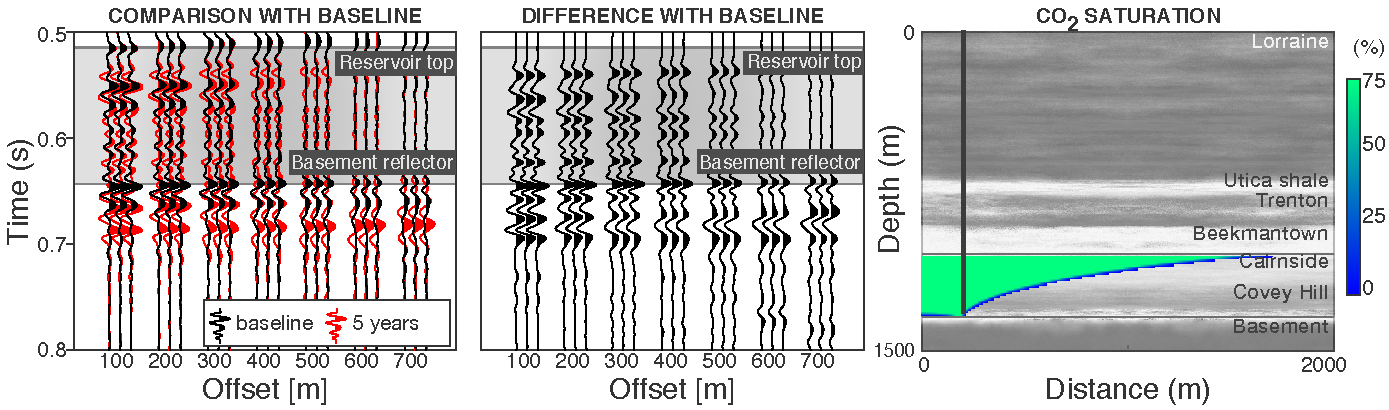
\includegraphics[width=\textwidth]{fig/seism_opt_new_a.pdf}
                \label{fig:seism_opt_a}
        \end{subfigure}%

        \begin{subfigure}[b]{.95\textwidth}
                \caption{15 years monitoring}
                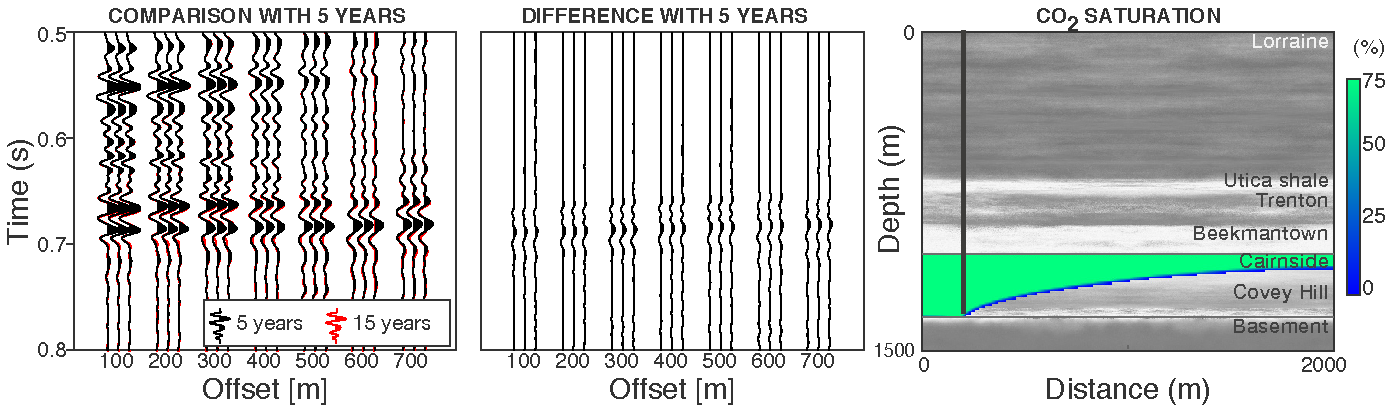
\includegraphics[width=\textwidth]{fig/seism_opt_new_b.pdf}
                \label{fig:seism_opt_b}
        \end{subfigure}

        \begin{subfigure}[b]{.95\textwidth}
                \caption{50 years monitoring}
                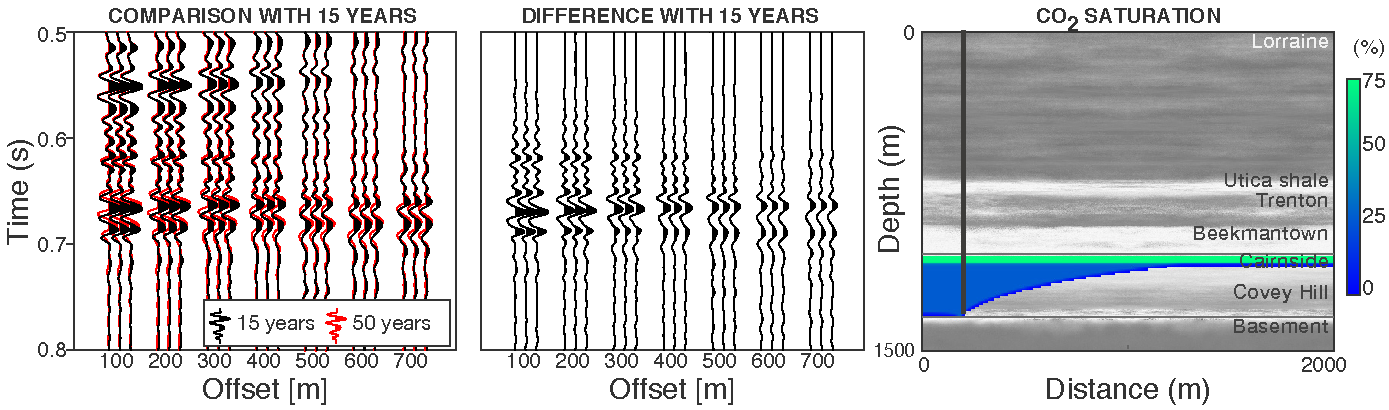
\includegraphics[width=\textwidth]{fig/seism_opt_new_c.pdf}
                \label{fig:seism_opt_c}
        \end{subfigure}

        \caption{Corridor stack difference (3 traces for each offset) for the
optimistic scenario.}
        \label{fig:seismopt}
\end{figure}

\begin{figure}[!ht]
        \centering
        \begin{subfigure}[b]{0.95\textwidth}
                \caption{5 years monitoring}
                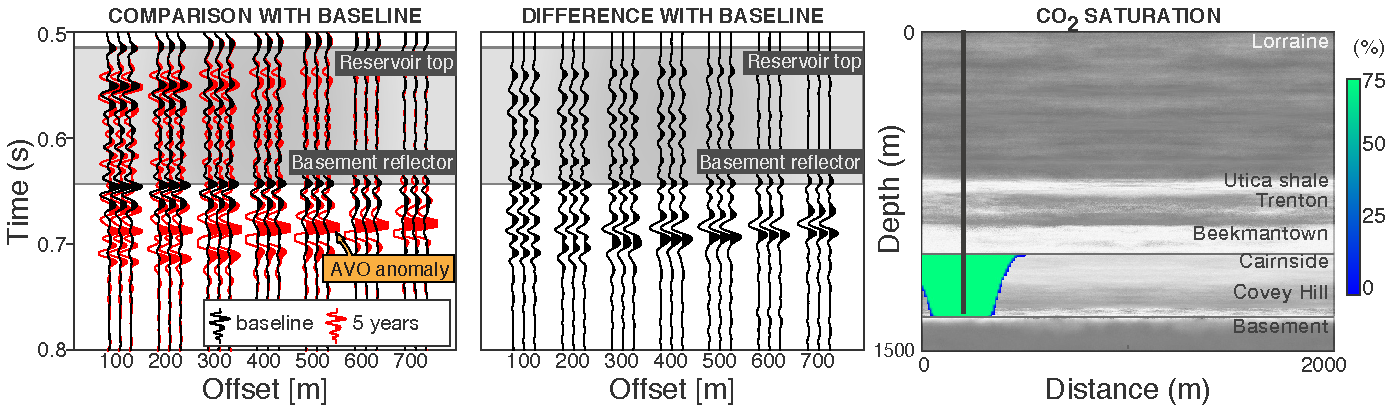
\includegraphics[width=\textwidth]{fig/seism_bec_new_a.pdf}
                \label{fig:seism_bec_a}
        \end{subfigure}%

        \begin{subfigure}[b]{.95\textwidth}
                \caption{15 years monitoring}
                \includegraphics[width=\textwidth]{fig/seism_bec_new_b.pdf}
                \label{fig:seism_bec_b}
        \end{subfigure}

        \begin{subfigure}[b]{.95\textwidth}
                \caption{50 years monitoring}
                \includegraphics[width=\textwidth]{fig/seism_bec_new_c.pdf}
                \label{fig:seism_bec_c}
        \end{subfigure}

        \caption{Corridor stack difference (3 traces for each offset) for the
B\'e\-can\-cour like scenario.}
        \label{fig:seismbec}
\end{figure}
\begin{table}
  \centering
  \caption{Models parameters for the \ce{CO2} injection simulation and for
synthetics seismograms}
 \begin{tabular}{p{3.5cm}lSS}
\toprule
  && {\textbf{Bé\-can\-cour-like}} & {\textbf{Optimistic}}   \\
\cmidrule(r){3-4}
Avg. porosity at reservoir &(\si{\percent})  &  6  &  20   \\
Avg. permeability & (\si{\metre\squared})  & 3.06e-16  & 6.5e-13  \\
x range &(\si{\metre}) & \multicolumn{2}{c}{2000 }  \\
z range &(\si{\metre}) & \multicolumn{2}{c}{1500 }  \\
Injection depth &(\si{\metre}) & \multicolumn{2}{c}{1200-1350 }  \\
Injection rate &(\si{\tonne\per\metre}) & \multicolumn{2}{c}{45 }  \\
Injection time &(years) & \multicolumn{2}{c}{15 }  \\
Migration time &(years) & \multicolumn{2}{c}{35}  \\
Total storage &(\si{\kilo\tonne}) & \multicolumn{2}{c}{245}\\
Source offsets &(\si{\metre}) & \multicolumn{2}{c}{100, 200, 300, 400, 500, 600,
700}    \\
Receiver x coordinate &(\si{\metre}) & \multicolumn{2}{c}{200} \\
Receiver z coordinate &(\si{\metre}) & \multicolumn{2}{c}{200-1400} \\
Receiver spacing &(\si{\metre}) & \multicolumn{2}{c}{5} \\
Total traces & & \multicolumn{2}{c}{241} \\
\bottomrule
\end{tabular}
\label{tbl:co2par}
\end{table}
\subsection{Synthetic seismograms}
The aim of the modeling exercise is to simulate time-lapse VSP surveys. We are
interested in analyzing what is the effect of the injected \ce{CO2} after
\numlist{5;15;50} years from the start of injection as shown in
\cref{fig:seismopt,,fig:seismbec}. Large (\SI{>700}{\metre}) amplitude versus
offset analysis (AVO) \citep{Backus1982,Ostrander1982,Ostrander1984} in our work
are compromised due to a refracted wave (\cref{fig:refracted}) that arises at
the interface between the Lorraine/Utica shales and Trenton group, preventing a
proper separation of upgoing and downgoing waves. The parameters for the
synthetic seismograms are summarized in \cref{tbl:co2par}.
% \begin{figure}[!ht]
% \centering
% \includegraphics[width=0.8\textwidth]{fig/refracted_new.pdf}
% \caption{Refracted wave that arise at large offset (\SI{>700}{\metre}). a)
% Snapshot of the wave propagation at 300 ms and b) resulting seismogram.}
% \label{fig:refracted}
% \end{figure}
\begin{figure}[!ht]
        \centering
        \begin{subfigure}[b]{0.75\textwidth}
                \caption{Snapshot of the wave propagation at 300 ms for source
placed at \SI{2000}{\metre}.}
                \includegraphics[width=1\textwidth]{fig/refracted_new_a.pdf}
                \label{fig:refracted_a}
        \end{subfigure}%

        \begin{subfigure}[b]{0.75\textwidth}
                \caption{Resulting seismogram.}
                \includegraphics[width=1\textwidth]{fig/refracted_new_b.pdf}
                \label{fig:refracted_b}
        \end{subfigure}

        \caption{Refracted wave that arise at large offset (\SI{>700}{\metre}).}
        \label{fig:refracted}
\end{figure}


\begin{table}
%\ra{1}
  \centering
  \caption{Synthetic seismogram processing}
\begin{tabular}{@{}cl@{}}
\toprule
 \textbf{Step} & \textbf{Processing operation}\\
\midrule
1   & Trace edit \\
2  & Pick first arrival  \\
3 & Velocity analysis on the zero offset shot\\
4  & f-k filter to separate upgoing and downgoing waves \\
5 & NMO analysis\\
6 & Static: flatten the upgoing wave using the first arrivals  \\
7 & VSP corridor mute\\
8 & VSP stack (3 traces)\\
 \bottomrule
\end{tabular}
\label{tbl:process}
\end{table}
\subsection{Modeling results}
In this section we present the results of three synthetic seismograms, for 5, 15
and 50 years after the start of CO$_2$ injection, for both B\'ecancour and
optimistic scenarios (\cref{fig:seismbec,fig:seismopt} respectively).
% \Cref{fig:seism_opt_a,fig:seism_bec_a} show the results for 5 years
% monitoring; \cref{fig:seism_opt_b,fig:seism_bec_b} show the results for 15 year
% monitoring and \cref{fig:seism_opt_c,fig:seism_bec_c} show the results for 50
% year monitoring.
The processing has been inspired by the work of \citet{Coulombe1996,Zhang2010};
the main steps are summarized on \cref{tbl:process}.
\subsubsection{Optimistic scenario}
\Cref{fig:seismopt} shows the corridor stack (\num{7} offsets) for the
optimistic scenario. \Cref{fig:seism_opt_a} shows the comparison and the
difference between baseline and \num{5} years monitoring. The effect of \ce{CO2}
 is mainly observed by a travel-time delay starting at \SI{550}{\ms}. Other
authors reported similar observations \citep{Yang2014,Arts2004}. The delay is
evaluated by crosscorrelation between baseline and 5 years timelapse for each
offset and is of about 30 ms as showed in \cref{tbl:delay}.
\Cref{fig:seism_opt_b} shows the comparison and the difference between
\numlist{5,15} years monitoring. The differences detected are minimal. This is
confirmed by the shape of the \ce{CO2}  plume that after \num{15} years of
injections has the same shape than after \num{5} years. \Cref{fig:seism_opt_c}
shows the comparison and the difference between \numlist{15,50} years
monitoring. The \ce{CO2}  injection modeling show that during migration time
(\numrange{15}{50} years) there is partial dissolution of \ce{CO2} . This is
reflected in the \num{50} years (red traces), with reflections that arrive
\SI{5}{\ms} earlier when compared to the \num{15} years (black traces).
\begin{table}[!bh]
%\ra{1}
  \centering
  \caption{Signal delay between the baseline survey and seismic traces collected
5 years after the CO2 injection.}
\begin{tabular}{@{}cc@{}}
\toprule
  Offset (m) & Delay (ms)\\
  % & \small{[\%]} & \small{[\%]}\\
\midrule
 100   & 22.50  \\
 200   & 23.00  \\
 300   & 33.75  \\
 400   & 33.00  \\
 500   & 31.50  \\
 600   & 30.75  \\
 700   & 30.25  \\
 \textbf{mean}  & \textbf{29.25}  \\
\bottomrule
\end{tabular}
\label{tbl:delay}
\end{table}
\subsubsection{Bécancour scenario}
\Cref{fig:seismbec} shows the corridor stack (7 offsets) for the Bécancour
scenario. \Cref{fig:seism_bec_a} shows the comparison and the difference between
baseline and \num{5} years monitoring. As for the optimistic scenario, the
effect of \ce{CO2} is mainly observed by a travel-time delay starting at
\SI{550}{\ms}. \Cref{fig:seism_bec_b} shows the comparison and the difference
between \numlist{5,15} years monitoring. The differences are highlighted at
\SI{700}{\ms} due to the greater extension of the \ce{CO2} plume compared to the
\num{5} years monitoring. \Cref{fig:seism_bec_c} shows the comparison and the
difference between \num{15} years and \num{50} years monitoring. The difference
highlighted at \SI{700}{\ms} are minimal and mostly caused by the lower \ce{CO2}
saturation, due to the partial dissolution of \ce{CO2} during the migration
time.
An AVO anomaly with an amplitude increase with the offset at the basement
reflection is also evident.\\
\Cref{fig:stochvsblock} shows the comparison of the seismograms obtained from
the heterogeneous geological model (left) versus a blocky model (right) for a
\num{5} years time-lapse. As expected, the lack of complex details in the blocky
model is reflected in the seismograms. For example, the time-delay at
\SI{550}{\ms} is not observable in the blocky seismogram and the \ce{CO2} effect
is only detected by an amplitude variation.\\
% \begin{figure}[!ht]
% \centering
% \includegraphics[width=0.9\textwidth]{fig/stochvsblock.pdf}
% \caption{Stochastic seismogram (left) versus block seismogram (right).}
% \label{fig:stochvsblock}
% \end{figure}
\begin{figure}[!ht]
        \centering
        \begin{subfigure}[b]{.5\textwidth}
                \caption{Heterogeneous model \\ (after 5 years)}
                \includegraphics[width=\textwidth]{fig/stochvsblock_a.pdf}
                \label{fig:stochvsblock_a}
        \end{subfigure}%
        \begin{subfigure}[b]{.5\textwidth}
                \caption{Block model \\ (after 5 years)}
                \includegraphics[width=\textwidth]{fig/stochvsblock_b.pdf}
                \label{fig:stochvsblock_b}
        \end{subfigure}
        \caption{Seismogram based on the heterogeneous model and blocky model}
        \label{fig:stochvsblock}
\end{figure}
Moreover, at the Potsdam bottom reflector, the blocky model shows an amplitude
decrease with offset. However, for the heterogeneous model, the same reflection
shows an increasing amplitude with offset. This is confirmed by the Zœppritz
analysis \citep{Aki1980} in \cref{fig:zoeppritz} where the reflection
coefficients change with the angle of incidence.
\begin{figure}[!ht]
\centering
\includegraphics[width=1\textwidth]{fig/zoeppritz.pdf}
\caption{Zœppritz analysis for heterogeneous model (a) and blocky model (b)
using the CREWES Zœppritz Explorer Applet. The graphs on the right show how
reflection coefficient change with angle of incidence.}
\label{fig:zoeppritz}
\end{figure}
\section{Conclusion}
Ultrasonic measurements have been carried out on Cairnside and Covey Hill
samples of the sedimentary basin of the St.\ Lawrence Platform in southern
Quebec. The results show that $P$-waves are sensitive to pore fluid substitution
at the laboratory scale. Moreover, the measurements demonstrate that it is
possible to detect the phase transition from gaseous \ce{CO2} to liquid or
supercritical \ce{CO2}, for both velocity and amplitude attributes. \\
The laboratory measurements were used for calibrating numerical models that were
used to simulate the time-lapse seismic response to \ce{CO2} injection. A number
of scenarios were considered to evaluate the performance of a time-lapse seismic
monitoring program for the particular context of the St.\ Lawrence Platform. We
were particularly interested in comparing the response of a blocky model
(commonly used in comparable studies) with that of a model reflecting the
natural variability found in nature. We were also interested in assessing the
effect of the low permeability and porosity observed at Bécancour on the
time-lapse seismic response, and comparing the performance the seismic
monitoring with respect to more favorable storage conditions.\\
For all scenarios, a series of VSP synthetic seismograms imaging the \ce{CO2}
evolution during \num{15} years of injection and the subsequent \num{35} years
of \ce{CO2} migration have been modeled. The results show the effect of \ce{CO2}
as indicated by a time-delay of arrivals, associated with a decrease in velocity
when supercritical \ce{CO2} replaces brine in pore spaces. The geostatistical
approach used to generate our heterogeneous model allowed us to obtain more
realistic seismograms compared to a traditional blocky model. The time-lapse
amplitude response of the blocky and heterogeneous models also differ
significantly in the lower part of the reservoir.  Using over simplistic models
thus yields misleading results. It should be noted nevertheless that the
conclusions regarding the capabilities of the VSP monitoring program, as
obtained with the heterogeneous model, might be somewhat optimistic because
repeatability issues inherent to field measurements might affect its
performance.\\
For the Bécancour model, there is almost no evolution of the \ce{CO2} plume
after \num{5} years of injection and even \num{35} years after injection
stopped, and it is therefore unlikely to detect any long-term variation in the
seismic response. However, in the optimistic case the \ce{CO2} has been
partially dissolved during the migration period, and the VSP response after 50
years results in an early arrival of the reservoir bottom signal compared to the
15 years data. Therefore, carefully considering the behaviour of the reservoir
in modeling the seismic response appears critical for accurate appraisal of the
time-lapse response, which will help interpreting correctly real monitoring
data. \\
These results highlight the fact that details in the models can have significant
impacts on the expected response to a monitoring campaign. One element that was
not considered in this work are the changes in wave speeds resulting from
varying pore pressures during the injection of \ce{CO2} in the reservoir. As
reported in the literature and reiterated in the new measurements described in
this contribution, pressure effects can affect the seismic response and change
the results modeled in this study (see review in \citet{Schmitt2015}). In
particular, as pressure redistributes over time, the long-term seismic response
modeled in the Bécancour scenario should also change over time, contrary to what
is predicted without considering pressure change in the simulations.  Work is
under way to take such effects into account.
\section{Acknowledgements}
The authors would like to acknowledge E. Gloaguen for constructive comments on
an early version of the manuscript. Financial support was provided by the INRS
research chair on carbon dioxide geological storage granted by the Minist\`ere
du D\'e\-ve\-loppe\-ment durable, de l'En\-vi\-ron\-ne\-ment et des Parcs of
Qu\'ebec, as well as a research grant from Carbon Management Canada.
Computational resources were supplied by Calcul Quebec and Compute Canada.
Zœppritz analysis has been made with the Zœppritz explorer tool developed by the
Consortium for Research in Elastic Wave Exploration Seismology (CREWES).

% \end{spacing}
\renewcommand{\bibname}{Références}
\addcontentsline{toc}{chapter}{\bibname}
\begin{singlespacing}
\putbib[biblio/biblio]
\end{singlespacing}
\end{bibunit}

\renewcommand{\chaptername}{Article}
\begin{bibunit}[bibliostyleINRS]
% \begin{spacing}{1.5}
%!TeX root = Thesis_LP.tex
% \sisetup{
% list-final-separator= { and },    % Place "et" à la fin de la liste
% range-phrase= { to }             % Place "à" à entre la gamm
% }

\pagestyle{fancy}
\fancyhf{}
\renewcommand{\headrulewidth}{0pt}
\fancyhead[LO]{\emph{Article 2. Stochastic \ce{CO2} monitoring}}
\fancyhead[RO]{\thepage}
\fancyhead[LE]{\thepage}


\chapter{Stochastic inversion workflow using the gradual deformation to estimate
reservoir properties and predict the \texorpdfstring{\ce{CO2}}{CO2} distribution
within a saline aquifer}
\label{ch:article2}
\selectlanguage{english}

\chaptermark{Stochastic \ce{CO2} monitoring} % Titre court apparaissant dans
% l'entête des pages

{\setlength{\parindent}{0cm}
\underline{\textbf{Titre traduit}}\\
Flux de travail d'inversion stochastique utilisant la déformation graduelle
pour estimer les propriétés de réservoir afin de prédire la distribution du
\ce{CO2} dans un aquifère salin.

\underline{\textbf{Auteurs}}\\
Lorenzo Perozzi$^1$, Erwan Gloaguen$^1$, Bernard Giroux$^1$\\
$^1$ Institut national de la recherche scientifique - Centre Eau Terre
Environnement, 490, de la Couronne, Qu\'ebec, QC, G1K 9A9, CANADA

\newpage
\underline{\textbf{Contribution}}
{\setstretch{1.0}
\begin{description}[leftmargin=!,labelwidth=\widthof{\bfseries Erwan Gloaguen}]
  \setlength\itemsep{0.7em}
  \item[Lorenzo Perozzi] Conceptualisé et réalisé (les mesures de laboratoire,
la modélisation sismique, l’interprétation des résultats) l’étude et rédigé
l’article
  \item[Erwan Gloaguen]  Conceptualisé l'étude, fourni des conseils sur
l’interprétation des résultats et contribué à la rédaction de l’article.
  \item[Bernard Giroux]  Contribué à la rédaction de l’article. \\
\end{description}
}

\underline{\textbf{Publication ciblée}}\\
{\setstretch{0.5}
Computational Geosciences\\
à soumettre\\
}

\underline{\textbf{Résumé traduit}}\\
En raison de contraintes financières, la séquestration géologique du \ce{CO2}
dans les aquifères salins est souvent effectuée en utilisant uniquement un puits
injecteur et un puits de surveillance, ce qui limite sérieusement la
compréhension de la dynamique du panache de \ce{CO2}. Dans ce cas, la
surveillance du \ce{CO2} repose uniquement sur des hypothèses géologiques ou sur
les données indirectes. Dans ce travail, on présente une nouvelle approche en
deux étapes pour l'inversion des ondes $P$ et $S$, de la densité et de la
porosité permettant une prédiction fiable
de la distribution du \ce{CO2}. Dans la première étape, on calcule plusieurs
ensembles de modèles stochastiques des propriétés élastiques en utilisant des
cosimulations séquentielles gaussiennes. Les réalisations de chaque ensemble
sont ensuite combinées entre elles de façon itérative en utilisant une technique
d'optimisation par déformation graduelle où la différence entre les traces
sismiques calculées et observées devient la fonction objectif. Dans la deuxième
étape, les résultats obtenus de l'étape précédente constituent les modèles
d'entrée pour le calage historique, toujours par déformation graduelle, de
l'injection du \ce{CO2}. À chaque itération, on simule l'écoulement du \ce{CO2}
et on calcule les traces sismiques correspondantes qui sont comparées aux traces
observées. Ce flux de travail a été testé sur un modèle hétérogène qui reproduit
l'environnement que l'on retrouve dans la région de Bécancour au Québec. Les
résultats montrent que les modèles optimisés ont une plus grande similarité
structurale avec les modèles de référence, comparée aux simulations
conventionnelles.
}

\section{Abstract}
Due to budget constraints, CCS in deep saline aquifers is often carried out
using only one injector well and one control well, which seriously limits
the understanding of the \ce{CO2} plume dynamics. In such case, monitoring of the
plume of \ce{CO2} only relies on geological assumptions or indirect data. In this
paper, we present a new two-step stochastic $P$- and $S$-waves, density and
porosity inversion approach that allows reliable monitoring of \ce{CO2} plume
using time-lapse VSPs. In the first step, we compute several sets of stochastic
models of the elastic properties using conventional sequential Gaussian
cosimulations. Each realization within a set of static models are then
iteratively combined together using a modified gradual deformation optimization
technique with the difference between computed and observed raw traces as
objective function. In the second step, these statics models serve as input for
a \ce{CO2} injection history matching using the same modified gradual
deformation scheme. At each gradual deformation step the \ce{CO2} injection is
simulated and the corresponding full-wave traces are computed and compared with
the observed data. The method has been tested on a synthetic heterogeneous
saline aquifer model mimicking the geological environment of the
Becancour area, Quebec. The results show that the set of optimized models of
$P$- and $S$-waves, density and porosity showed an improved structural similarity
with the reference models compared to conventional simulations.
\section{Introduction}
One of the major challenges limiting large-scale deployment of Carbon Capture
and Storage (CCS) operations is the issue of evaluating and forecasting the fate
of \ce{CO2} in deep rock formations. The characteristics of the reservoir
determined from the very beginning the design and operational conditions of most
of the CCS chain.  Indeed, having a comprehensive knowledge of the physical
characteristics of the storage site is crucial to determine the optimal rate of
\ce{CO2} injection, which influences the rate of capture, as well as the
parameters of a proper monitoring strategy.  Let us recall that monitoring is an
essential component of any CCS project and that most, if not all, jurisdictions
require more or less elaborated monitoring, verification and accounting (MVA)
programs (e.g.\ European CCS directive \citep{EU2014}).\\
A common task in CCS projects is thus to monitor the spatial distribution of
\ce{CO2} over time. However, the spatial distribution of the \ce{CO2} plume that
is estimated through monitoring is often inconsistent, to varying degrees, with
model-based simulations \citep{Ramirez2013}. This is mainly due to the lack or
sparseness of direct measurements of the reservoir petrophysical properties,
the low spatial coverage of geophysical surveys,  the underlying resolution of
inversion techniques and to uncertainties that limits the understanding of the
subsurface and therefore the ability to produce accurate reservoir models
allowing reliable forecasts of the \ce{CO2} plume.\\
The process of optimizing a reservoir model to fit dynamic data is commonly
known as history matching and is extensively used in the oil and gas industry \citep{Roggero1998}.
In conventional history matching, the target variables are reservoir engineering
properties such as pressure, water-cut, rate of production of oil, and the like,
all involving at least one injector and one pumping well. In \ce{CO2} storage
projects, such well configuration is not conceivable (pumping is not done) and
only one injector well is usually available. In this context, only indirect data
have the spatial coverage and the potential to improve the estimation of the
\ce{CO2} plume within the deep saline aquifers.\\
History matching requires the knowledge, at least in the stochastic sense, of
the spatial distribution of the static properties of the reservoir (porosity,
permeability). Due to the geological complexity and the scarcity of direct
observations (i.e.\ well data), probabilistic methods appear to be the most
suitable choice to build a reliable reservoir model. In addition, it is
established that seismic measurements are well suited to constrain static
reservoir properties modeling as they provide indirect but correlated and
spatially extensive information about reservoir properties \citep{Doyen2007}.\
The estimation of static parameters from seismic data is a complex,
ill-conditioned, nonlinear inverse problem due principally to the limited
bandwidth  of the seismic data, noise, measurement errors,
and  the assumptions underlying to forward models \citep{Tarantola2004}.
Seismic inverse problems may be developed following deterministic or
probabilistic approaches and can be divided into two main categories: (1)
multiple step inversion methods and (2) stochastic inversion methods
\citep{Grana2012}.\\
In multiple step inversion methods, the problem of estimating reservoir
properties from seismic data is split into two or more subproblems; elastic
properties are first derived from partial stacked seismic data through elastic
inversion; then, reservoir properties are classified by statistical techniques,
such as Bayesian classification \citep{Avseth2001,Mukerji2001,Buland2003}.\\
Iterative stochastic inversion methodologies solve the seismic inverse problem
using deterministic or stochastic optimization techniques. First, a set of
equivalent earth models is simulated using a stochastic algorithm based on prior
information usually from available well log data and a spatial continuity
pattern (e.g.\ variogram, training image) to create fine-scale reservoir models
\citep{Bosch2009}. Then suitable rock-physics transforms are applied to generate
the corresponding volumes of the elastic properties. Finally, synthetic seismic
volumes are computed and compared to real seismic data to evaluate the mismatch.
Several optimization methods exist to infer the elastic properties based on the
measured traces. \citet{Gonzalez2008} performed a trace-by-trace deterministic
optimization, \citet{Bosch2009} proposed an iterative optimization based on
Newton's method; Markov chain Monte Carlo approach has been used successfully
for the stochastic exploration of the model space
\citep{Eidsvik2004,Larsen2006,Gunning2007,Rimstad2010,Ulvmoen2010,Hansen2012}.
\citet{Grana2012} show the efficiency of the probability perturbation method
\citep{Caers2006} to estimate fine-scale reservoir models in a stochastic
inversion. A multidimensional scaling technique was successfully applied by
\citet{Azevedo2013} to asses how the parameter model space is explored by global
elastic inversion algorithm.
In addition to the static information and in order to evaluate the performance
of the reservoir in terms of \ce{CO2} storage, reservoirs models need to be
constrained by dynamic data obtained from the \ce{CO2} injection operations. To
be meaningful, reservoir models must match the observed dynamic behavior of the
reservoir within some interval of tolerance. History matching is also an
ill-posed problem and can be solved using the same algorithms as the one used
for estimating the static properties, but then involving the injection data and
forward fluid flow modeling.
In this paper we propose a stochastic inversion workflow using a modified
gradual deformation parametrization method \citep{Roggero1998} as a stochastic
optimization technique that integrates geophysical and geological logs, seismic
reflection data and \ce{CO2} flow simulations in order to analyze and monitor
the \ce{CO2} injection and its propagation within a saline aquifer.  This paper
is organized as follows. In the first section, we focus on each step of the
seismic inversion algorithm. The second section presents an the application of
the approach to characterize a synthetic reservoir for the \ce{CO2} injection in
the St.\ Lawrence Lowlands, Quebec, Canada.
\section{Methodology}
\label{sc:metho_art2}
The flowchart of the stochastic inversion that we propose is shown in
\cref{fig:workflow}.  It is a three step approach. Firstly, many sets of initial
realizations are simulated from available static data (well logs, deterministic
elastic inversion, etc.) using a geostatistical cosimulation algorithm.
Secondly, an optimization loop is applied to each set before modeling \ce{CO2}
injection in order to obtain a static model of petrophysical properties that
maximize the match between computed and observed seismic traces. Finally, the
resulting models are then combined in an iterative history-matching loop where,
at each step, we simulate \ce{CO2} injection and transport, compute the elastic
properties of the corresponding model, and run a seismic forward model to
calculate the mismatch between simulated and observed traces. In the following
sections, we focus on each step of the algorithm.
\begin{figure}[!ht]
\centering
\includegraphics[width=0.68\textwidth]{fig/workflow_authorea.pdf}
\caption{Workflow of the stochastic inversion methodology}
\label{fig:workflow}
\end{figure}
\subsection{Geostatistical methods}
In our approach, $P$ and $S$-wave velocity ($V_p$ and $V_s$), porosity ($\phi$)
and density ($\rho$) are first simulated using Sequential Gaussian CoSimulation
(SGCS) \citep{Deutsch1998,Doyen2007}. SGCS is a method that allows simulating
continuous random variables and that requires only the knowledge of their
variogram, histogram and coefficient of correlation. Starting from prior
information available form well log data, the algorithm visits each node of the
grid along a random path. At each step along this path, the algorithm
co-simulates a series of values for each variable. At each node, the prior
information and the previously simulated values are used to compute the kriging
mean and variance of each variable. This feedback loop ensures that the
simulation is spatially correlated. By construction, SGCS  will be conditioned
to the well data, i.e.\ the simulations reproduce the well observations and thus
have the same overall statistical properties. Multiple simulation are generated
by using different random paths and random seeds in order to obtain independent
sets of realizations. For an extended review about SGCS methods, refer to
\citet{Deutsch1998} and \citet{Doyen2007}.
\subsection{Static optimization}
In the second step of the algorithm, realizations of each set are iteratively
combined using the gradual deformation (GD) method \citep{Hu2000} as a
optimization technique. The GD is a parametrization method that allow to
iteratively perturb a set of realizations until obtaining a new realization that
minimizes the mismatch with some observed data. This method was first developed
for history matching purposes \citep{Roggero1998} and involves the linear
combination of Gaussian random fields with weights that are adjusted to minimize
the data mismatch while preserving the spatial covariance. Many variations of
this technique have since been presented
\citep{Roggero1998,Hu2000,Hu2002,Hu2001,LeRavalec2000,LeRavalec2012}. The key
idea behind the GD is that the sum of two Gaussian random field ($Y1$ and $Y2$)
is also a Gaussian random field:
\begin{equation}
Y(r) = Y_1\ cos(r) + Y_2\ sin(r)
\end{equation}
where $r$ are the gradual deformation coefficient. It can be shown that $Y(r)$
is a realization with the same mean and covariance as $Y_1$ and $Y_2$ whatever
the value of the deformation parameter $r$. This primary gradual combination
scheme involves independent realizations only, meaning that the $Y_1$ and $Y_2$
realizations are unconditional. To combine conditional realization, a variant of
the GD named gradual conditioning (GC) method was developed by \citet{Ying2000}
and \citet{Hu2002}. In this case, the  weights have to satisfy a new constraint.
Their sum has to be one while their sum to the square is also one. Within this
conditions, the realization built from two conditional realizations is also
conditional to the measured data and reproduce the overall covariance.
\citet{Hu2002} proposes the weights parametrization as follows:
\begin{equation}
\begin{cases}
    \alpha_1 = \dfrac{1}{3} + \dfrac{2}{3}\ cos(r)\\
    \alpha_2 = \dfrac{1}{3} + \dfrac{2}{3}\ sin\bigg(-\dfrac{\pi}{6}+r\bigg)\\
    \alpha_3 = \dfrac{1}{3} + \dfrac{2}{3}\ sin\bigg(-\dfrac{\pi}{6}-r\bigg)
    \end{cases}
\end{equation}
with parameter $r \in [-\pi,\pi]$. In comparison with the combination of
independent realizations, the above procedure avoids the conditioning step
during the optimization process.\\

When the GC method is incorporated into the optimization processes, the
deformation parameter $r$ becomes the parameter to adjust to reduce the
objective function.  At this stage, for each combination (i.e.\ for each value
of $r$) we obtain a new $V_p$, $V_s$ $\rho$ and $\phi$ field model. Afterwards,
the full-wave synthetic seismic response of the earth models $d_{synth}$ is
computed using an elastic finite-difference time-domain approach
\citep{Bohlen2002} and compared to the observed data $d_{obs}$. For this study,
the objective function is defined as the root mean square error between
$d_{obs}$ and $d_{synth}$:
\begin{equation}
J(r) = \sqrt{\frac{1}{N}\sum\limits_{i=1,N}\big(d_{synth}(r)-d_{obs}\big)^2}
\end{equation}
where $N$ is the number of the samples per trace and $i$ the sample index.
The combination for which $r$ minimize the mismatch between synthetic and
observed data is retained and combined with two initial SGCS realizations.
Ultimately, we obtain $V_p$, $V_s$, $\rho$ and $\phi$ fields that have the best
seismic match with the observed data.
\subsection{Dynamic optimization}
The results obtained after the previous step honor the static well-log data and
the variograms inferred from these data and the deterministic static inversion.
The aim now is to make the reservoir model consistent with the dynamic data
(i.e.\ \ce{CO2} injection and propagation within the reservoir). An iterative
history matching loop is started in which each iteration consists of the
following steps:
\begin{enumerate}
	\item run a fluid flow simulation;
	\item apply suitable rock-physics mapping to generate the corresponding volumes
of the elastic properties after \ce{CO2} injection;
	\item compute the seismic response;
	\item calculate the mismatch between simulated and observed data;
	\item perturb the model to lower the mismatch using gradual deformation.
\end{enumerate}
\subsubsection{Flow simulation}
In recent years, vertical-equilibrium (VE) models have been extensively used to
study gravity-driven \ce{CO2} migration \citep{Nordbotten2011}. Using an
analytical description for the vertical fluid distribution not only reduces the
dimensions of the problem but also lessens the coupling and increases the time
constants of the dynamic model \citep{Nilsen2014}. VE models are attractive
means to increase resolution while reducing computational burden, and are thus
particularly attractive for an iterative history-match loop where many flow
simulation steps are required. For the purpose of this study, we used the VE
solvers included in the Matlab Reservoir Simulation Toolbox (MRST)
\citep{Lie2012}, to model injection of CO$_2$ in the saline aquifer.
\subsubsection{Elastic properties}
\label{sc:elasticproperties}
Elastic properties are usually computed through a rock-physics model. This model
is a set of equations that transform petrophysical variables, typically
porosity, mineralogy and fluid saturations, into elastic properties such as $P$-
and $S$-wave velocity and density. For the purpose of this work, we first
estimate the elastic properties of the solid phase, i.e.\ bulk ($K_s$) and shear
($G_s$) moduli, by applying the arithmetic average of the upper and lower
Hashin-Shtrikman bounds \citep{Hashin1963}. Then we compute the elastic
properties of the fluid phase, i.e.\ bulk ($K_f$) modulus and density
($\rho_f$), using fluid mixing laws \citep{Wood1955,Brie1995}. \\
The new \ce{CO2} saturated rock properties $K_{sat}$ is then calculated using
Gassmann's relation \cite{Gassmann}:
\begin{equation}
K_{sat} = K_{dry} + \dfrac{\bigg(1-\frac{K_{dry}}{K_s}\bigg)^2}{\frac{\phi}{K_{fl}}+\dfrac{(1-\phi)}{K_s}-\frac{K_{dry}}{K^2_s}},
\label{eq:gassmann}
\end{equation}
where $\phi$ refers to porosity. The shear modulus of the saturated rock is
simply the modulus of the dry rock ($G_{sat}$=$G_{dry}$).
The saturated density $\rho_{sat}$ is computed as a linear combination of the
solid density $\rho_s$ and fluid density $\rho_{fl}$ weighted by their
respective volume fractions:
\begin{equation}
\rho_{sat} = \phi\ \rho_{fl} + (1 - \phi)\rho_s,
\label{eq:rho2}
\end{equation}
and the new $P$- and $S$-wave velocity are calculated using the saturated
elastic properties $K_{sat}$ and $G_{sat}$ and density $\rho$:
\begin{equation}
\label{eq:Vp2}
V_p = \sqrt{\Bigg(\dfrac{K_{sat}+\tfrac{4}{3}G_{sat}}{\rho_{sat}}\Bigg)},
\end{equation}
and
\begin{equation}
\label{eq:Vs2}
V_s = \sqrt{\dfrac{G_{sat}}{\rho_{sat}}}.
\end{equation}
Then, a synthetic full-wave seismic response $d_{synth}$ is computed  using an
elastic finite-difference time-domain approach \cite{Bohlen2002}.
The mismatch between $d_{synth}$ and $d_{obs}$ is evaluated using the same
objective function of the previous step.
At the end of the stochastic inversion process, we obtain the fields of $V_p$,
$V_s$, density ($\rho$) and porosity ($\phi$) that best honor static and dynamic
data.
\section{Application to a synthetic example}
In the following, we apply the workflow approach to a synthetic model that
represent a potential CCS pilot site in the province of Quebec, Canada.
The Cambrian-Ordovician sedimentary basin of the St.\ Lawrence Platform in
southern Quebec (\cref{fig:map}) has been identified as the most prospective
basin for \ce{CO2} storage in the province \citep{Malo2012}.
\begin{figure}[!ht]
\centering
\includegraphics[width=0.8\textwidth]{fig/strati.pdf}
\caption{Simplified stratigraphy of the St. Lawrence Platform. Reservoirs
formations are highlighted in yellow and cap rock formations in light gray.
Modified from \citep{Claprood2012}.}
\label{fig:strati2}.
\end{figure}
The Potsdam Group lies unconformably upon the metamorphic Precambrian Grenville
basement. It is comprised of the Covey Hill (Cambrian sandstones and
conglomerates) and the Cairnside (lower Ordovician quartz sandstone) formations.
The remainder of the section is all of Ordovician age. The Beekmantown Group
includes the Theresa (dolomitic sandstones) and the Beau\-har\-nois (dolostones)
formations. The lower Chazy unit is composed of limestones, dolostones, and
sandstones. The Trenton, Black River, and upper Chazy groups, are limestones.
The Trenton Group is overlain by the Utica Shale and several hundred meters of
interbedded shales, siltstones and sandstones of the Lorraine Group. The lower
Utica Shale comprises limestone beds and is more calcareous than the upper Utica
Shale. Deep saline aquifers are found in the Trenton, Beekmantown and Potsdam
Groups. \Cref{fig:well-log} show synthetic well logs of $V_p$, $\rho$ and $\phi$
representing the complete sedimentary sequence of the St.\ Lawrence Platform,
compiled from a number of log data available in the studied area. $S$-wave
velocity are computed using the Greenberg-Castagna relation
\citep{Greenberg1992}.
\begin{figure}[!ht]
\centering
\includegraphics[width=1\textwidth]{fig/well-log.pdf}
\caption{Synthetic well log data set representing the sedimentary sequence of
the St.\ Lawrence Platform. From left to right: $P$-wave and $S$-wave velocity,
density ($\rho$) and effective porosity ($\phi$). For each formation the
corresponding parameter distribution is showed.}
\label{fig:well-log}.
\end{figure}
The sedimentary sequence has been divided in seven groups: Lorraine, Utica
shale, Trenton, Beekmantown, Cairnside, Covey Hill and Basement. For each group,
the well-log parameter distributions are represented in \cref{fig:well-log} and
the mean and standard deviation are summarized on \cref{tab:well-log}.
\begin{table}
\caption{Well-log mean and standard deviation for each group.}
\label{tab:well-log}
\sisetup{
separate-uncertainty,
% table-format = 4.3(1),
}
\centering
\begin{tabular}{
l
SSSS[table-format = 1.2(1)]
}
	\toprule
 		\multicolumn{1}{l}{} &
 		\multicolumn{4}{c}{Well-log parameters}\\
 		\cmidrule(r){2-5}
 		\multicolumn{1}{l}{Group} & \multicolumn{1}{c}{$V_p$} &
\multicolumn{1}{c}{$V_s$} & \multicolumn{1}{c}{$\rho$} &
\multicolumn{1}{c}{$\phi$}\\
 		\multicolumn{1}{c}{} & \multicolumn{1}{c}{(\si{m/s})} &
\multicolumn{1}{c}{(\si{m/s})} & \multicolumn{1}{c}{(\si{kg/m^3})} &
\multicolumn{1}{c}{(-)}\\
	\midrule
	Lorraine   & 3714(98) & 2003(75) & 2629(7) & 0.14(1) \\
	Utica      & 4671(21) & 2750(8) & 2688(5) & 0.07(1)  \\
	Trenton    & 5538(191) & 2958(83) & 2700(10) & 0.06(1)  \\
	Beekmantown& 5766(147) & 3348(85) & 2635(49) & 0.11(2)  \\
	Cairnside  & 4503(172) & 2739(135) & 2537(49) & 0.11(1)  \\
	Covey Hill & 4664(171) & 2849(130) & 2539(26) & 0.07(1)  \\
	Basement   & 6002(30) & 3302(72) & 2746(24) & 0.01(1)  \\
\bottomrule
\end{tabular}
\end{table}
Starting from these distributions, an SGS co-simulation algorithm is used to
generate the reference model of $V_p$, $V_s$, $\rho$ and $\phi$ that are shown
in \cref{fig:ref_model}. The model size is \SI{1000 x 1500}{\metre} with a cell
size of \SI{1 x 1}{\metre}. The simulation algorithm is formulated in order to
respect the natural transition between each group layer.
\begin{figure}[!ht]
\centering
\includegraphics[width=1\textwidth]{fig/ref_model.pdf}
\caption{Reference model for $V_p$, $V_s$, $\rho$ and $\phi$.}
\label{fig:ref_model}.
\end{figure}
The procedure followed in this study to perform seismic modeling on the
reference model is directly inspired by the work of \citet{Carcione2006} who
present an application of poro-viscoelastic modeling for monitoring underground
\ce{CO2} storage. The poro-viscoelastic formulation represents perhaps the most
effective tool to study the effect of the saturating fluid on the seismic
response because fluid properties are directly taken into account in the
equations. A vertical full-wave seismic profile (VSP) for near, mid and large
offset (i.e.\ VSP$_{observed}$) is modeled using the code described in
\citet{Giroux2012}. As the ultimate aim of the inversion workflow is to obtain
an elastic model to predict the \ce{CO2} distribution over time, modeling near,
mid and far offset allow us to take into account every amplitude variation
versus offset due to the fluid substitutions.\\
Starting from three hypothetical well-log of the reference model, we co-simulate
five sets of 100 realizations, each using the SGS algorithm. These realizations
are then linearly combined using the gradual deformation parametrization. At
each parametrization step, a full-wave VSP for near, mid and large offset (i.e,
VSP$_{synth}$) is computed using an elastic finite-difference time-domain
approach \citep{Bohlen2002} and compared to VSP$_{observed}$. At the end of this
iterative process, we obtain the best seismic matched realization for $V_p$,
$V_s$, $\rho$ and $\phi$.\\
The five best seismic matched realizations are then combined again in a gradual
deformation parametrization where at each step we run a \ce{CO2} flow simulator.
The permeability is derived using an extension of the Kozeny-Carman equation
\citep{Kozeny1927,Carman1938} for a packing of identical spheres of diameter $d$
\citep{Mavko2009}:
\begin{equation}
k = \dfrac{1}{72}\dfrac{\phi^3}{(1-\phi)^2\tau^2}d^2,
\end{equation}
where $k$ is the permeability, $\phi$ the porosity and $\tau$ the tortuosity.
The \ce{CO2} is injected during \num{200} days in the Covey Hill formation that
is a low porosity sandstone with a mean spheres diameter of \SI{5e-6}{\metre}.
At each step, the new \ce{CO2} saturated elastic properties of the model are
calculated using \cref{eq:rho2,eq:Vp2,eq:Vs2}, the VSP$_{synth_{200d}}$) is
computed and the mismatch against VSP$_{observed_{200d}}$ is evaluated.\\
The final inversion workflow results for $V_p$, $V_s$, $\rho$ and $\phi$ that
best honor the static data (i.e.\ well-log) and the \ce{CO2} flow within the
reservoir, are shown in \cref{fig:final_model}. These inversion results are then
used to predict \ce{CO2} distributions over time that are validated by the
monitoring data.
\begin{figure}[!ht]
\centering
\includegraphics[width=1\textwidth]{fig/final_model.pdf}
\caption{Inversion results for $V_p$, $V_s$, $\rho$ and $\phi$.}
\label{fig:final_model}.
\end{figure}
\subsection{Model Validation}
A statistical analysis is needed to validate the results of our stochastic
inversion approach. \Cref{fig:correlation} shows the correlation between
observed data and one initial SGS realization chosen at random among the set of
100, as well as the correlation between observed data and the final inversion
result. The correlation between observed data and final inversion result is
slightly improved, though the initial set of SGS realizations are already well
correlated with the observed data.
\begin{figure}[!ht]
        \centering
        \begin{subfigure}[b]{1\textwidth}
        		\caption{}
                \includegraphics[width=\textwidth]{fig/correlation_a.pdf}
                \label{fig:correlation_a}
        \end{subfigure}%

        \begin{subfigure}[b]{1\textwidth}
                \caption{}
                \includegraphics[width=\textwidth]{fig/correlation_b.pdf}
                \label{fig:correlation_b}
        \end{subfigure}
		\caption{Correlation plot for $V_p$, $V_s$, $\rho$ and $\phi$ between observed
data and one initial SGS realization chosen at random among 100 (a) and between
observed data and the final inversion result (b).}
		\label{fig:correlation}
\end{figure}
It is also important to obtain a result that honor the original distribution
(i.e.\ the observed data). The quantile-quantile (q-q) plot is best suited to
study how much two different distributions are similar. \Cref{fig:qqplot} shows
the q-q plot for the reference model and the inversion result for $V_p$, $V_s$,
$\rho$ and $\phi$. A \num{45}-reference line is also plotted in red. Since
almost all the points fall along the reference line, we consider that the
inversion results distributions are the same as the observed distributions.
\begin{figure}[!ht]
\centering
\includegraphics[width=1\textwidth]{fig/qqplot.pdf}
\caption{Q-Q plot of observed data versus inversion results data for $V_p$,
$V_s$, $\rho$ and $\phi$.}
\label{fig:qqplot}.
\end{figure}
Recently a measure of structural similarity (SSIM) that compares local patterns
between two images has been developed by \citet{Wang2004}. The SSIM index is a
decimal value between \SIlist{0;1}{}, where value 1 is only reachable in the
case of two identical sets of data. \Cref{fig:SSIM} shows the SSIM between the
reference model and one random SGS realization and between the reference model
and the inversion result for $P$-wave and $S$-wave velocity, density and
porosity.
\begin{figure}[!ht]
        \centering
        \begin{subfigure}[b]{.35\textwidth}
                \caption{SGS random realization}
                \includegraphics[width=\textwidth]{fig/ssim_a.pdf}
                \label{fig:ssim_a}
        \end{subfigure}%
        \begin{subfigure}[b]{.35\textwidth}
                \caption{Final inversion results}
                \includegraphics[width=\textwidth]{fig/ssim_b.pdf}
                \label{fig:ssim_b}
        \end{subfigure}
        \caption{Structural similarity index (SSIM) between the reference model
and one random SGS realization and between the reference model and the inversion
result for $V_p$, $V_s$, $\rho$ and $\phi$.}
        \label{fig:SSIM}
\end{figure}
The inversion results shows a SSIM index of about \num{0.6} for $V_p$, $V_s$ and
$\rho$. Compared to the random SGS realizations set, the inversion results are
significantly improved in terms of similarity with the reference models. The
$\phi$ field shows a SSIM index close to \num{1} for both SGS realization and
inversion results. This is quite normal as the $\phi$ distribution shows a low
variance for each layers (refer to \cref{tab:well-log}). If we focus at the
reservoir level (\SIrange{1050}{1300}{\metre}) we observe a clear improvement of
the similarity for the inversion results (SSIM=\num{0.89}) over the SGS
realization result (SSIM=\num{0.82}) as shown in \cref{fig:SSIM_res}. Indeed, as
we perform the \ce{CO2} flow simulation within this unit, we increase the number
of data in the optimization (i.e.\ the optimization is done for both static and
dynamic data), resulting in an increased similarity at the reservoir level
compared to the rest of the model.
\begin{figure}[!ht]
        \centering
        \begin{subfigure}[b]{.5\textwidth}
                \caption{SGS random realization}
                \includegraphics[width=\textwidth]{fig/ssim_res_a.pdf}
                \label{fig:ssim_res_a}
        \end{subfigure}%
        \begin{subfigure}[b]{.5\textwidth}
                \caption{Final inversion results}
                \includegraphics[width=\textwidth]{fig/ssim_res_b.pdf}
                \label{fig:ssim_res_b}
        \end{subfigure}
        \caption{Structural similarity index (SSIM) between the reference model
and one random SGS realization and between the reference model and the inversion
result for porosity field at the reservoir level.}
        \label{fig:SSIM_res}
\end{figure}
\section{Conclusion}
In our approach, we used the gradual deformation parametrization to obtain our
models for both static and dynamic data, however the probability perturbation
method \citep{Caers2006} could also be applied. This method explicitly deals
with the inverse problem of combining prior probabilities with pre-posterior
probabilities derived from the data.\\
 As the time lapse seismic differences due to the \ce{CO2} injection can be
relatively weak or spatially isolated, we argue that it is important to perform
full-wave forward modeling to capture most of the physics in the modeled seismic
data. However, this step can be very computationally demanding. In this work, we
used a Graphical Processing Unit (GPU) accelerated version of the viscoelastic
finite-difference time-domain forward modeling of \citep{Bohlen2002} developed
by \citep{Gab2014}, which allowed us reducing the run-time by more than 2 orders
of magnitude over the original parallel CPU version on a standard workstation.\\
% \section{Conclusion}
The objective of this study was to develop an inversion workflow to obtain
reservoir properties such as $V_p$, $V_s$, $\rho$ and $\phi$ that are
sufficiently detailed and accurate to allow for reliable prediction of \ce{CO2}
distributions. To this end, we developed a two-step optimization procedure based
on gradual deformation parametrization of both static and dynamic data.
Numerical experiments based on a realistic heterogeneous saline aquifer model
indicates that, given initial static data, the inversion approach should allow
for faithful properties estimation and reliable prediction of the spatial
distribution of \ce{CO2}. Critical future work will need to explore the
application of this methodology to field data, as well as its extension to 3-D
scenarios.
\section{Acknowledgments}
The authors would like to acknowledge G. Fabien-Ouellet for providing the
GPU-accelerated viscoelastic finite-difference time-domain code. Financial
support was provided by a research grant from the Québec Ministry of Sustainable
Development, Environment, Fauna and Parks and the Canada Research Chair in
Assimilation of Geological and Geophysical Data for Stochastic Geological
Modeling.

% \end{spacing}
\renewcommand{\bibname}{Références}
\addcontentsline{toc}{chapter}{\bibname}
\begin{singlespacing}
\putbib[biblio/biblio]
\end{singlespacing}
\end{bibunit}


% % \begin{bibunit}
% % \addcontentsline{toc}{chapter}{\bibname}
% \begin{spacing}{1.5}
% %!TeX root = Thesis_LP.tex
% \sisetup{
% list-final-separator= { and },    % Place "et" à la fin de la liste
% range-phrase= { to }             % Place "à" à entre la gamm
% }

\pagestyle{fancy}
\fancyhf{}
\renewcommand{\headrulewidth}{0pt}
\fancyhead[LO]{\emph{Article 2. Stochastic \ce{CO2} monitoring}}
\fancyhead[RO]{\thepage}
\fancyhead[LE]{\thepage}


\chapter{Stochastic inversion workflow using the gradual deformation to estimate
reservoir properties and predict the \texorpdfstring{\ce{CO2}}{CO2} distribution
within a saline aquifer}
\label{ch:article2}
\selectlanguage{english}

\chaptermark{Stochastic \ce{CO2} monitoring} % Titre court apparaissant dans
% l'entête des pages

{\setlength{\parindent}{0cm}
\underline{\textbf{Titre traduit}}\\
Flux de travail d'inversion stochastique utilisant la déformation graduelle
pour estimer les propriétés de réservoir afin de prédire la distribution du
\ce{CO2} dans un aquifère salin.

\underline{\textbf{Auteurs}}\\
Lorenzo Perozzi$^1$, Erwan Gloaguen$^1$, Bernard Giroux$^1$\\
$^1$ Institut national de la recherche scientifique - Centre Eau Terre
Environnement, 490, de la Couronne, Qu\'ebec, QC, G1K 9A9, CANADA

\newpage
\underline{\textbf{Contribution}}
{\setstretch{1.0}
\begin{description}[leftmargin=!,labelwidth=\widthof{\bfseries Erwan Gloaguen}]
  \setlength\itemsep{0.7em}
  \item[Lorenzo Perozzi] Conceptualisé et réalisé (les mesures de laboratoire,
la modélisation sismique, l’interprétation des résultats) l’étude et rédigé
l’article
  \item[Erwan Gloaguen]  Conceptualisé l'étude, fourni des conseils sur
l’interprétation des résultats et contribué à la rédaction de l’article.
  \item[Bernard Giroux]  Contribué à la rédaction de l’article. \\
\end{description}
}

\underline{\textbf{Publication ciblée}}\\
{\setstretch{0.5}
Computational Geosciences\\
à soumettre\\
}

\underline{\textbf{Résumé traduit}}\\
En raison de contraintes financières, la séquestration géologique du \ce{CO2}
dans les aquifères salins est souvent effectuée en utilisant uniquement un puits
injecteur et un puits de surveillance, ce qui limite sérieusement la
compréhension de la dynamique du panache de \ce{CO2}. Dans ce cas, la
surveillance du \ce{CO2} repose uniquement sur des hypothèses géologiques ou sur
les données indirectes. Dans ce travail, on présente une nouvelle approche en
deux étapes pour l'inversion des ondes $P$ et $S$, de la densité et de la
porosité permettant une prédiction fiable
de la distribution du \ce{CO2}. Dans la première étape, on calcule plusieurs
ensembles de modèles stochastiques des propriétés élastiques en utilisant des
cosimulations séquentielles gaussiennes. Les réalisations de chaque ensemble
sont ensuite combinées entre elles de façon itérative en utilisant une technique
d'optimisation par déformation graduelle où la différence entre les traces
sismiques calculées et observées devient la fonction objectif. Dans la deuxième
étape, les résultats obtenus de l'étape précédente constituent les modèles
d'entrée pour le calage historique, toujours par déformation graduelle, de
l'injection du \ce{CO2}. À chaque itération, on simule l'écoulement du \ce{CO2}
et on calcule les traces sismiques correspondantes qui sont comparées aux traces
observées. Ce flux de travail a été testé sur un modèle hétérogène qui reproduit
l'environnement que l'on retrouve dans la région de Bécancour au Québec. Les
résultats montrent que les modèles optimisés ont une plus grande similarité
structurale avec les modèles de référence, comparée aux simulations
conventionnelles.
}

\section{Abstract}
Due to budget constraints, CCS in deep saline aquifers is often carried out
using only one injector well and one control well, which seriously limits
the understanding of the \ce{CO2} plume dynamics. In such case, monitoring of the
plume of \ce{CO2} only relies on geological assumptions or indirect data. In this
paper, we present a new two-step stochastic $P$- and $S$-waves, density and
porosity inversion approach that allows reliable monitoring of \ce{CO2} plume
using time-lapse VSPs. In the first step, we compute several sets of stochastic
models of the elastic properties using conventional sequential Gaussian
cosimulations. Each realization within a set of static models are then
iteratively combined together using a modified gradual deformation optimization
technique with the difference between computed and observed raw traces as
objective function. In the second step, these statics models serve as input for
a \ce{CO2} injection history matching using the same modified gradual
deformation scheme. At each gradual deformation step the \ce{CO2} injection is
simulated and the corresponding full-wave traces are computed and compared with
the observed data. The method has been tested on a synthetic heterogeneous
saline aquifer model mimicking the geological environment of the
Becancour area, Quebec. The results show that the set of optimized models of
$P$- and $S$-waves, density and porosity showed an improved structural similarity
with the reference models compared to conventional simulations.
\section{Introduction}
One of the major challenges limiting large-scale deployment of Carbon Capture
and Storage (CCS) operations is the issue of evaluating and forecasting the fate
of \ce{CO2} in deep rock formations. The characteristics of the reservoir
determined from the very beginning the design and operational conditions of most
of the CCS chain.  Indeed, having a comprehensive knowledge of the physical
characteristics of the storage site is crucial to determine the optimal rate of
\ce{CO2} injection, which influences the rate of capture, as well as the
parameters of a proper monitoring strategy.  Let us recall that monitoring is an
essential component of any CCS project and that most, if not all, jurisdictions
require more or less elaborated monitoring, verification and accounting (MVA)
programs (e.g.\ European CCS directive \citep{EU2014}).\\
A common task in CCS projects is thus to monitor the spatial distribution of
\ce{CO2} over time. However, the spatial distribution of the \ce{CO2} plume that
is estimated through monitoring is often inconsistent, to varying degrees, with
model-based simulations \citep{Ramirez2013}. This is mainly due to the lack or
sparseness of direct measurements of the reservoir petrophysical properties,
the low spatial coverage of geophysical surveys,  the underlying resolution of
inversion techniques and to uncertainties that limits the understanding of the
subsurface and therefore the ability to produce accurate reservoir models
allowing reliable forecasts of the \ce{CO2} plume.\\
The process of optimizing a reservoir model to fit dynamic data is commonly
known as history matching and is extensively used in the oil and gas industry \citep{Roggero1998}.
In conventional history matching, the target variables are reservoir engineering
properties such as pressure, water-cut, rate of production of oil, and the like,
all involving at least one injector and one pumping well. In \ce{CO2} storage
projects, such well configuration is not conceivable (pumping is not done) and
only one injector well is usually available. In this context, only indirect data
have the spatial coverage and the potential to improve the estimation of the
\ce{CO2} plume within the deep saline aquifers.\\
History matching requires the knowledge, at least in the stochastic sense, of
the spatial distribution of the static properties of the reservoir (porosity,
permeability). Due to the geological complexity and the scarcity of direct
observations (i.e.\ well data), probabilistic methods appear to be the most
suitable choice to build a reliable reservoir model. In addition, it is
established that seismic measurements are well suited to constrain static
reservoir properties modeling as they provide indirect but correlated and
spatially extensive information about reservoir properties \citep{Doyen2007}.\
The estimation of static parameters from seismic data is a complex,
ill-conditioned, nonlinear inverse problem due principally to the limited
bandwidth  of the seismic data, noise, measurement errors,
and  the assumptions underlying to forward models \citep{Tarantola2004}.
Seismic inverse problems may be developed following deterministic or
probabilistic approaches and can be divided into two main categories: (1)
multiple step inversion methods and (2) stochastic inversion methods
\citep{Grana2012}.\\
In multiple step inversion methods, the problem of estimating reservoir
properties from seismic data is split into two or more subproblems; elastic
properties are first derived from partial stacked seismic data through elastic
inversion; then, reservoir properties are classified by statistical techniques,
such as Bayesian classification \citep{Avseth2001,Mukerji2001,Buland2003}.\\
Iterative stochastic inversion methodologies solve the seismic inverse problem
using deterministic or stochastic optimization techniques. First, a set of
equivalent earth models is simulated using a stochastic algorithm based on prior
information usually from available well log data and a spatial continuity
pattern (e.g.\ variogram, training image) to create fine-scale reservoir models
\citep{Bosch2009}. Then suitable rock-physics transforms are applied to generate
the corresponding volumes of the elastic properties. Finally, synthetic seismic
volumes are computed and compared to real seismic data to evaluate the mismatch.
Several optimization methods exist to infer the elastic properties based on the
measured traces. \citet{Gonzalez2008} performed a trace-by-trace deterministic
optimization, \citet{Bosch2009} proposed an iterative optimization based on
Newton's method; Markov chain Monte Carlo approach has been used successfully
for the stochastic exploration of the model space
\citep{Eidsvik2004,Larsen2006,Gunning2007,Rimstad2010,Ulvmoen2010,Hansen2012}.
\citet{Grana2012} show the efficiency of the probability perturbation method
\citep{Caers2006} to estimate fine-scale reservoir models in a stochastic
inversion. A multidimensional scaling technique was successfully applied by
\citet{Azevedo2013} to asses how the parameter model space is explored by global
elastic inversion algorithm.
In addition to the static information and in order to evaluate the performance
of the reservoir in terms of \ce{CO2} storage, reservoirs models need to be
constrained by dynamic data obtained from the \ce{CO2} injection operations. To
be meaningful, reservoir models must match the observed dynamic behavior of the
reservoir within some interval of tolerance. History matching is also an
ill-posed problem and can be solved using the same algorithms as the one used
for estimating the static properties, but then involving the injection data and
forward fluid flow modeling.
In this paper we propose a stochastic inversion workflow using a modified
gradual deformation parametrization method \citep{Roggero1998} as a stochastic
optimization technique that integrates geophysical and geological logs, seismic
reflection data and \ce{CO2} flow simulations in order to analyze and monitor
the \ce{CO2} injection and its propagation within a saline aquifer.  This paper
is organized as follows. In the first section, we focus on each step of the
seismic inversion algorithm. The second section presents an the application of
the approach to characterize a synthetic reservoir for the \ce{CO2} injection in
the St.\ Lawrence Lowlands, Quebec, Canada.
\section{Methodology}
\label{sc:metho_art2}
The flowchart of the stochastic inversion that we propose is shown in
\cref{fig:workflow}.  It is a three step approach. Firstly, many sets of initial
realizations are simulated from available static data (well logs, deterministic
elastic inversion, etc.) using a geostatistical cosimulation algorithm.
Secondly, an optimization loop is applied to each set before modeling \ce{CO2}
injection in order to obtain a static model of petrophysical properties that
maximize the match between computed and observed seismic traces. Finally, the
resulting models are then combined in an iterative history-matching loop where,
at each step, we simulate \ce{CO2} injection and transport, compute the elastic
properties of the corresponding model, and run a seismic forward model to
calculate the mismatch between simulated and observed traces. In the following
sections, we focus on each step of the algorithm.
\begin{figure}[!ht]
\centering
\includegraphics[width=0.68\textwidth]{fig/workflow_authorea.pdf}
\caption{Workflow of the stochastic inversion methodology}
\label{fig:workflow}
\end{figure}
\subsection{Geostatistical methods}
In our approach, $P$ and $S$-wave velocity ($V_p$ and $V_s$), porosity ($\phi$)
and density ($\rho$) are first simulated using Sequential Gaussian CoSimulation
(SGCS) \citep{Deutsch1998,Doyen2007}. SGCS is a method that allows simulating
continuous random variables and that requires only the knowledge of their
variogram, histogram and coefficient of correlation. Starting from prior
information available form well log data, the algorithm visits each node of the
grid along a random path. At each step along this path, the algorithm
co-simulates a series of values for each variable. At each node, the prior
information and the previously simulated values are used to compute the kriging
mean and variance of each variable. This feedback loop ensures that the
simulation is spatially correlated. By construction, SGCS  will be conditioned
to the well data, i.e.\ the simulations reproduce the well observations and thus
have the same overall statistical properties. Multiple simulation are generated
by using different random paths and random seeds in order to obtain independent
sets of realizations. For an extended review about SGCS methods, refer to
\citet{Deutsch1998} and \citet{Doyen2007}.
\subsection{Static optimization}
In the second step of the algorithm, realizations of each set are iteratively
combined using the gradual deformation (GD) method \citep{Hu2000} as a
optimization technique. The GD is a parametrization method that allow to
iteratively perturb a set of realizations until obtaining a new realization that
minimizes the mismatch with some observed data. This method was first developed
for history matching purposes \citep{Roggero1998} and involves the linear
combination of Gaussian random fields with weights that are adjusted to minimize
the data mismatch while preserving the spatial covariance. Many variations of
this technique have since been presented
\citep{Roggero1998,Hu2000,Hu2002,Hu2001,LeRavalec2000,LeRavalec2012}. The key
idea behind the GD is that the sum of two Gaussian random field ($Y1$ and $Y2$)
is also a Gaussian random field:
\begin{equation}
Y(r) = Y_1\ cos(r) + Y_2\ sin(r)
\end{equation}
where $r$ are the gradual deformation coefficient. It can be shown that $Y(r)$
is a realization with the same mean and covariance as $Y_1$ and $Y_2$ whatever
the value of the deformation parameter $r$. This primary gradual combination
scheme involves independent realizations only, meaning that the $Y_1$ and $Y_2$
realizations are unconditional. To combine conditional realization, a variant of
the GD named gradual conditioning (GC) method was developed by \citet{Ying2000}
and \citet{Hu2002}. In this case, the  weights have to satisfy a new constraint.
Their sum has to be one while their sum to the square is also one. Within this
conditions, the realization built from two conditional realizations is also
conditional to the measured data and reproduce the overall covariance.
\citet{Hu2002} proposes the weights parametrization as follows:
\begin{equation}
\begin{cases}
    \alpha_1 = \dfrac{1}{3} + \dfrac{2}{3}\ cos(r)\\
    \alpha_2 = \dfrac{1}{3} + \dfrac{2}{3}\ sin\bigg(-\dfrac{\pi}{6}+r\bigg)\\
    \alpha_3 = \dfrac{1}{3} + \dfrac{2}{3}\ sin\bigg(-\dfrac{\pi}{6}-r\bigg)
    \end{cases}
\end{equation}
with parameter $r \in [-\pi,\pi]$. In comparison with the combination of
independent realizations, the above procedure avoids the conditioning step
during the optimization process.\\

When the GC method is incorporated into the optimization processes, the
deformation parameter $r$ becomes the parameter to adjust to reduce the
objective function.  At this stage, for each combination (i.e.\ for each value
of $r$) we obtain a new $V_p$, $V_s$ $\rho$ and $\phi$ field model. Afterwards,
the full-wave synthetic seismic response of the earth models $d_{synth}$ is
computed using an elastic finite-difference time-domain approach
\citep{Bohlen2002} and compared to the observed data $d_{obs}$. For this study,
the objective function is defined as the root mean square error between
$d_{obs}$ and $d_{synth}$:
\begin{equation}
J(r) = \sqrt{\frac{1}{N}\sum\limits_{i=1,N}\big(d_{synth}(r)-d_{obs}\big)^2}
\end{equation}
where $N$ is the number of the samples per trace and $i$ the sample index.
The combination for which $r$ minimize the mismatch between synthetic and
observed data is retained and combined with two initial SGCS realizations.
Ultimately, we obtain $V_p$, $V_s$, $\rho$ and $\phi$ fields that have the best
seismic match with the observed data.
\subsection{Dynamic optimization}
The results obtained after the previous step honor the static well-log data and
the variograms inferred from these data and the deterministic static inversion.
The aim now is to make the reservoir model consistent with the dynamic data
(i.e.\ \ce{CO2} injection and propagation within the reservoir). An iterative
history matching loop is started in which each iteration consists of the
following steps:
\begin{enumerate}
	\item run a fluid flow simulation;
	\item apply suitable rock-physics mapping to generate the corresponding volumes
of the elastic properties after \ce{CO2} injection;
	\item compute the seismic response;
	\item calculate the mismatch between simulated and observed data;
	\item perturb the model to lower the mismatch using gradual deformation.
\end{enumerate}
\subsubsection{Flow simulation}
In recent years, vertical-equilibrium (VE) models have been extensively used to
study gravity-driven \ce{CO2} migration \citep{Nordbotten2011}. Using an
analytical description for the vertical fluid distribution not only reduces the
dimensions of the problem but also lessens the coupling and increases the time
constants of the dynamic model \citep{Nilsen2014}. VE models are attractive
means to increase resolution while reducing computational burden, and are thus
particularly attractive for an iterative history-match loop where many flow
simulation steps are required. For the purpose of this study, we used the VE
solvers included in the Matlab Reservoir Simulation Toolbox (MRST)
\citep{Lie2012}, to model injection of CO$_2$ in the saline aquifer.
\subsubsection{Elastic properties}
\label{sc:elasticproperties}
Elastic properties are usually computed through a rock-physics model. This model
is a set of equations that transform petrophysical variables, typically
porosity, mineralogy and fluid saturations, into elastic properties such as $P$-
and $S$-wave velocity and density. For the purpose of this work, we first
estimate the elastic properties of the solid phase, i.e.\ bulk ($K_s$) and shear
($G_s$) moduli, by applying the arithmetic average of the upper and lower
Hashin-Shtrikman bounds \citep{Hashin1963}. Then we compute the elastic
properties of the fluid phase, i.e.\ bulk ($K_f$) modulus and density
($\rho_f$), using fluid mixing laws \citep{Wood1955,Brie1995}. \\
The new \ce{CO2} saturated rock properties $K_{sat}$ is then calculated using
Gassmann's relation \cite{Gassmann}:
\begin{equation}
K_{sat} = K_{dry} + \dfrac{\bigg(1-\frac{K_{dry}}{K_s}\bigg)^2}{\frac{\phi}{K_{fl}}+\dfrac{(1-\phi)}{K_s}-\frac{K_{dry}}{K^2_s}},
\label{eq:gassmann}
\end{equation}
where $\phi$ refers to porosity. The shear modulus of the saturated rock is
simply the modulus of the dry rock ($G_{sat}$=$G_{dry}$).
The saturated density $\rho_{sat}$ is computed as a linear combination of the
solid density $\rho_s$ and fluid density $\rho_{fl}$ weighted by their
respective volume fractions:
\begin{equation}
\rho_{sat} = \phi\ \rho_{fl} + (1 - \phi)\rho_s,
\label{eq:rho2}
\end{equation}
and the new $P$- and $S$-wave velocity are calculated using the saturated
elastic properties $K_{sat}$ and $G_{sat}$ and density $\rho$:
\begin{equation}
\label{eq:Vp2}
V_p = \sqrt{\Bigg(\dfrac{K_{sat}+\tfrac{4}{3}G_{sat}}{\rho_{sat}}\Bigg)},
\end{equation}
and
\begin{equation}
\label{eq:Vs2}
V_s = \sqrt{\dfrac{G_{sat}}{\rho_{sat}}}.
\end{equation}
Then, a synthetic full-wave seismic response $d_{synth}$ is computed  using an
elastic finite-difference time-domain approach \cite{Bohlen2002}.
The mismatch between $d_{synth}$ and $d_{obs}$ is evaluated using the same
objective function of the previous step.
At the end of the stochastic inversion process, we obtain the fields of $V_p$,
$V_s$, density ($\rho$) and porosity ($\phi$) that best honor static and dynamic
data.
\section{Application to a synthetic example}
In the following, we apply the workflow approach to a synthetic model that
represent a potential CCS pilot site in the province of Quebec, Canada.
The Cambrian-Ordovician sedimentary basin of the St.\ Lawrence Platform in
southern Quebec (\cref{fig:map}) has been identified as the most prospective
basin for \ce{CO2} storage in the province \citep{Malo2012}.
\begin{figure}[!ht]
\centering
\includegraphics[width=0.8\textwidth]{fig/strati.pdf}
\caption{Simplified stratigraphy of the St. Lawrence Platform. Reservoirs
formations are highlighted in yellow and cap rock formations in light gray.
Modified from \citep{Claprood2012}.}
\label{fig:strati2}.
\end{figure}
The Potsdam Group lies unconformably upon the metamorphic Precambrian Grenville
basement. It is comprised of the Covey Hill (Cambrian sandstones and
conglomerates) and the Cairnside (lower Ordovician quartz sandstone) formations.
The remainder of the section is all of Ordovician age. The Beekmantown Group
includes the Theresa (dolomitic sandstones) and the Beau\-har\-nois (dolostones)
formations. The lower Chazy unit is composed of limestones, dolostones, and
sandstones. The Trenton, Black River, and upper Chazy groups, are limestones.
The Trenton Group is overlain by the Utica Shale and several hundred meters of
interbedded shales, siltstones and sandstones of the Lorraine Group. The lower
Utica Shale comprises limestone beds and is more calcareous than the upper Utica
Shale. Deep saline aquifers are found in the Trenton, Beekmantown and Potsdam
Groups. \Cref{fig:well-log} show synthetic well logs of $V_p$, $\rho$ and $\phi$
representing the complete sedimentary sequence of the St.\ Lawrence Platform,
compiled from a number of log data available in the studied area. $S$-wave
velocity are computed using the Greenberg-Castagna relation
\citep{Greenberg1992}.
\begin{figure}[!ht]
\centering
\includegraphics[width=1\textwidth]{fig/well-log.pdf}
\caption{Synthetic well log data set representing the sedimentary sequence of
the St.\ Lawrence Platform. From left to right: $P$-wave and $S$-wave velocity,
density ($\rho$) and effective porosity ($\phi$). For each formation the
corresponding parameter distribution is showed.}
\label{fig:well-log}.
\end{figure}
The sedimentary sequence has been divided in seven groups: Lorraine, Utica
shale, Trenton, Beekmantown, Cairnside, Covey Hill and Basement. For each group,
the well-log parameter distributions are represented in \cref{fig:well-log} and
the mean and standard deviation are summarized on \cref{tab:well-log}.
\begin{table}
\caption{Well-log mean and standard deviation for each group.}
\label{tab:well-log}
\sisetup{
separate-uncertainty,
% table-format = 4.3(1),
}
\centering
\begin{tabular}{
l
SSSS[table-format = 1.2(1)]
}
	\toprule
 		\multicolumn{1}{l}{} &
 		\multicolumn{4}{c}{Well-log parameters}\\
 		\cmidrule(r){2-5}
 		\multicolumn{1}{l}{Group} & \multicolumn{1}{c}{$V_p$} &
\multicolumn{1}{c}{$V_s$} & \multicolumn{1}{c}{$\rho$} &
\multicolumn{1}{c}{$\phi$}\\
 		\multicolumn{1}{c}{} & \multicolumn{1}{c}{(\si{m/s})} &
\multicolumn{1}{c}{(\si{m/s})} & \multicolumn{1}{c}{(\si{kg/m^3})} &
\multicolumn{1}{c}{(-)}\\
	\midrule
	Lorraine   & 3714(98) & 2003(75) & 2629(7) & 0.14(1) \\
	Utica      & 4671(21) & 2750(8) & 2688(5) & 0.07(1)  \\
	Trenton    & 5538(191) & 2958(83) & 2700(10) & 0.06(1)  \\
	Beekmantown& 5766(147) & 3348(85) & 2635(49) & 0.11(2)  \\
	Cairnside  & 4503(172) & 2739(135) & 2537(49) & 0.11(1)  \\
	Covey Hill & 4664(171) & 2849(130) & 2539(26) & 0.07(1)  \\
	Basement   & 6002(30) & 3302(72) & 2746(24) & 0.01(1)  \\
\bottomrule
\end{tabular}
\end{table}
Starting from these distributions, an SGS co-simulation algorithm is used to
generate the reference model of $V_p$, $V_s$, $\rho$ and $\phi$ that are shown
in \cref{fig:ref_model}. The model size is \SI{1000 x 1500}{\metre} with a cell
size of \SI{1 x 1}{\metre}. The simulation algorithm is formulated in order to
respect the natural transition between each group layer.
\begin{figure}[!ht]
\centering
\includegraphics[width=1\textwidth]{fig/ref_model.pdf}
\caption{Reference model for $V_p$, $V_s$, $\rho$ and $\phi$.}
\label{fig:ref_model}.
\end{figure}
The procedure followed in this study to perform seismic modeling on the
reference model is directly inspired by the work of \citet{Carcione2006} who
present an application of poro-viscoelastic modeling for monitoring underground
\ce{CO2} storage. The poro-viscoelastic formulation represents perhaps the most
effective tool to study the effect of the saturating fluid on the seismic
response because fluid properties are directly taken into account in the
equations. A vertical full-wave seismic profile (VSP) for near, mid and large
offset (i.e.\ VSP$_{observed}$) is modeled using the code described in
\citet{Giroux2012}. As the ultimate aim of the inversion workflow is to obtain
an elastic model to predict the \ce{CO2} distribution over time, modeling near,
mid and far offset allow us to take into account every amplitude variation
versus offset due to the fluid substitutions.\\
Starting from three hypothetical well-log of the reference model, we co-simulate
five sets of 100 realizations, each using the SGS algorithm. These realizations
are then linearly combined using the gradual deformation parametrization. At
each parametrization step, a full-wave VSP for near, mid and large offset (i.e,
VSP$_{synth}$) is computed using an elastic finite-difference time-domain
approach \citep{Bohlen2002} and compared to VSP$_{observed}$. At the end of this
iterative process, we obtain the best seismic matched realization for $V_p$,
$V_s$, $\rho$ and $\phi$.\\
The five best seismic matched realizations are then combined again in a gradual
deformation parametrization where at each step we run a \ce{CO2} flow simulator.
The permeability is derived using an extension of the Kozeny-Carman equation
\citep{Kozeny1927,Carman1938} for a packing of identical spheres of diameter $d$
\citep{Mavko2009}:
\begin{equation}
k = \dfrac{1}{72}\dfrac{\phi^3}{(1-\phi)^2\tau^2}d^2,
\end{equation}
where $k$ is the permeability, $\phi$ the porosity and $\tau$ the tortuosity.
The \ce{CO2} is injected during \num{200} days in the Covey Hill formation that
is a low porosity sandstone with a mean spheres diameter of \SI{5e-6}{\metre}.
At each step, the new \ce{CO2} saturated elastic properties of the model are
calculated using \cref{eq:rho2,eq:Vp2,eq:Vs2}, the VSP$_{synth_{200d}}$) is
computed and the mismatch against VSP$_{observed_{200d}}$ is evaluated.\\
The final inversion workflow results for $V_p$, $V_s$, $\rho$ and $\phi$ that
best honor the static data (i.e.\ well-log) and the \ce{CO2} flow within the
reservoir, are shown in \cref{fig:final_model}. These inversion results are then
used to predict \ce{CO2} distributions over time that are validated by the
monitoring data.
\begin{figure}[!ht]
\centering
\includegraphics[width=1\textwidth]{fig/final_model.pdf}
\caption{Inversion results for $V_p$, $V_s$, $\rho$ and $\phi$.}
\label{fig:final_model}.
\end{figure}
\subsection{Model Validation}
A statistical analysis is needed to validate the results of our stochastic
inversion approach. \Cref{fig:correlation} shows the correlation between
observed data and one initial SGS realization chosen at random among the set of
100, as well as the correlation between observed data and the final inversion
result. The correlation between observed data and final inversion result is
slightly improved, though the initial set of SGS realizations are already well
correlated with the observed data.
\begin{figure}[!ht]
        \centering
        \begin{subfigure}[b]{1\textwidth}
        		\caption{}
                \includegraphics[width=\textwidth]{fig/correlation_a.pdf}
                \label{fig:correlation_a}
        \end{subfigure}%

        \begin{subfigure}[b]{1\textwidth}
                \caption{}
                \includegraphics[width=\textwidth]{fig/correlation_b.pdf}
                \label{fig:correlation_b}
        \end{subfigure}
		\caption{Correlation plot for $V_p$, $V_s$, $\rho$ and $\phi$ between observed
data and one initial SGS realization chosen at random among 100 (a) and between
observed data and the final inversion result (b).}
		\label{fig:correlation}
\end{figure}
It is also important to obtain a result that honor the original distribution
(i.e.\ the observed data). The quantile-quantile (q-q) plot is best suited to
study how much two different distributions are similar. \Cref{fig:qqplot} shows
the q-q plot for the reference model and the inversion result for $V_p$, $V_s$,
$\rho$ and $\phi$. A \num{45}-reference line is also plotted in red. Since
almost all the points fall along the reference line, we consider that the
inversion results distributions are the same as the observed distributions.
\begin{figure}[!ht]
\centering
\includegraphics[width=1\textwidth]{fig/qqplot.pdf}
\caption{Q-Q plot of observed data versus inversion results data for $V_p$,
$V_s$, $\rho$ and $\phi$.}
\label{fig:qqplot}.
\end{figure}
Recently a measure of structural similarity (SSIM) that compares local patterns
between two images has been developed by \citet{Wang2004}. The SSIM index is a
decimal value between \SIlist{0;1}{}, where value 1 is only reachable in the
case of two identical sets of data. \Cref{fig:SSIM} shows the SSIM between the
reference model and one random SGS realization and between the reference model
and the inversion result for $P$-wave and $S$-wave velocity, density and
porosity.
\begin{figure}[!ht]
        \centering
        \begin{subfigure}[b]{.35\textwidth}
                \caption{SGS random realization}
                \includegraphics[width=\textwidth]{fig/ssim_a.pdf}
                \label{fig:ssim_a}
        \end{subfigure}%
        \begin{subfigure}[b]{.35\textwidth}
                \caption{Final inversion results}
                \includegraphics[width=\textwidth]{fig/ssim_b.pdf}
                \label{fig:ssim_b}
        \end{subfigure}
        \caption{Structural similarity index (SSIM) between the reference model
and one random SGS realization and between the reference model and the inversion
result for $V_p$, $V_s$, $\rho$ and $\phi$.}
        \label{fig:SSIM}
\end{figure}
The inversion results shows a SSIM index of about \num{0.6} for $V_p$, $V_s$ and
$\rho$. Compared to the random SGS realizations set, the inversion results are
significantly improved in terms of similarity with the reference models. The
$\phi$ field shows a SSIM index close to \num{1} for both SGS realization and
inversion results. This is quite normal as the $\phi$ distribution shows a low
variance for each layers (refer to \cref{tab:well-log}). If we focus at the
reservoir level (\SIrange{1050}{1300}{\metre}) we observe a clear improvement of
the similarity for the inversion results (SSIM=\num{0.89}) over the SGS
realization result (SSIM=\num{0.82}) as shown in \cref{fig:SSIM_res}. Indeed, as
we perform the \ce{CO2} flow simulation within this unit, we increase the number
of data in the optimization (i.e.\ the optimization is done for both static and
dynamic data), resulting in an increased similarity at the reservoir level
compared to the rest of the model.
\begin{figure}[!ht]
        \centering
        \begin{subfigure}[b]{.5\textwidth}
                \caption{SGS random realization}
                \includegraphics[width=\textwidth]{fig/ssim_res_a.pdf}
                \label{fig:ssim_res_a}
        \end{subfigure}%
        \begin{subfigure}[b]{.5\textwidth}
                \caption{Final inversion results}
                \includegraphics[width=\textwidth]{fig/ssim_res_b.pdf}
                \label{fig:ssim_res_b}
        \end{subfigure}
        \caption{Structural similarity index (SSIM) between the reference model
and one random SGS realization and between the reference model and the inversion
result for porosity field at the reservoir level.}
        \label{fig:SSIM_res}
\end{figure}
\section{Conclusion}
In our approach, we used the gradual deformation parametrization to obtain our
models for both static and dynamic data, however the probability perturbation
method \citep{Caers2006} could also be applied. This method explicitly deals
with the inverse problem of combining prior probabilities with pre-posterior
probabilities derived from the data.\\
 As the time lapse seismic differences due to the \ce{CO2} injection can be
relatively weak or spatially isolated, we argue that it is important to perform
full-wave forward modeling to capture most of the physics in the modeled seismic
data. However, this step can be very computationally demanding. In this work, we
used a Graphical Processing Unit (GPU) accelerated version of the viscoelastic
finite-difference time-domain forward modeling of \citep{Bohlen2002} developed
by \citep{Gab2014}, which allowed us reducing the run-time by more than 2 orders
of magnitude over the original parallel CPU version on a standard workstation.\\
% \section{Conclusion}
The objective of this study was to develop an inversion workflow to obtain
reservoir properties such as $V_p$, $V_s$, $\rho$ and $\phi$ that are
sufficiently detailed and accurate to allow for reliable prediction of \ce{CO2}
distributions. To this end, we developed a two-step optimization procedure based
on gradual deformation parametrization of both static and dynamic data.
Numerical experiments based on a realistic heterogeneous saline aquifer model
indicates that, given initial static data, the inversion approach should allow
for faithful properties estimation and reliable prediction of the spatial
distribution of \ce{CO2}. Critical future work will need to explore the
application of this methodology to field data, as well as its extension to 3-D
scenarios.
\section{Acknowledgments}
The authors would like to acknowledge G. Fabien-Ouellet for providing the
GPU-accelerated viscoelastic finite-difference time-domain code. Financial
support was provided by a research grant from the Québec Ministry of Sustainable
Development, Environment, Fauna and Parks and the Canada Research Chair in
Assimilation of Geological and Geophysical Data for Stochastic Geological
Modeling.

% \end{spacing}
% % \putbib
% % \end{bibunit}


\singlespacing
\cleardoublepage
\phantomsection
% \renewcommand{\bibname}{Références} % Afficher "Références" plutôt que "Bibliographie".
% \addcontentsline{toc}{chapter}{\bibname} % Ajouter une ligne pour la
% bibliographie dans la table des matières.
% \bibliographystyle{bibliostyleINRS} % Utiliser le style bibliographique de
% l'INRS.
% \bibliography*{biblio/biblio} % Générer la bibliographie avec Bibtex (fichier
% biblio.bib).
% \include{biblio/biblio} % Inclure une bibliographie écrite manuellement.
    % \bibliography{biblio/biblio}

% Si désiré, ajouter des annexes.
\appendix
%\include{annexeA/annexeA}

\end{document}
